\documentclass[12pt]{article}
\fontfamily{times}
\usepackage{url}
\usepackage[margin=1in]{geometry}
\usepackage{array}
\usepackage{ragged2e}
\usepackage[utf8]{inputenc}
\usepackage[T1]{fontenc}
\usepackage{fullpage}
\usepackage{parskip}
\usepackage{titling}
\usepackage{tikz}
\setlength{\parindent}{15pt}
\usepackage{times}
\usepackage{booktabs}
\usepackage{longtable}
\usepackage{siunitx}
\usepackage{graphicx}
\usepackage{amsmath}
\usepackage{authblk}
\usepackage[american]{babel}
\usepackage{csquotes}
\usepackage[hidelinks]{hyperref}
\usepackage[authordate,backend=biber]{biblatex-chicago}

\addbibresource[location=remote]{https://virginia.box.com/shared/static/m0nw01c4bcltkauwy2hd1467vu7dufrj.bib}
\usepackage[section]{placeins}

\author{Robert Kubinec and John Owen}
\affil{\small Department of Politics \\
	\small University of Virginia}
\date{\small \today}

\linespread{1.5}

\title{When Groups Fall Apart: A Study of Transnational Polarization with Twitter from the Arab Uprisings}

\begin{document}

\maketitle

	\begin{abstract}
		Scholars continue to disagree as to how far contentious politics diffuses within and across states and by what mechanisms it does so. We use new data and empirical measures to test polarization after the Arab Uprisings of 2011. As authoritarian governments fell, populations in several states polarized between secularists and Islamists over what kind of regime was to replace the ousted one. To examine these endogenous processes, we collected a comprehensive dataset on elite and citizen Twitter accounts in Egypt and Tunisia for a ten-month period during the critical year of 2013. We show that catalytic events following regime ousters (such as the military's coup against the Muslim Brotherhood in Egypt) triggered heightened Islamist-secularist polarization and diffused transnationally owing to social media and satellite television. We also find that transnational polarization occurred more strongly among Islamists than secularists, which is likely due to Islamists' higher level of coherence in terms of group formation.  Given the difficulty in directly measuring polarization, we also developed a new model, item response theory-vector autoregression (IRT-VAR), that allows us to incorporate measurement uncertainty while providing over-time estimates of transnational polarization. As such, our paper contributes both to our substantive knowledge of transnational ideological polarization and to the creation of new tools to empirically study the phenomenon.\footnote{\linespread{.5} We thank Steven Livingston and meeting participants at the 2017 American Political Science Association Annual Conference for valuable criticism. The authors thank the Amb. Henry J. and Mrs. Marion R. Taylor Chair at the University of Virginia for research funding.  John Owen thanks the Liu Institute for Global Inquiry at the University of British Columbia for providing a research venue. Robert Kubinec thanks the University of Virginia's Quantitative Collaborative for computing resources and Jonathan Kropko for helpful feedback on this project.}
	\end{abstract}

	\section*{Introduction}

	The Arab Uprising of 2010-13 was a phenomenon characterized by repeated interactions between competing ideological groups.  The initial event – the self-immolation of Mohamed Bouazizi in Sidi Bouzid, Tunisia – triggered a chain of events marked by interaction and feedback loops.  During the Uprising, experts predicted a particular unfolding or winding down of the phenomenon, and often were wrong.  Some assured their readers that the Tunisian unrest of December 2010 and January 2011 would not spread to other Arab countries (Karon 2011; Walt 2011); others predicted that the unrest that did spread to Libya, Egypt, Yemen, Syria, and elsewhere would bring liberal democracy to those countries (Obama 2011, Jupp\'{e} 2011).  In other words, two of the unpredictable developments were the spread of unrest across countries and the evident shift in the goals of rebels.  
A helpful approach to explaining, if not predicting, the progress of the Arab Uprising and infectious political unrest more generally is via group polarization, or the endogenous segregation of a population by preferences into two or more mutually antagonistic groups.  

Group polarization is situational and hence may be short-lived; it is different from the long-term, materially based social polarization that many social scientists study (Moulaert et al. 2003).  Group polarization is a way to conceive of how identities and preferences change in response to exogenous events such as a public demonstration or a coup d'\'{e}tat.  A stylized version runs as follows:  At time $t$, an unmodeled event takes place (e.g., Bouazizi's self-immolation); at $t+1$, the news spreads; at $t+2$, a portion of the population of Sidi Bouzid becomes angry and identifies more strongly against the local and national government, as reflected in anti-government speech and action; at $t+3$, news of that speech and action spreads; at $t+4$, a portion of Sidi Bouzid's population becomes angry at the protesters and identifies more strongly with the government, as reflected in pro-government speech and action; at $t+5$, news of that speech and action spread within Tunisia and beyond; and so on.  Group polarization is self-reinforcing.  It may be slowed, halted, or reversed by various developments, including coercion (censorship, physical force) by governments.

Its situational quality, specifically its dependence on exogenous events, makes group polarization impossible to predict, but therefore especially helpful in understanding complex chains of events such as the Arab Uprising.  The group-polarization approach presupposes, with a long tradition in social theory, that people have multiple group affiliations; that belonging to one group entails defining oneself over against one or more alternative groups; that for a given individual at a given time a particular group affiliation may be more or less salient; and that individuals respond to signals of friendship and hostility from one another; and hence that populations sometimes polarize along one axis of identity, temporarily submerging other axes of identity.  Of particular interest in the Arab Uprising are (1) cross-polarization, or the shift from polarization along one axis (e.g., pro- versus anti-regime) to polarization along a cross-cutting axis (e.g., Islamist versus secularist), and (2) transnational polarization, i.e., simultaneous polarization along an identity axis in two countries.

Group polarization is a phenomenon of changing sentiment, identity, and preference.  Measuring it with rigor has been difficult, and thus so has testing claims about what triggers it and what suppresses it.  The growing use of social media, the availability of the resulting data, and advances in computing power, however, combine to allow researchers to measure changes in group polarization over time.  In this paper, we present analysis of Twitter data during 2013 in Egypt and Tunisia.  We choose this time period because Egypt went through a number of political events that seem prime candidates for triggers of group polarization.  Most obvious is the July 3 coup d'état in which secularist military officers overthrew the elected government of Mohamed Morsi of the Muslim Brotherhood. In our models we specifically test for the effect of this coup on endogenous polarization, and we find that it has a statistically discernible long-term effect on the diffusion of ideological polarization across countries. At the same time, our model identifies other important polarizing events, some of which we identified beforehand, such as the military government's violent dispersal of pro-Morsi demonstrators in Cairo on August 14 (Daily News Egypt, https://dailynewsegypt.com/2013/08/14/live-updates-pro-morsi-sit-ins-dispersed/, retrieved on 11 August 2017), but others which we did not, including the promulgation of a draft constitution in Tunisia that undermined secularist notions of human rights \parencite{hrw2013}. In fact, our models show that these constitutional changes were the single most polarizing events during this time period, shifting the relative positions of ideological actors to a greater extent even than Morsi's coup. We believe that this surprising level of polarization occurred because the Tunisian draft constitution divided people neatly along the secularist-Islamist axis, while the military coup divided some secularists along a pro and anti-democracy cleavage.

In addition to our empirical and theoretical contribution, we make a methodological contribution by presenting a model that can incorporate both measurement uncertainty in using noisy Twitter data and the highly endogenous nature of polarization. Just as seismographs can measure the impact of stress underneath the earth's crust, we want to measure the unobserved but nonetheless quite powerful stress that occurs within and between social groups during ideological polarization. To do so, we designed a model based on item-response theory that we call Bayesian item response theory-vector autoregressive (IRT-VAR) model. This method uses latent variables to represent the distance between ideological groups within countries via item-response theory, and incorporates time-series processes to allow these latent variables to influence each other over time and between countries. While item-response theory has been successfully applied to the study of ideology in social media \parencite{barbera2015}, we advance this field by explicitly accounting for over-time endogeneity and the self-selected nature of Twitter samples.

In what follows, we explicate the logic of group polarization in an informal model.  We include propositions about de-polarization and cross-polarization.  We offer hypotheses about group polarization, and explain and defend our use of tweets in Egypt and Tunisia in 2013.  We present the statistical model and data analysis.  We close with thoughts for future research.


\section*{Group Polarization: An Informal Model}
Polarization has been studied extensively by social scientists.  Much of that work concerns social polarization, or segregation into groups that are stable over long periods of time (such as ``Red America" and ``Blue America").   By group polarization, we mean a process of segregation – not an equilibrium – that is relatively short-term or situational yet may be politically consequential.   Along with other scholars, we define polarization as a social construct, namely as progressive identity change that entails preference change.   When two actors polarize, at time $t$, both actors may prefer a 50-50 allocation of goods; at $t+1$, each may prefer a 60-40 allocation in its favor; at $t+2$, a 75-25 allocation; and so on.  At the limit of polarization, each side wishes the other destroyed.   

Group polarization, then, is one way to formulate a progressive worsening of conflict; it does not cause conflict, in the sense of an independent variable causing a dependent one.  Rather, polarization is conflict that is self-intensifying.  Group polarization is endogenous, not in the sense that it is unrelated to pre-existing cleavages bur rather in the sense that, once triggered by exogenous events, it is self-intensifying.   It entails the altering of individuals' preferences and practices and creates new threats and opportunities for various actors, including actual and aspiring rulers (Owen 2015: 55-61)..  

Stated informally, the basic group polarization model is simple.  Assume a population of 100 persons, all 100 belonging to one half or another of $x$ pairs of opposing social groups (labor or capital, democrats or authoritarians, Islamists or secularists, urban or rural, etc., etc.).  Fifty are pro-democracy, fifty pro-authoritarian.  These groups do not correlate significantly to any other groups; e.g., democrats are as likely to be Islamist as secularist.  The population thus has cross-cutting cleavages.   At time $t$, the population begins in an unbiased equilibrium, such that, although individuals may identify more strongly with one group affiliation than with others, in the population as a whole, no identity axis predominates; hence social interaction does not skew the distribution of resources, including information, to any of the social groups (Dunning and Harrison 2010).  Now suppose that at $t+1$ three democrats – one Islamist and two secularist, and two urban and one rural – publicly beat an authoritarian.  Assuming a relatively free flow of information, that event can trigger the polarization of the population along a democratic-authoritarian ideological axis, such that democrats and authoritarians care less and less about class, being urban or rural, or mosque-state questions and more and more about ideology.  If not disrupted, polarization by definition culminates in inter-group violence.

Transnational group polarization takes place when polarization spans two or more countries at once.  Citizenship in a state amounts to yet another group affiliation, albeit normally an especially politically salient one that carries the advantages of a state apparatus.  States are set up to foster group identity and loyalty vis-à-vis foreigners.  They may use physical segregation, closed or semi-closed national borders, national economic integration, propaganda, history, threats of war, coercion, and other means to induce a strong national identity among citizens and hence a strong sense that foreigners are an ``other."  Yet, interaction – communication, trade, investment, travel – across state borders is normal, particularly among most countries in the twenty-first century.   States vary in their capacity to build and maintain a national identity and to have that identity perpetually trump all other group affiliations, including transnational ones, across all conditions.   Thus transnational group affiliations – ethnic, religious, ideological, class, sexual – are part of life for people in most countries.  Insofar as communication across state boundaries is uncensored by states, transnational group affiliations can yield transnational group polarization.  The informal model above may then incorporate democrats and authoritarians in a second state (and a third, a fourth, and so on).

Cross-polarization takes place when a group at time $t-1$ is not in unbiased equilibrium, but instead is polarized along one identity axis and at $t$ an event triggers polarization along a different axis.  In the example above, at $t$ the population is segregated according to preference into Islamists and secularists.  At $t+1$, three authoritarians (say, one Islamist and two secularist) publicly beat a democrat.  At $t+2$, as Islamists and secularists who are democrats begin to identify more as democrats and less as Islamists or secularists.  Polarization of the entire population along a democrat-authoritarian axis will commence.

Group de-polarization – understood as a diminution of speech and acts biased according to group affiliation – may set in when communication is censored or degraded or speech and action forcibly curtailed.  The most obvious agent of de-polarization is a government, which typically has at least some of the means of censorship and coercion at its disposal.  A government threatened by polarization into pro- and anti-government groups can be expected to try to slow, halt, or reverse it – or to trigger a cross-polarization that would weaken the anti-government group.  

\section*{Justifying Assumptions}
Social identity theory links the formation of groups and their degree of competition by means of the concept of polarization.  Microfoundations for such a model are in philosophy and social theory.  Assume that persons are not atomized individuals whose fundamental goal is to maximize their own exogenously derived utility and who value the gains and losses of others only insofar as those are instrumental to such maximization.  Assume instead the persons depicted by traditions in sociology (Simmel 1955; Coser 1956):  each individual is fundamentally a member of social groups, and he identifies his interests to some extent with those of the groups to which he belongs and against opposing groups.

The logical foundations of this communal psychology is seen in the formula articulated by Spinoza and, later, Hegel:  omnis determinatio est negatio, or ``all determination is negation" (Melamed 2013).  A thing must necessarily have properties, such as ``short" or ``cold."  But properties only exist in contrast to other properties (Taylor 1975, 232-39).  Human being contrasts to non-human being (animals, plants, rocks); female, to male; labor, to capital; old, to young; and so on.  Having a self requires having an other.   Having a property is equivalent to belonging to the set of things that have that property (Quine 1989, 22-26).  Being female is equivalent to being a member of the set of persons that are female.  Identity thus is social:  who I am entails my group memberships.

Philosophers may disagree on the soundness of this logic, but experimental evidence suggests that people, or at least some people, tend to think, feel, and act according to it.  People tend to be self-interested, but their notion of ``self" may expand to include persons in their social group whose existence requires contrast with some opposing or ``out-group" (Mercer 1995).  Indeed, these two identifications are mutually constitutive.  As Simmel put the matter,
\begin{quotation}
	``It appears to be necessary for us human beings, whose whole psychical nature is built upon our sensitiveness of difference, that a feeling of separateness should always exist alongside of the feeling of unity to make this latter perceptible and tangible" (Simmel 1898, 45-46).  
\end{quotation} 

\section*{Overlapping Social Groups and Different Saliencies}
That individuals belong to multiple social groups, each with a corresponding anti-group, introduces a complication.  For Simmel, an individual's identity consists of the unique overlap of the groups to which she belongs (Simmel 1955, 139-41).  Yet, a given individual will identify more strongly with some of his groups than with others.  
Sometimes large groups of individuals do so simultaneously, such that populations polarize along a particular axis of group identity.   Social-psychological literature posits at least two attributes of groups that lend them high salience.  One is prestige or high status:  experiments show that members of high-status groups are significantly more biased toward fellow members and against nonmembers than are members of low-status groups.   Experiments also show that a second attribute is threat (physical, economic, status, etc.) – particularly among persons already highly committed to the group (Ellemers et al. 2002).  A new threat – such as an attack on a group member by members of the opposing group – tends to arouse in such persons fears that they may be next, and so they tend to increase their biases toward that particular group affiliation.  They identify more with it and against the threatening group.  This experimental result is anticipated by Simmel:

\begin{quotation}
	``It is a fact of the greatest social significance, one of the few which are true almost without exception of group formations of every sort, that common antagonism against a third party under all circumstances tends to consolidate the combining group, and with much greater certainty than community in friendly relationships toward a third party" (Simmel 1898: 45-46).
\end{quotation}


If these attributes of prestige and threat are associated with high salience, it should be the case that a rise in a group's status or endangerment can render it more salient for its members.  A rise in status may be triggered in politics by a victory in an election or a civil war, or an unexpectedly large public rally.  A rise in threat may be brought on by physical violence, verbal abuse, or evidence of discrimination or persecution against the group.

Social-psychological literature notes that people vary by level of commitment to various groups.   In equilibrium some city-dwelling Islamists identify more as urban and less as Islamist; others identify more as Islamist as less as urban.  This kind of heterogeneity could in principle stifle polarization, because low-commitment group members could try to exit or hide from the group rather than take the risks that come with strongly identifying with it.  Against that possibility, Tilly writes that, following a triggering event, highly committed group members mediate and broker polarization by spreading information about the threat or increased status and about ongoing polarization.   Such brokers may propagandize by exaggerating and inventing symbolic events.  Public discourse turns to what is to be done; those who hold extreme views tend to have more influence in such times and moderates either are quiet or move toward the extreme (Tilly 2005, 143-44).   Smith (2012) models allocation decisions in a game comprising two social groups, each comprising two types of actors:  ``behavioral" actors who are biased to favor their own group members, and ``rational" actors who are unbiased.  The model shows that ``rational" across will come to act like ``behavioral" ones and favor allocation of goods to their own group.  

It stands to reason that the low-commitment actors posited by Ellemers et al. would behave like Smith's ``rational" actors.
In sum, an exogenous event that either raises the prestige of social group $A$ or threatens group $A$ may cause people who belong to multiple overlapping groups $A$ through $Z$ to identify more strongly with $A$ and against $\neg A$ and less with $B$ and against $\neg B$, etc.  Increases in status and in threats may be simultaneous:  an increase in $A$'s status may simultaneously threaten members of $\neg A$ and thus cause them to identify more as $\neg A$s and against group $A$.  Large public anti-government demonstrations, as take place during a typical political spring, can both raise the status of being anti-government and simultaneously threaten those who identify with the government.  And again, polarization tends to feed on itself:  as members of $A$ observe members of $\neg A$ identifying more as $\neg A$s, members of $A$ will identify still more strongly with $A$; and so on. 

For that reason, we are interested in establishing that, in general, transnational ideological groups do react each other's latent polarization, that relatively exogenous events like the coup against Muhammed Morsi in July of 2013 will increase this polarization, and that these exogenous events also induce endogenous polarization as groups polarization increases in response to their ideological allies' polarization.

\section*{Hypotheses}

As such, we propose to test the following hypotheses based on this theory:

\begin{tabular}{lp{15cm}}
	H1 & As the latent ideological position of Islamists or secularists changes, the latent ideological position in the like-minded group in the other state will also change.\\
	H2 & After the coup against Mohammed Morsi, the difference in latent ideological positions between Islamists and secularists will diverge in direct reaction to the coup (direct effect).\\
	H3 & After the coup against Mohammed Morsi, the difference in latent ideological positions between Islamists and secularists will diverge from each group's reaction to their ideological allies' shift in latent ideological position (indirect effect).\\
	H4 & After the coup against Mohammed Morsi, the difference in latent ideological positions between Islamists and secularists from the direct reaction to the coup and each group's reaction to their ideological allies' shift will be greater than the direct reaction to the coup alone (combined effect).
\end{tabular}

We operationalize these hypotheses by estimating the latent space within which people identify themselves with respect to these polarizing cleavages. To accomplish thiss, we collected data on ideological actors in Egypt and Tunisia from Twitter, as we described in the next section. To test these hypotheses, we need to be able to trace out the endogenous processes of polarization.

The primary event we are most interested in is the coup that overthrew President Mohammed Morsi in July of 2013 as it represented a clear division between secularists and Islamists. Other polarizing events occurred and our model should be able to identify them, but we focus our attention a priori on the coup because it represents the event we believe based on prior information should be a directly polarizing phenomenon as it removed Islamists from power and ended democratization in Egypt.
 
\section*{Data Collection}

Analyzing these phenomena quantitatively is difficult because we need good measures of group identity across countries that also varies over time. The advent of social media during the Arab Uprisings provides some of the first available data that we can use to examine the predictions of the theory. We chose to use Twitter due to its public nature and the ability to closely track elite users, or those users with a large number of followers. We collected a sample of influential Egyptian and Tunisian Twitter users that are broadly representative of political thinking \& discourse within these countries.

To obtain the sample, we started with a universe of tweets from the early stage of the Arab Spring, December 2010 to April 1st, 2011 that all matched the search keywords ``Cairo", ``Alexandria" and ``Tunis" in the user self-reported location field in Twitter.\footnote{The particular reason we started with this dataset is because we had access to these tweets from a prior research project.}  While this dataset comprised 11 million tweets, it nonetheless did not capture all the important or influential users because it is quite common for Twitter users to either not report their location or to list a location that is not geographic in nature. For these reasons, to identify influential users who were not in this sample, we parsed the tweets in order to identify those users that had received the largest number of retweets and mentions during that time period. In this way, even if an influential user was not a part of the original sample, we were able to locate most of the popular Twitter users in the country by analyzing the content of the tweet database.

We curated the resulting list of elite users, both by removing accounts that were later abandoned and by adding ideological diversity. In general, Twitter in 2011 was dominated by well-educated secular elites with a flair for democracy, while Islamists and pro-regime figures were later to adopt Twitter as a medium. For example, in Egypt we added the account for Mohammed Morsi, the Islamist president affiliated with the Muslim Brotherhood, and in Tunisia we added Rached Ghannouchi, long considered to be the guiding force of the Islamist Nahda movement in Tunisia. The full list of users selected for analysis is available in the appendix.

The final sample amounted to 155 Twitter users, 58 from Tunisia and 95 from Egypt. The larger number from Egypt reflects the much larger Twitter-sphere in the country and hence the need to obtain a broader sample of users. We then had two graduate assistants code the user list along two axes: Islamist-Secularist and Pro/Anti Democracy. We found both Islamists and secularists who were pro and anti-democracy, which we diagnosed by whether the elite was willing to oppose their own ideological allies when democratic norms were threatened by their own group, such as secularists opposing the coup that overthrew Mohammed Morsi. For that reason, these cleavages can be considered distinct, although in general we found it harder to identify pro and anti-democratic views because of the strong normative bias against expressing pro-authoritarian discourse. 
\begin{table}
	\centering

	
	\begin{tabular}{l|cc}
		& Democracy Coding & Religion Coding \\
		\midrule
		Percent Agreement & 38.9\% (83) & 61\% (130) \\
		Percent Disagreement & 72\% (77) & 28\% (30) \\
	\end{tabular}

\begin{scriptsize}
	Note: Rows sum to one.
\end{scriptsize}
	\caption{Coding Agreement for Anti/Pro Democratic and Islamist-Secularist Twitter Users}\label{coding}
\end{table}

Table \ref{coding} shows the tendency for the coders to agree much more on the Islamist-secularist coding than on the pro/anti democracy coding. While the coders did not agree on 77 of the users, or roughly half, for the pro/anti democracy cleavage, they only disagreed on 30 of the Islamist/secularist cleavage codings. Furthermore, several of the remaining disagreements were easy to resolve by addressing accidental coding mistakes. For users for which there did not appear to be very clear evidence, we defaulted to secularism given that the majority of the users tended to be secular.

We focus on the Islamist-secularist distinction in this paper because there are more observable indicators for this cleavage during the time period in question, such as tweets supporting or opposing the Muslim Brotherhood, in addition to the fact that adding an explicit second dimension would make the ensuing model far more complicated, although we return to this issue in the discussion. In addition to these binary classifications, we also had the graduate coders record their confidence in their assessment on a scale of 0 to 100. We further reviewed cases that had an uncertainty of less than 50 percent. In general, these users did not tweet as much on political topics and their ideology is relatively unknown. We excluded these users for the analyses we report here as their lack of ideological content makes them uninteresting to this analysis.

With this finished list of 155 elite users, we then collected their full tweet histories from March 31st, 2013 to December 31st, 2013. This 1.7 million list of tweets was then filtered down to 1.2 million tweets that constitute each user's own composed tweets by removing all of each user's retweets. Using Twitter's open API, the retweets of all of these 1.2 million original tweets was then downloaded as a list of user IDs for each user per day for a total of 275 days. The use of the open API represents a limitation in the data collection because only 100 re-tweets of a given retweet may be downloaded; however, this limit was rarely reached in practice because very few of the tweets in question had more than 100 retweets. Even ex-President Mohammed Morsi, who has more than a million twitter followers, averaged only a few hundred re-tweets per tweet during 2013. Nonetheless, this data must still be understood as a sample of the full number of retweets, especially for users with a very large popular following.

The final database comprises a set of elites $j$ and citizens $i$ in which the outcome is the number of times that $i$ retweeted $j$ for each 24-period in the sample. We took these retweets and we calculated how many times a specific user/citizen retweeted each elite within the 24-hour period. We then appended this data together for all the elites in our sample. We removed all citizens who did not re-tweet at least three different elites during the entire time period, resulting in a final dataset of 1,835,824 citizen-elite interactions with a total of 96,848 unique citizen Twitter users, or an average of 43 retweets per user of elites during the sample period. We then expanded this dataset by including all absent interactions in the dataset; i.e., for every 24-period, we include zeroes for all elites which a citizen did not retweet. This dramatically expands the size of the data to 19,933,100 observed and possible interactions. Including zeroes is important so that we do not assume that each citizen had an equal chance of retweeting all the elite Twitter accounts in the sample.

The set of elites is further divided into four groups based on the RA coding: Islamists in Egypt and Tunisia versus secularists in Egypt and Tunisia. We can then think of each group having an average position in an ideological ideal point space that varies over the number of days in the sample. We do not account for the pro- and anti-democracy axis, so for that reason these estimates implicitly average over this cleavage within ideological groups.

\section*{Modeling Ideological Polarization Over Time}

We are not the first to collect and analyze Twitter data on polarization, including in the Middle East. Rather, our primary contribution in the empirical study of polarization is in our modeling strategy, which incorporates both uncertainty over the underlying measures of inter-group distance and an explicit method for analyzing endogenous polarization. This meta-model, which we term item-response theory-vector autoregression (IRT-VAR), provides single summary measures of difficult-to-identify effects that reflect our underlying uncertainty in the data.

Understanding measurement uncertainty is very important for Twitter analysis, and has bedeviled previous work in the subject. Generally speaking, scholars have applied some kind of model or aggregation algorithm to Twitter data before running statistical models, such as sentiment coding \parencite{jamaletal2015,siegel2018}, network statistics \parencite{freelon2015} and the use of particular keywords or hashtags \parencite{weber2013}. However, while these methods can be applied directly to the study of fully observable Twitter behavior such as the spread of known hashtags or keywords \parencite{threlkeld2017}, the study of ideological polarization requires an assumption that the aggregation used accurately reflects the underlying social process that the analyst wishes to identify. When it comes to identifying latent social cleavages, the observed Twitter data is rarely of interest, but rather whether and to what extent the observed data provides information on latent cleavages. While we know that this information exists, it can be frustratingly hard to extract.

For this reason, even as Twitter data opens up new opportunities for studying group formation processes in near real-time, it also presents imposing hurdles because the medium is not designed for easy interpretation or classification. The short character limit on tweets and the way in which tweet replies are structured invite users to write tweets using sophisticated (or at the very least obtuse) irony and sarcasm. As a result, even native speakers have trouble discerning the meaning of a tweet without spending time reading the context within which it was written. An illustration of this problem can be seen in Figure \ref{trump_tweet}, which shows tweets sent in response to a tweet from U.S. President Donald Trump. As can be seen, the tweets include ambiguous slang and miniature icons as expressions of ironic dissent, which even an experienced Twitter user may have trouble deciphering. For example, one user responded "Globalist", which is usually taken as a term of criticism directed by right-leaning users towards left-leaning users, but in this context appears to be ironically applied as an epithet against the right-leaning President Trump. 
\begin{figure}
	\centering
	\caption{Selected Tweets Responding to a Tweet from U.S. President Donald Trump}\label{trump_tweet}
	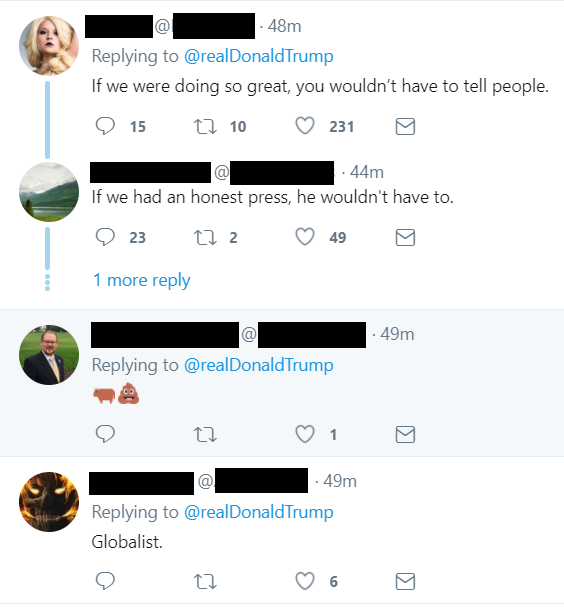
\includegraphics[width=.7\linewidth]{trump_tweets}
\end{figure}

Furthermore, discerning the meaning of tweets is doubly difficult in Arabic-language Twitter as existing computational linguistic models are usually limited to Western languages, and regional variants of Arabic, in addition to its non-standard Roman transliterations\footnote{Arabic-speaking social media users often write posts in an informal system known as Arabizi that matches Arabic letters with numbers when there is no Roman equivalent. However, users often made ad-hoc decisions in deciding how to transliterate Arabic vowels and verbal constructions, rendering it difficult to impossible to perform systematic grammatical analysis of the texts.}, make it hard to apply sentiment analysis without manually coding very large datasets. As a result, decisions over how to aggregate and measure tweets can have a strong influence on the results, and also make it difficult to compare across studies given the disparity in measurement strategies. In essence, the models and statistics that are computed on the aggregated data do not reflect the underlying uncertainty in the measurement of whichever latent social process the study is trying to capture. 

To respond to these concerns, we focus on a single type of Twitter-based behavior--retweets--and design a model that combines measurement with direct statistical analysis of ideological polarization. By so doing, our model only has to make two basic assumptions: 1) retweets are a signal of underlying ideological agreement and 2) our codings of elite Twitter users as Islamist or secularist are accurate. The first assumption has been shown to be valid through analyses of the political content of retweet networks \parencite{conover2011}. Every time a Twitter user clicks on the retweet icon by a tweet, they immediately broadcast it to their followers, signaling that the user believes this tweet is a message worth amplifying to their network.\footnote{Even though some users will say that their retweets do not signal agreement, in general it is rare to observe personal accounts doing so, as it is counter to the very idea of a personal account to amplify views that are reprehensible to one's own.} The second assumption of coding elite Twitter accounts, while still an assumption, is relatively transparent and easy to replicate, and we include the entire set of coding decisions in the appendix as a reference. All other analysis of ideology that we present in this paper flows from the model and incorporates the full uncertainty in accurately identifying the underlying social process of polarization relative to the irrelevant noise in the content of users' tweets. 

 To adequately model these phenomena, we borrow ideas from two distinct literatures in statistics: time-series econometrics, in particular vector auto-regression, and the item-response theory literature on estimating latent concepts. Item-response theory has been used in political science for estimating the latent positions of actors based on roll-call voting datasets \parencite{jackman2004}, and more recently, through social media and campaign finance contributions \parencite{bonica2014,barbera2015}. Item-response theory (IRT) has also been applied to difficult measurement problems, in particular the construction of democratization indices from a variety of coding sources \parencite{vdem2017,treier2008}. Item response models estimate latent traits for individual cases that can be divided into two distinct groups, such as raters and countries, lawmakers and bills, or in our sample, citizen and elite Twitter users. 

The main advantage of these models is that they are designed to provide latent estimates of fundamentally unobservable quantities, such as political ideology. For that reason, there is a strong connection between IRT and factor analysis \parencite{takane1986}, and similar concerns over the interpretation of the latent scores are justified. The latent dimension estimated by an IRT model will be the lowest-variance explanation of the observed data, but further prior knowledge and post-estimation validation is necessary to confirm that the results correspond with the concept of interest. We are confident in our application of this technique to the data because of our prior coding of users into similar ideological groups. For that reason, the resulting estimates will reflect these latent cleavages instead of arbitrary social behaviors or groupings. In other words, we anchor the model in our prior knowledge about elite users, and rely on the retweet patterns of ordinary users to see how these ideological networks are changing over time. As such, we define the latent scale in our model as inter-group distance rather than ideology per se because we are primarily examining polarization instead of changes in the content of the ideologies.

The existing application of time series modeling to IRT is limited despite the fact that political science has many time-varying variables with considerable measurement error. This paper builds on the approaches of \textcite{quinn2002} and \textcite{kropko2013} who use random-walk priors on latent-traits to incorporate change in ideal points over time. In time-series lingo, these latent traits become integrated variables that exhibit an infinite memory process: any shifts in the ideal points are remembered in the time series over time \parencite[Ch. 5]{timeseries2014}. While this type of autocorrelation is appropriate for long-term time series, our focus on short-run dynamics suggest we use a model that is based around stationary ideological groups, i.e., that groups receive random shocks causing heightened salience of ideological divides for a short period of time \parencite[Ch. 2]{timeseries2014}. In reality, ideological groups can exhibit both kinds of variation, with their evolution in the long-term taking any possible direction, including true ideological change such as conversion, while in the short-term the ideology of these groups is relatively fixed while the salience of ideological divides is variable \parencite{owen2010clash}. For this reason, we do not adopt the approach of \textcite{park2011}, who models ``preference regimes" as showing stasis over time with brief moments of change in a form of punctuated equilibrium, which is a model more suited for studying long-term changes in networks.

Finally, in addition to examining change over time, our research explores transnational ideological polarization. We want to know whether an increase in Islamist-secularist polarization in Egypt causes changes in Islamist-secularist polarization in Tunisia. For that reason, we need to look at multivariate time-series techniques, i.e., vector autogression (VAR). Vector autoregression involves the estimation of lags of different time series in the same equation \parencite{sims1980}, and has been used in political science to study time series that interact with each other for several decades \parencite{freeman1989}. Our main innovation in this paper is to fit a VAR and an IRT model simultaneously so that the VAR can fully incorporate the measurement error present in the Twitter data.

The primary purpose in employing a VAR as the inferential method is that it enables us to track the endogenous effects of the ideal points of Islamists and secularists on each other. To set up this model, we start with two time series that represent the latent ideal points of different religious groups: $y_{cgt}$ and $x_{-cgt}$. These series are observed at discrete time units $t$ and each belong to the same group $g \in \{Secularist, Islamist\}$ but different countries $c \in \{Tunisia, Egypt\}$. In a VAR framework, we can use the following equation to signify these series influencing each other through their prior period lags. The parameters $\beta_{cgIN}$ and $\beta_{cgOUT}$ control the relative influence of prior period lags:

\begin{align}\label{var}
	y_{cgt} &= \gamma_{cg} + \beta_{cgIN}y_{cgt-1} + \beta_{cgOUT}x_{-cgt-1} + \beta_{gcx}X  + \epsilon_{cgt}\\
	x_{-cgt} &= \gamma_{-cg} + \beta_{-cgIN}x_{-cgt-1} + \beta_{-cgOUT}y_{cgt-1} + \beta_{g-cx}X + \epsilon_{-cgt}
\end{align}

To make the model stochastic, we include $\epsilon_{cgt}$ and $\epsilon_{-cgt}$ as white noise (stationary) errors so long as $\beta_{cgIN}$ and $\beta_{cgOUT}$ meet the VAR stability conditions \parencite[386-387]{zivot2006}.\footnote{Loosely speaking, a VAR is stationary if the eigenvalues of the coefficients of the lags in the VAR have a modulus less than one. In essence, if these coefficients are too large in absolute terms relative to each other, the VAR will move away from its equilibrium level in either a random or explosive direction.} So long as these parameters meet the stability conditions, the latent ideal points will over time return to their long-run equilibrium value $\gamma_{cg}$ (i.e., the intercept). Substantively, these parameters provide estimates of how quickly a time series will return to its long-term mean given an exogenous shock ($\beta_{cgIN}$) and the strength of influence of the other time series ($\beta_{cgOUT}$).\footnote{We only include one lag of each series in our VAR equation because the time series are themselves latent variables, and as such the normal lag selection procedures for VARs do not apply. We would prefer as well to keep the model as parsimonious as possible.}

We also include an additional parameter in each series, $\beta_{gcx}$. This parameter does not vary over time and rather represents the effect of the exogenous event $X$, which equals 1 after the coup against President Morsi in Egypt and 0 before the coup. As such, we can use $\beta_{gcx}$ as a direct measure of the long-term polarizing effect of the coup on each of the series. A null hypothesis of no effect of the coup would be the case in which $\beta_{gcx}=0$.

Given that we have two groups and two countries, we have two sets each of ideal points series $y_{cgt}$ and $x_{-cgt}$ for a four time-series system (Tunisian secularists and Islamists and Egyptian secularists and Islamists). While we could pair each series with every other series, we instead chose to only pair each ideological group with their co-religionists in the other country. We impose this restriction because we aim to identify the effect of transnational polarization, and also because the within-country groups are separately related through the IRT model that we explicate in the appendix.

Given this framework, we are able to track endogenous changes in the latent ideal point time series via the coefficients $\beta_{cgIN}$ and $\beta_{cgOUT}$ that provide evidence of how reactive groups are to their own prior ideological position and to the position of other groups. A small value of $\beta_{cgOUT}$ will imply that a religious group is relatively insensitive to the actions of their foreign co-religionists, and a larger value that the religious group is very sensitive to what happens in other countries. On the other hand, a small value of $\beta_{cgIN}$ implies that a religious group is relatively insensitive to its own prior position in the latent space. As such, a low value of this parameter also signifies the stability of the series. Supposing that the religious group experienced some kind of shock that heightened the salience of religious divides, a lower $\beta_{cgIN}$ will imply that the group return quickly to the long-term mean of the series (the intercept $\gamma_{cg}$). By contrast, a higher value of $\beta_{cgIN}$ implies that the religious group is unstable and is unlikely to return quickly to a long-term mean. If $\beta_{cgIN} = 1$ the series is very unstable and may not ever return to a long-term mean.

However, we need to obtain the ideal point series themselves ($y_t$ and $x_t$) in order to calculate all of these effects. As we mentioned earlier, we cannot directly measure ideological agreement on Twitter. We could try to create relevant time series by aggregating our Twitter data around the content of tweets using particular key words or hashtags, such as the Arabic phrases for sectarian terms. However, as we mentioned earlier, that would make our analysis heavily dependent on the particular set of keywords we chose to employ. For that reason, to estimate the underlying latent estimates using a more principled approach, we turn to item-response theory (IRT).

We provide a full explication of how we combine IRT and the VAR in Appendix B as well as explain how we can estimate this model using Bayesian inference. In essence, we use IRT to create the time series which are then fed into the VAR. IRT converts the raw Twitter data into four latent variables that represent the group-level ideal points of each of the religious-country groups. Because our IRT model uses the ideal point formulation \parencite{jackman2004}, the resulting latent variables can be interpreted as the relative position of the groups in a latent social space. Distance in this space then represents the closeness of these groups to each other in terms of social salience. For example, as group polarization increases within countries, we would expect the ideal points of two groups within countries to move farther apart in the latent space. Empirically that polarization would be expressed as more strongly polarized retweet patterns, but the IRT model is able to reduce that high-dimensional and rather noisy data down to a single estimate with a credible interval to indicate our uncertainty in its true location.


 To test the model, we simulated data by generating ideal points corresponding to the VAR equation above. The simulated ``true" latent time series, each of which is paired with another time series representing an ideological group in different country, is shown in Figure \ref{sim_data}. As can be seen, the two sets of time series each follow a pattern over time that is roughly stationary.
 \begin{figure}[!h]
 	\caption{Simulated Data for the Vector Auto-regressive Component of IRT-VAR}\label{sim_data}
 	\centering
	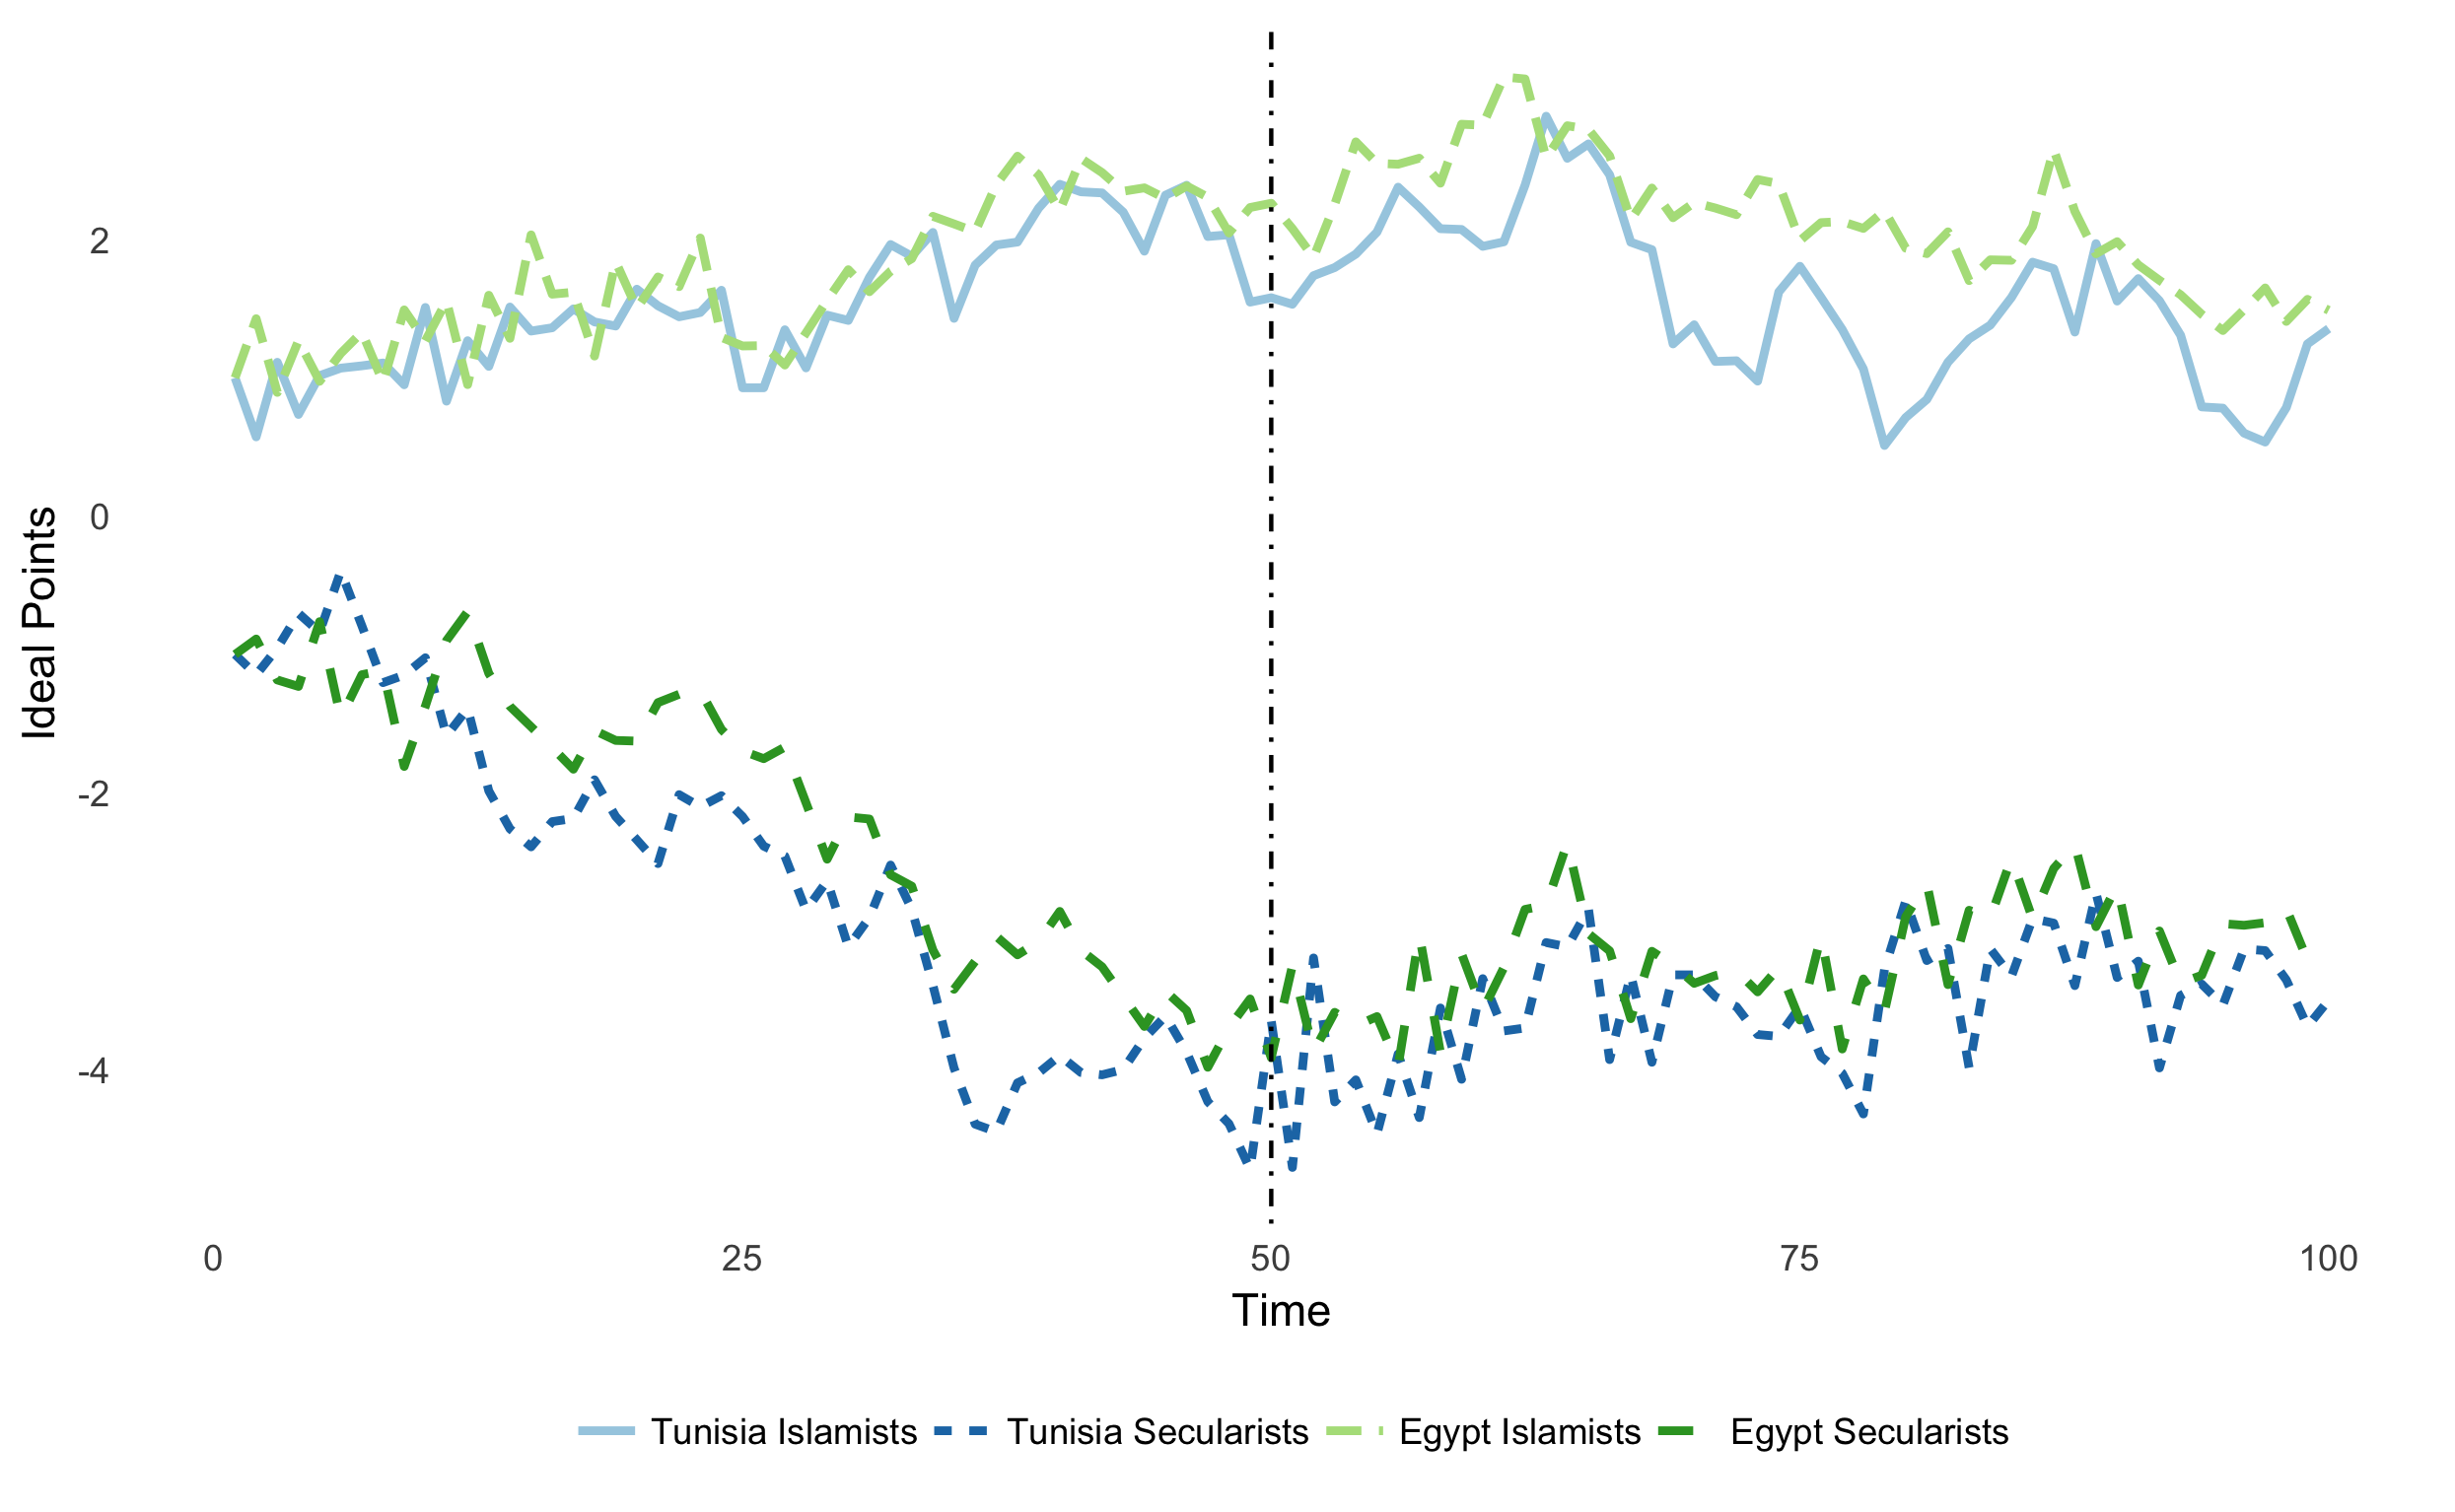
\includegraphics[width=.9\linewidth]{ecm_example.png}
 \end{figure}

The vertical line in Figure \ref{sim_data} shows the time period where an exogenous event $X$ occurs and $\beta_{gcx}$ has a non-zero value, which will shift the long-run equilibrium of each time series depending on the value of $\beta_{gcx}$. In addition to the summary estimate of $\beta_{gcx}$, we can also use the values of $\beta_{cgIN}$ and $\beta_{cgOUT}$ to calculate impulse-response functions (IRFs) for a shock to the elite group's ideal points coming from the group's own time series, or the indirect effect coming from a shock to a different group's time series. We can express this mathematically as the derivative of an exogenous shock $\epsilon_{cgt}$ with respect to the value of the ideal point $\alpha_{cgt}$ at time points after the shock from $t+n, n\in \{1,2,...10\}$:
\begin{equation}
\frac{\partial \alpha_{cg(t+n)}}{\partial \epsilon_{cgt}}
\end{equation}

This IRF essentially measures the decaying (if the time series is stable) average effect of a shock to the latent ideal points over time, and provides a straightforward measure of influence in the time series. We can use this same framework to calculate other IRFs of interest, including the influence of an exogenous shock to co-religionists in another country,

\begin{equation}
\frac{\partial \alpha_{cg(t+n)}}{\partial \epsilon_{-cgt}}
\end{equation}

the influence of the exogenous event $X$,

\begin{equation}
\frac{\partial \alpha_{cg(t+n)}}{\partial \beta_{gcx}}
\end{equation}

the influence of the exogenous event $X$ working through its polarizing effect on ideological allies in another country (i.e., indirect effects of the exogenous event):

\begin{equation}
\frac{\partial \alpha_{cg(t+n)}}{\partial \beta_{g-cx}}
\end{equation}

and the combined influence of the exogenous event $X$ on the within-country group $\alpha_{cgt}$ and the other country group $\alpha_{-cgt}$ (the combined effect):

\begin{equation}
\frac{\partial \alpha_{cg(t+n)}}{\partial \beta_{gcx}\partial \beta_{g-cx}}
\end{equation}

To summarize the model, then, we can match these estimates to our hypotheses to provide very specific null hypothesis tests of our arguments that, as we have noted, incorporate our measurement uncertainty in using Twitter data into the tests. We show how this model relates to our hypothess in Table \ref{Htests}.
\begin{table}[h!]
	\centering
	\caption{Hypotheses and Associated Tests from our Model}\label{Htests}
	\scriptsize
	\begin{tabular}{lp{7cm}l}
		Hypothesis & Definition & Expected Outcome\\
		H1 & As the latent ideological position of Islamists or secularists changes, the latent ideological position in the like-minded group in the other state will also change. & $\frac{\partial \alpha_{cg(t+n)}}{\partial \epsilon_{-cgt}}\neq0$ for all $c \in C$ and $g \in G$\\[1em]
		H2 & After the coup against Mohammed Morsi, the difference in latent ideological positions between Islamists and secularists will diverge in direct reaction to the coup (direct effect). & $\frac{\partial \alpha_{cg(t+n)}}{\partial \beta_{gcx}}\neq0$ for all $c \in C$ and $g \in G$\\[1em]
		H3 & After the coup against Mohammed Morsi, the difference in latent ideological positions between Islamists and secularists will diverge from each group's reaction to their ideological allies' shift in latent ideological position (indirect effect). & $\frac{\partial \alpha_{cg(t+n)}}{\partial \beta_{g-cx}}\neq0$ for all $c \in C$ and $g \in G$\\[1em]
		H4 & After the coup against Mohammed Morsi, the difference in latent ideological positions between Islamists and secularists from the direct reaction to the coup and each group's reaction to their ideological allies' shift will be greater than the direct reaction to the coup alone (combined effect). & $\frac{\partial \alpha_{cg(t+n)}}{\partial \beta_{gcx}\partial \beta_{g-cx}}\neq0$ for all $c \in C$ and $g \in G$
	\end{tabular}
\end{table}

As this model has not been previously estimated in the literature, we also perform a simulation study in which we sample from the data-generating process and test to make sure we can recover both the parameter values and the correct values of the IRFs. The results of this study in Appendix B show that our use of Bayesian inference is able to capture the latent process even with non-ignorable missingness in the outcome, which occurs in Twitter often as Twitter users tend to self-select which tweets they are likely to see on a given day in terms of their ideological proximity by following a specific set of elites.

\section*{Model Results}

Estimating this model using full Bayesian inference would be computationally prohibitive given the size of the data. To address this big data issue, we employ variational Bayesian inference in which we estimate an approximation to the true posterior by minimizing the Kullback-Leibler divergence between the true posterior and a Normal mixture approximation using the Stan estimation engine \parencite{NIPS2015_5758}. Any additional error created by the use of an approximation is a minimal concern given the size of the data and the asymptotic properties of minimizing KL divergence \parencite{grimmer2011,NIPS2015_5758}. Our variational estimation produced latent parameters for all 18,123 of the citizens in the model, but we instead focus on the four group parameters that varied over time, $\alpha_{cgt}$, one for each country-ideological pairing: Tunisian secularists, Egyptian secularists, Tunisian Islamists, and Tunisian secularists, as they are our primary focus for inference.

We first present a plot showing the estimated ideal points for the four ideological groups along with a vertical line showing when the military coup against Mohammed Morsi occurred. The confidence intervals on the chart reflects the 10\%-90\% density region of the approximated posterior, hereafter referred to as the high-posterior density (HPD) interval. From this chart we can make useful descriptive inferences. First, it is clear that in terms of latent inter-group distance, the Islamists are much closer to each other than are the secularists in either country. Substantively, this finding means that Islamist Twitter users share much more in terms of the sectarian nature of their retweet patterns relative to secularists. Again, these latent estimates do not necessarily measure the content of beliefs, but rather the relative salience of these ideological divides and the way that these divides manifest themselves on Twitter. Secularists in both countries are farther apart in our latent space because citizens' tweet patterns would not indicate much ideological salience across the groups' networks. 
 \begin{figure}[!h]
 	\centering
	\caption{Estimated Ideal Point Locations for Transnational Ideological Groups}\label{arab_id_facet}
	\centering
	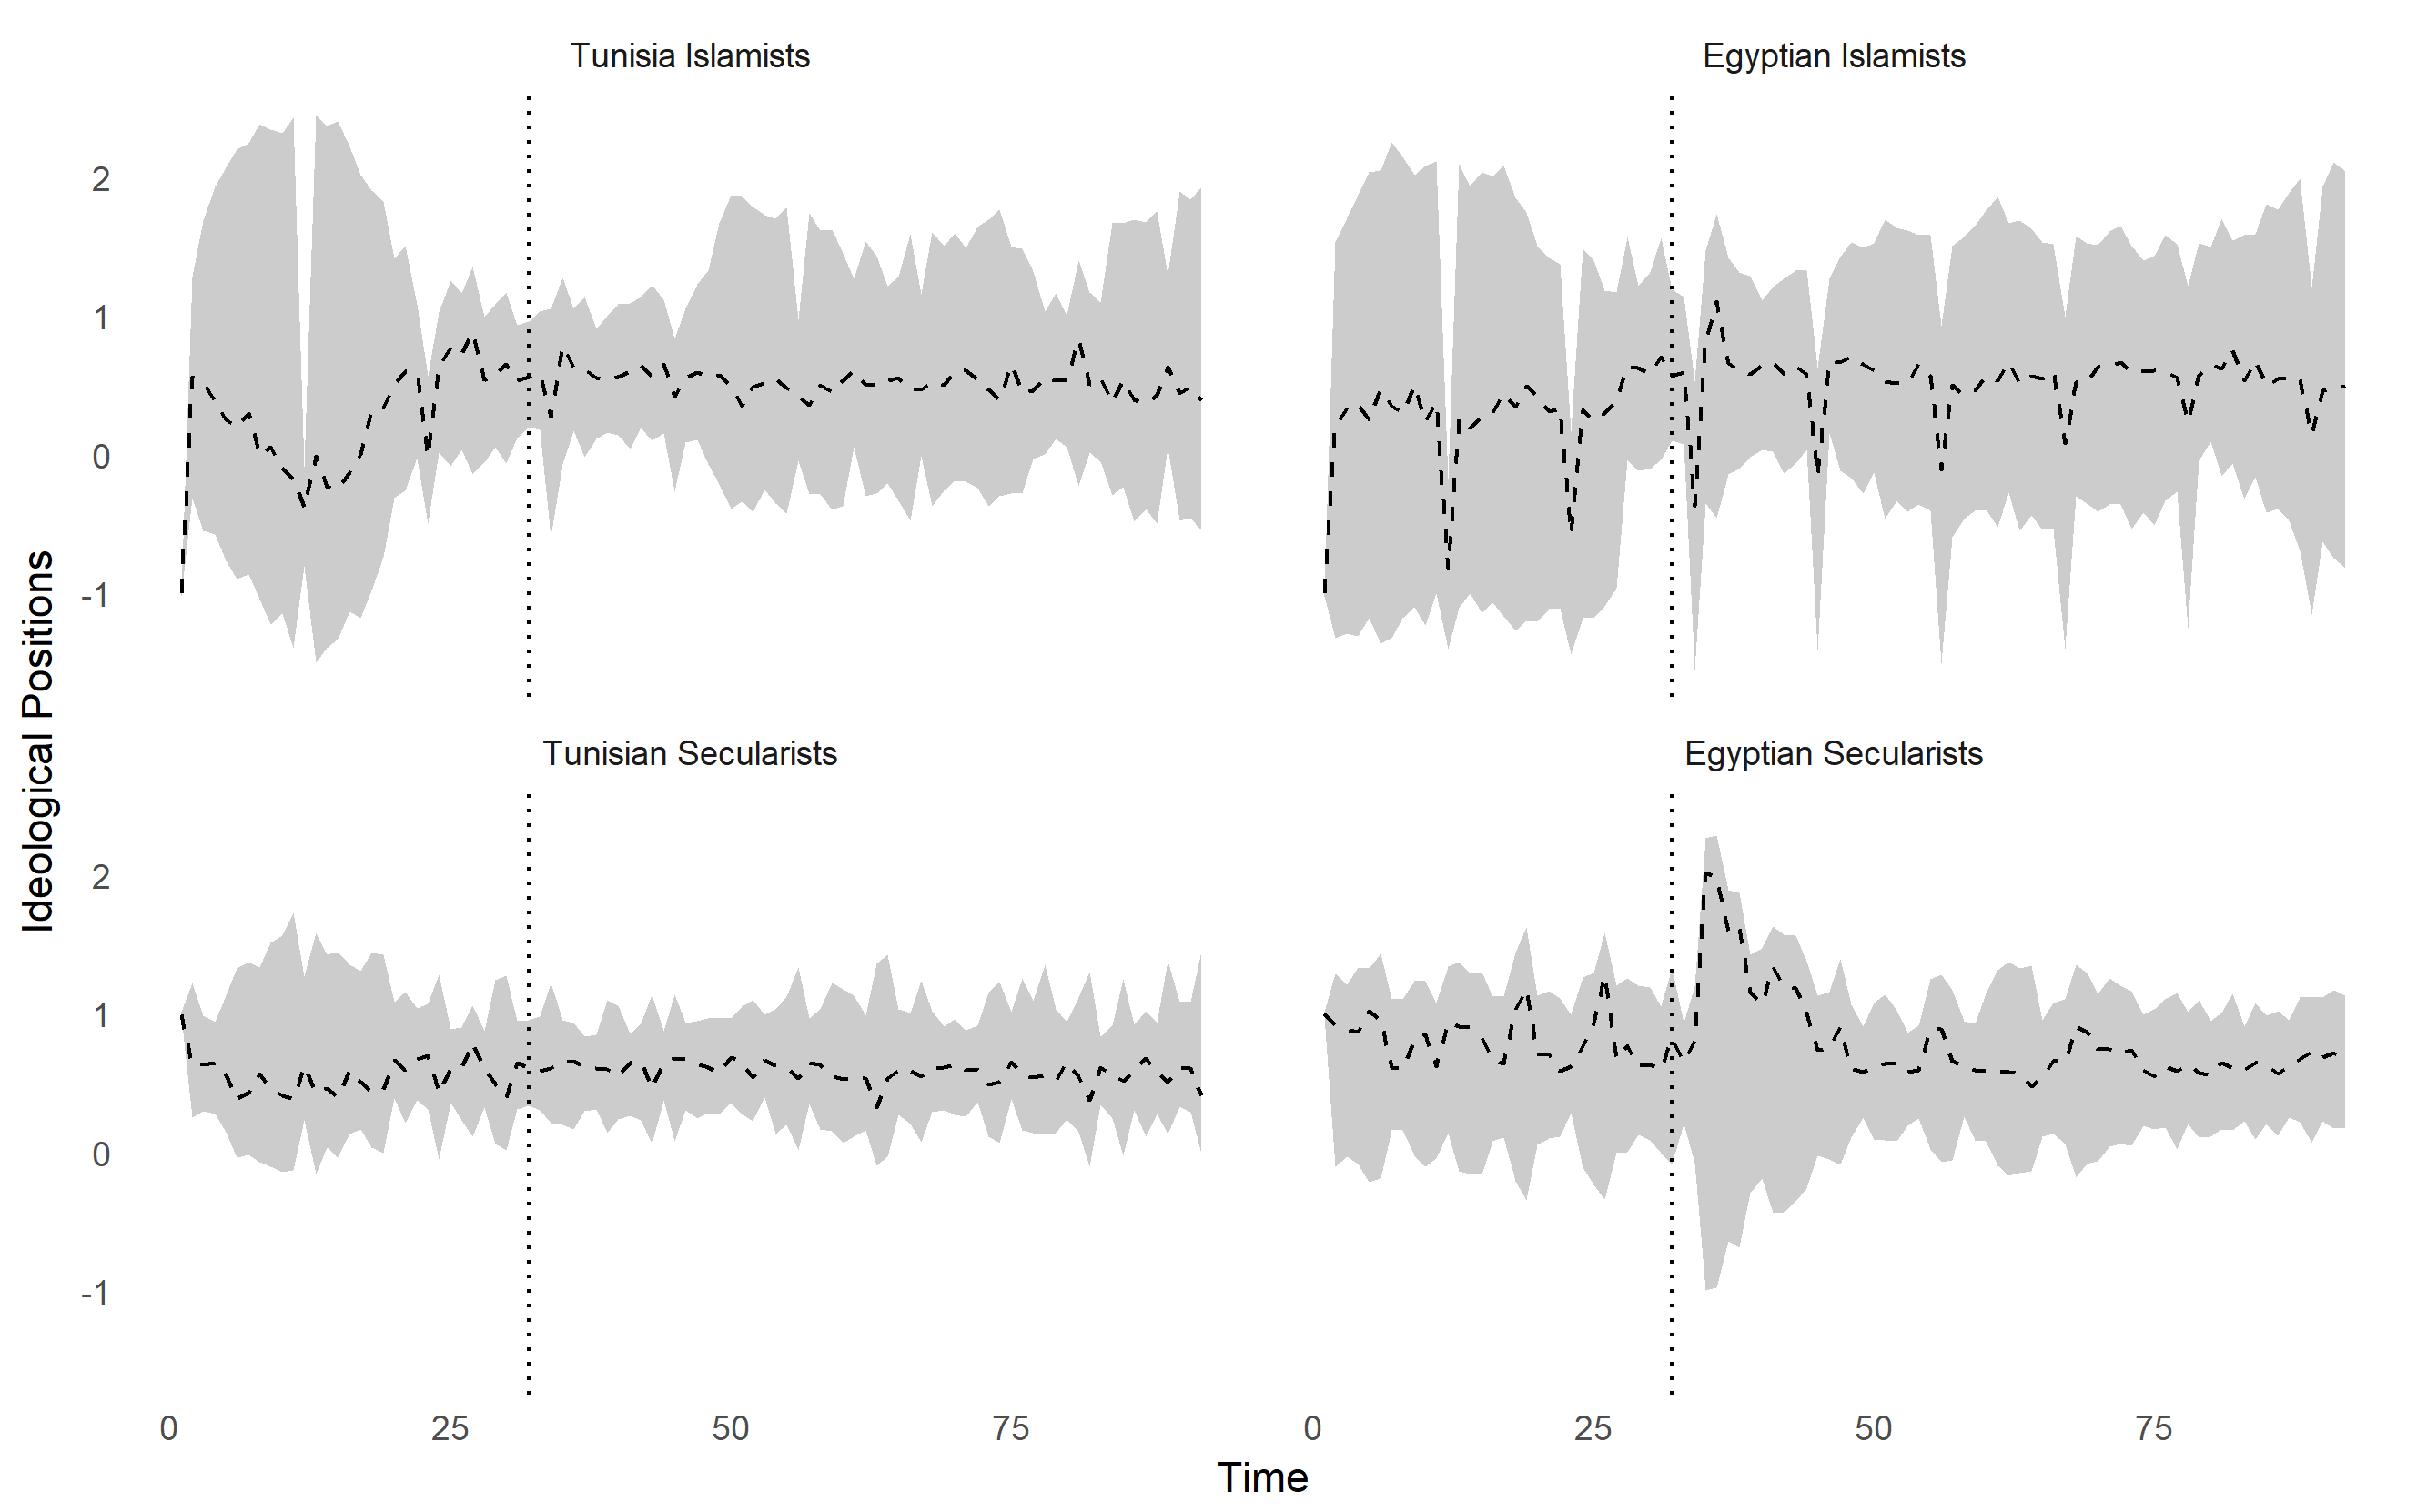
\includegraphics[width=.9\linewidth]{arab_ideology}
\end{figure}

In addition, Figure \ref{arab_id_facet} reveals that other events seemed to have a greater effect in terms of shifting ideal points than the Morsi coup that we focus on. The single largest movement appears in the ideal points of Tunisian secularists, and can be traced to the promulgation of a draft constitution that occurred on April 25, 2013. This draft modified wording in the constitution that diluted language about human rights in favor of Tunisia's ``cultural specificities" that was widely interpreted as an attempt by the ruling Islamist party in Tunisia to provide guarantees that the relatively secular human rights language could not be used against Islamic norms \parencite{hrw2013}. With the caveat of hindsight, it makes sense that this event would prove to be so directly polarizing as it involved a change to the basic law of Tunisia's governance that corresponded closely to latent social cleavages.

Other events are also noticeable from the plot, including the assassination of Mohammed Brahmi, a secularist politician, allegedly by Islamist radicals in July of 2013. We also see a noticeable spike in the Egyptian Islamists ideal points during the time of the Rabaa massacre, when the Egyptian military violently suppressed a sit-in by Muslim Brotherhood members opposing the coup against Muhammed Morsi. Given that these spikes in ideal points conform closely to events that we can identify as polarizing, but which we did not necessarily  identify in advance (especially Tunisia's draft constitution), the estimated latent dimension appears to correspond closely to our label of ``inter-group distance" as a measure of ideological polarization.

 To see the relationships better, we show these time-varying ideal points without HPD intervals and overlapping country/ideological groups in Figures \ref{arab_id_facet} and \ref{country_facet}. While it can be difficult to spot patterns in time series with the naked eye, it is very clear that Islamists track with each other much more than secularists do in general, and that Tunisians tended to mirror each other more closely than Egyptians. Furthermore, while the opposing groups within countries are on average the same distance apart, Egyptian secularists and Islamists are farther apart on average than their Tunisian counterparts. To discern more clearly whether inter-group distance is greater in one country, Figure \ref{diffindiff} shows the difference of the within-country inter-group differences in ideal point locations between Egypt and Tunisia. During the Tunisian constitutional crisis, within-country polarization (i.e., difference in ideal point locations) in Tunisia was significantly greater than Egypt's, but after Morsi's coup, Egypt's within-country polarization remained consistently higher than Tunisia's until the end of 2013.
 \begin{figure}[!h]
 	\centering
	\caption{Estimated Ideal Point Locations by Religion}\label{religion_facet}
	\centering
	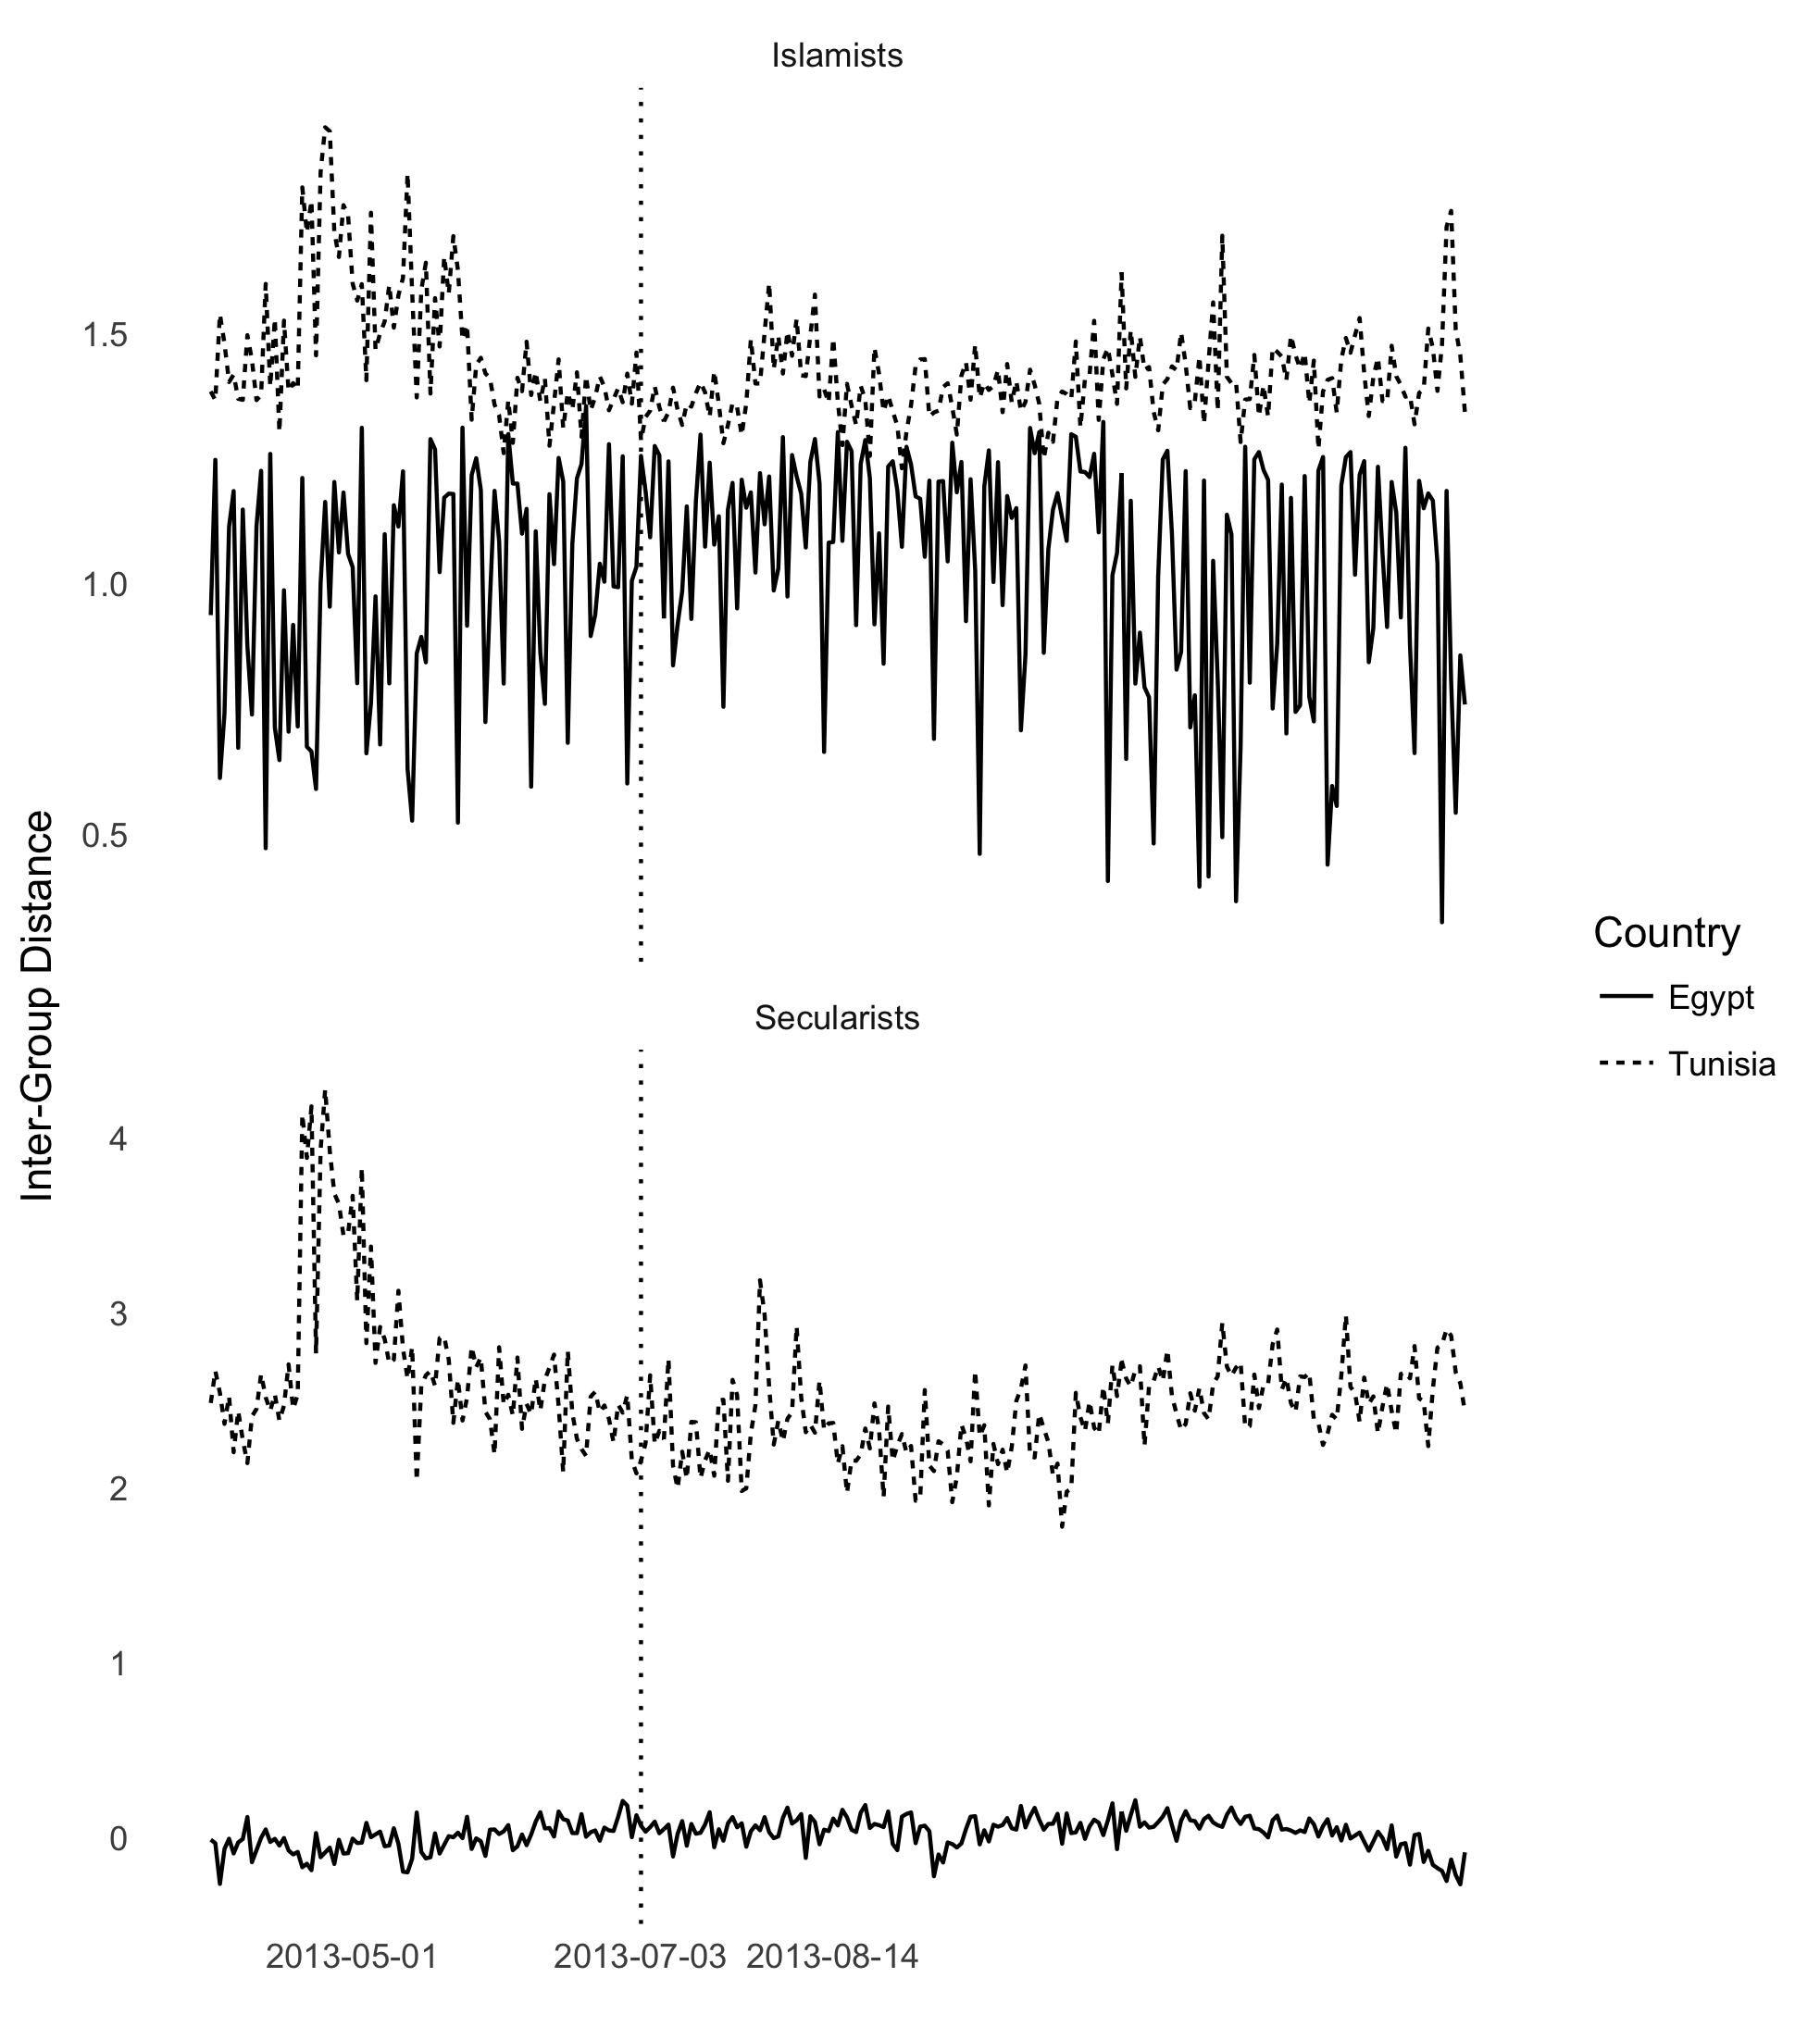
\includegraphics[width=.9\linewidth]{religion_coint}
\end{figure}
 \begin{figure}[!h]
 	\centering
	\caption{Estimated Ideal Point Locations by Country}\label{country_facet}
	\centering
	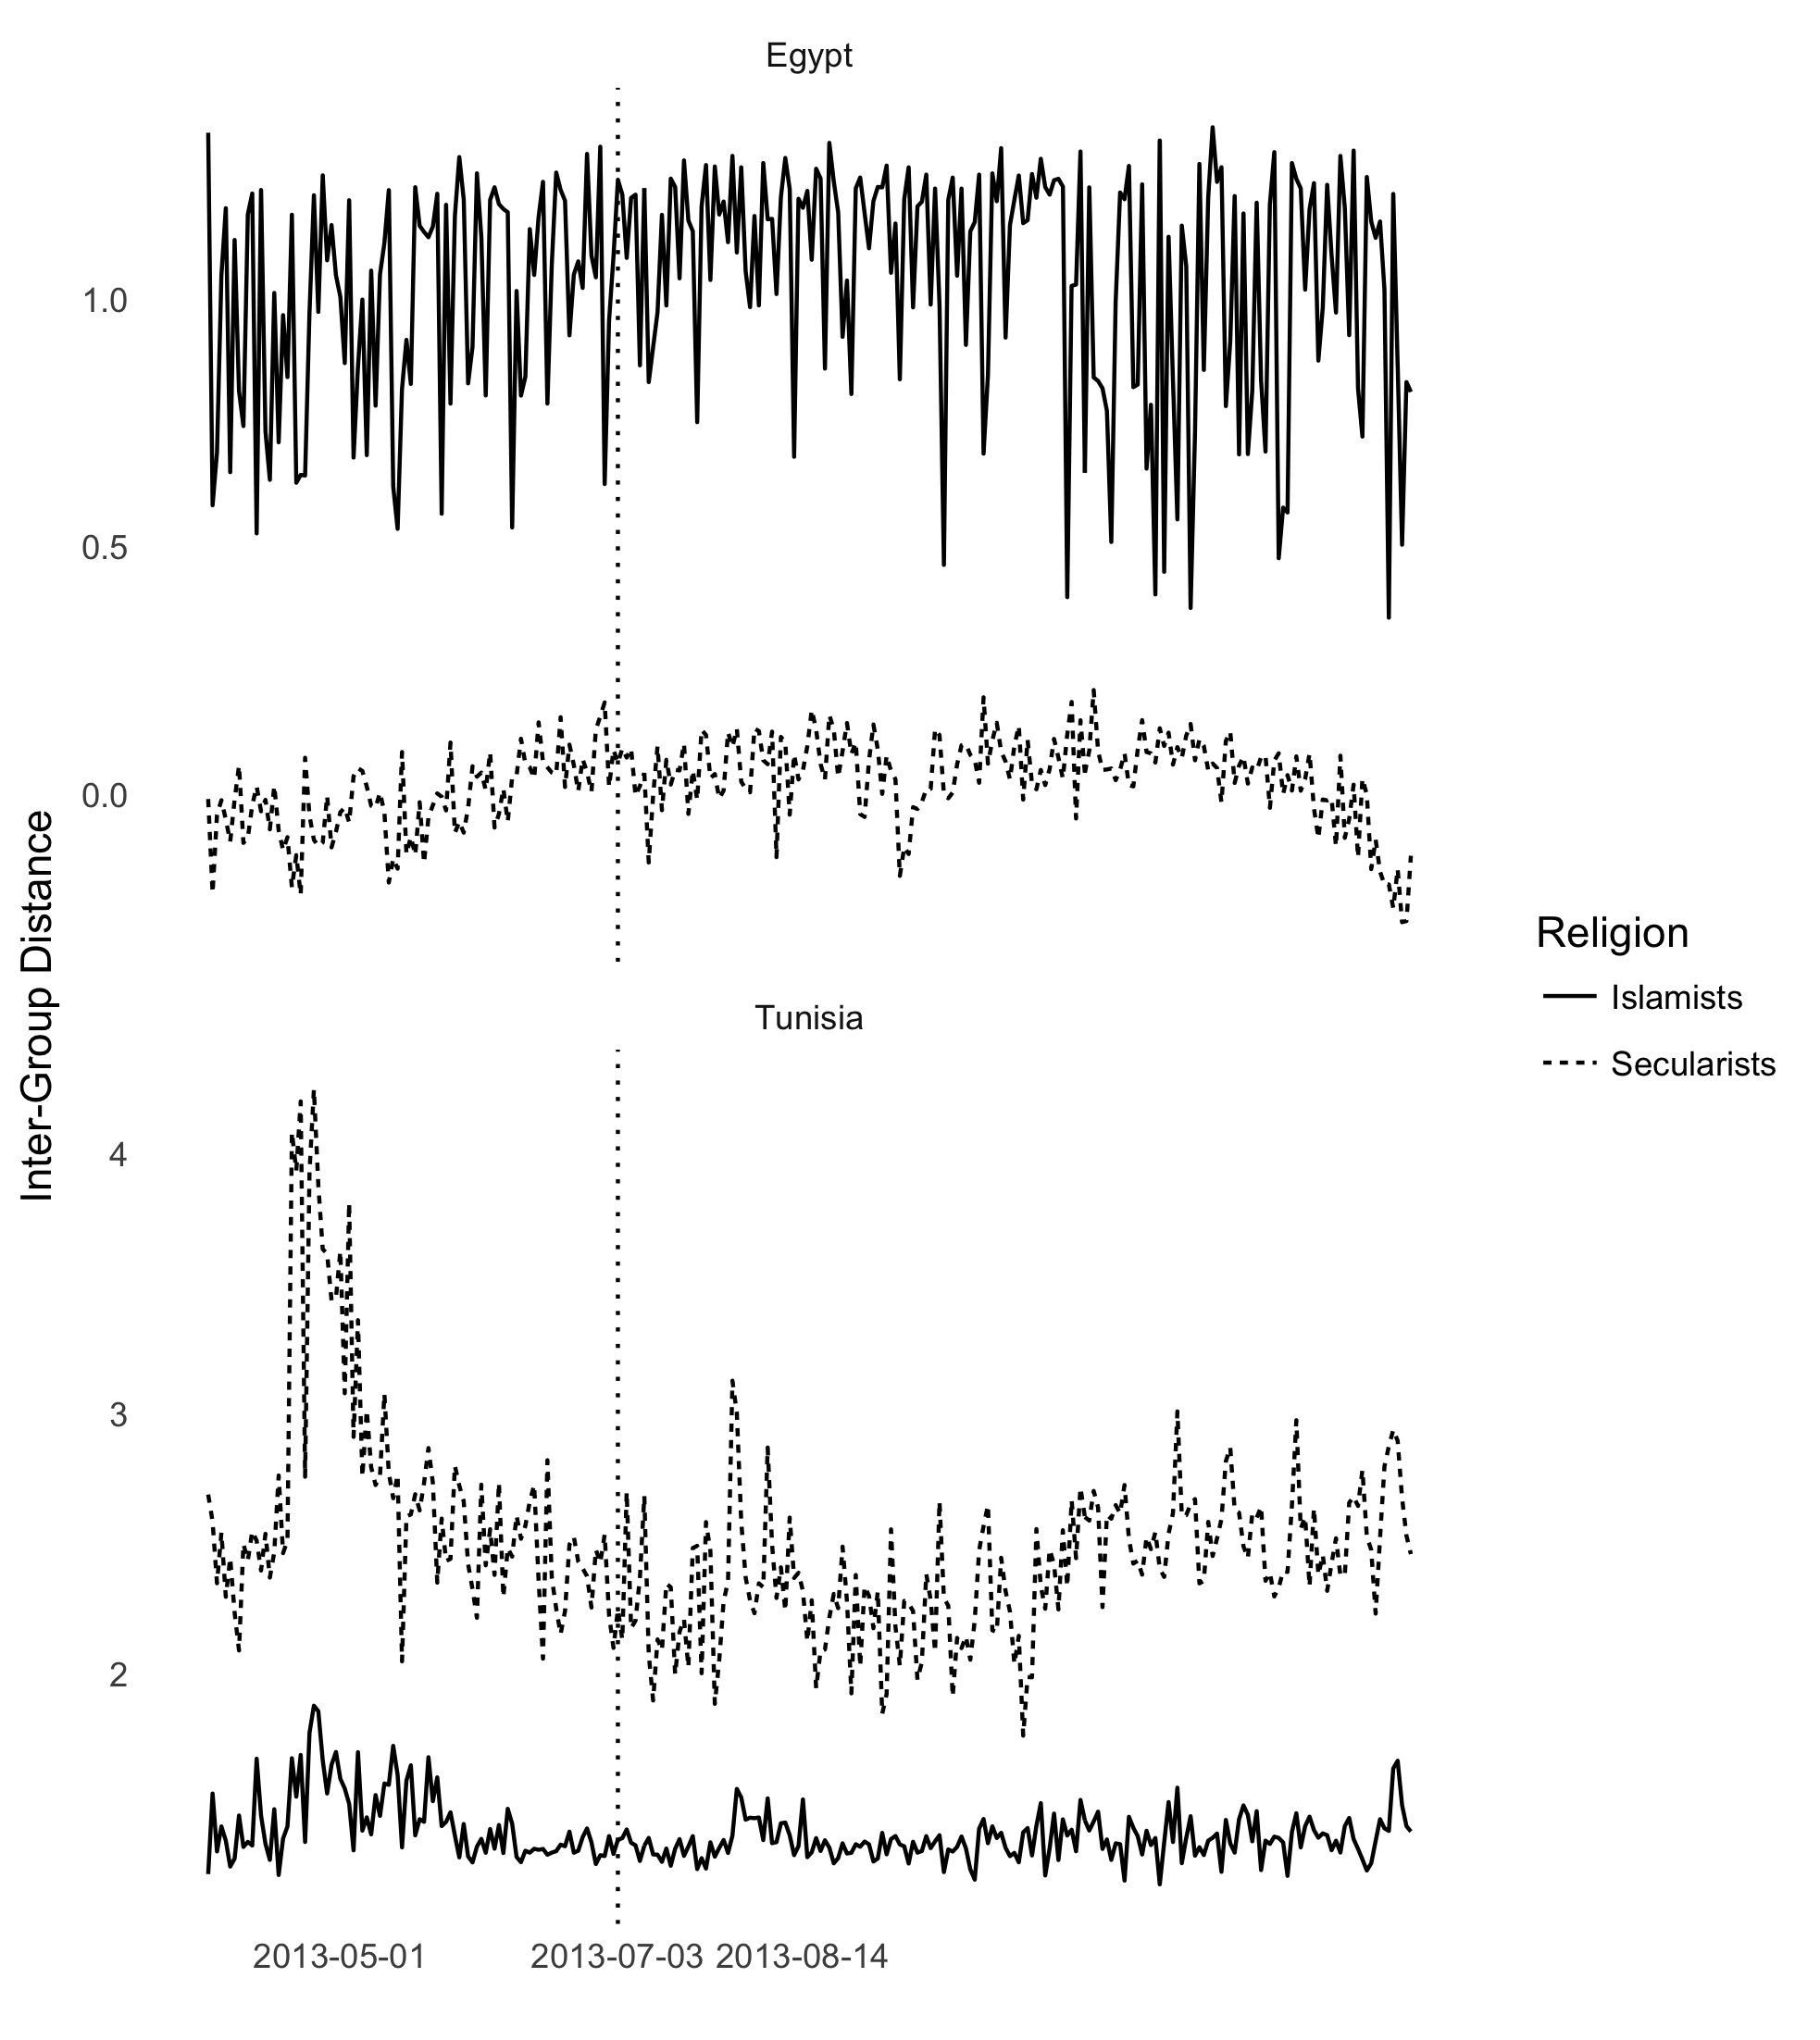
\includegraphics[width=.9\linewidth]{country_coint}
\end{figure}
 \begin{figure}[!h]
	\centering
	\caption{Difference-in-Difference Between Within-Country Ideological Groups' Ideal Points}\label{diffindiff}
	\centering
	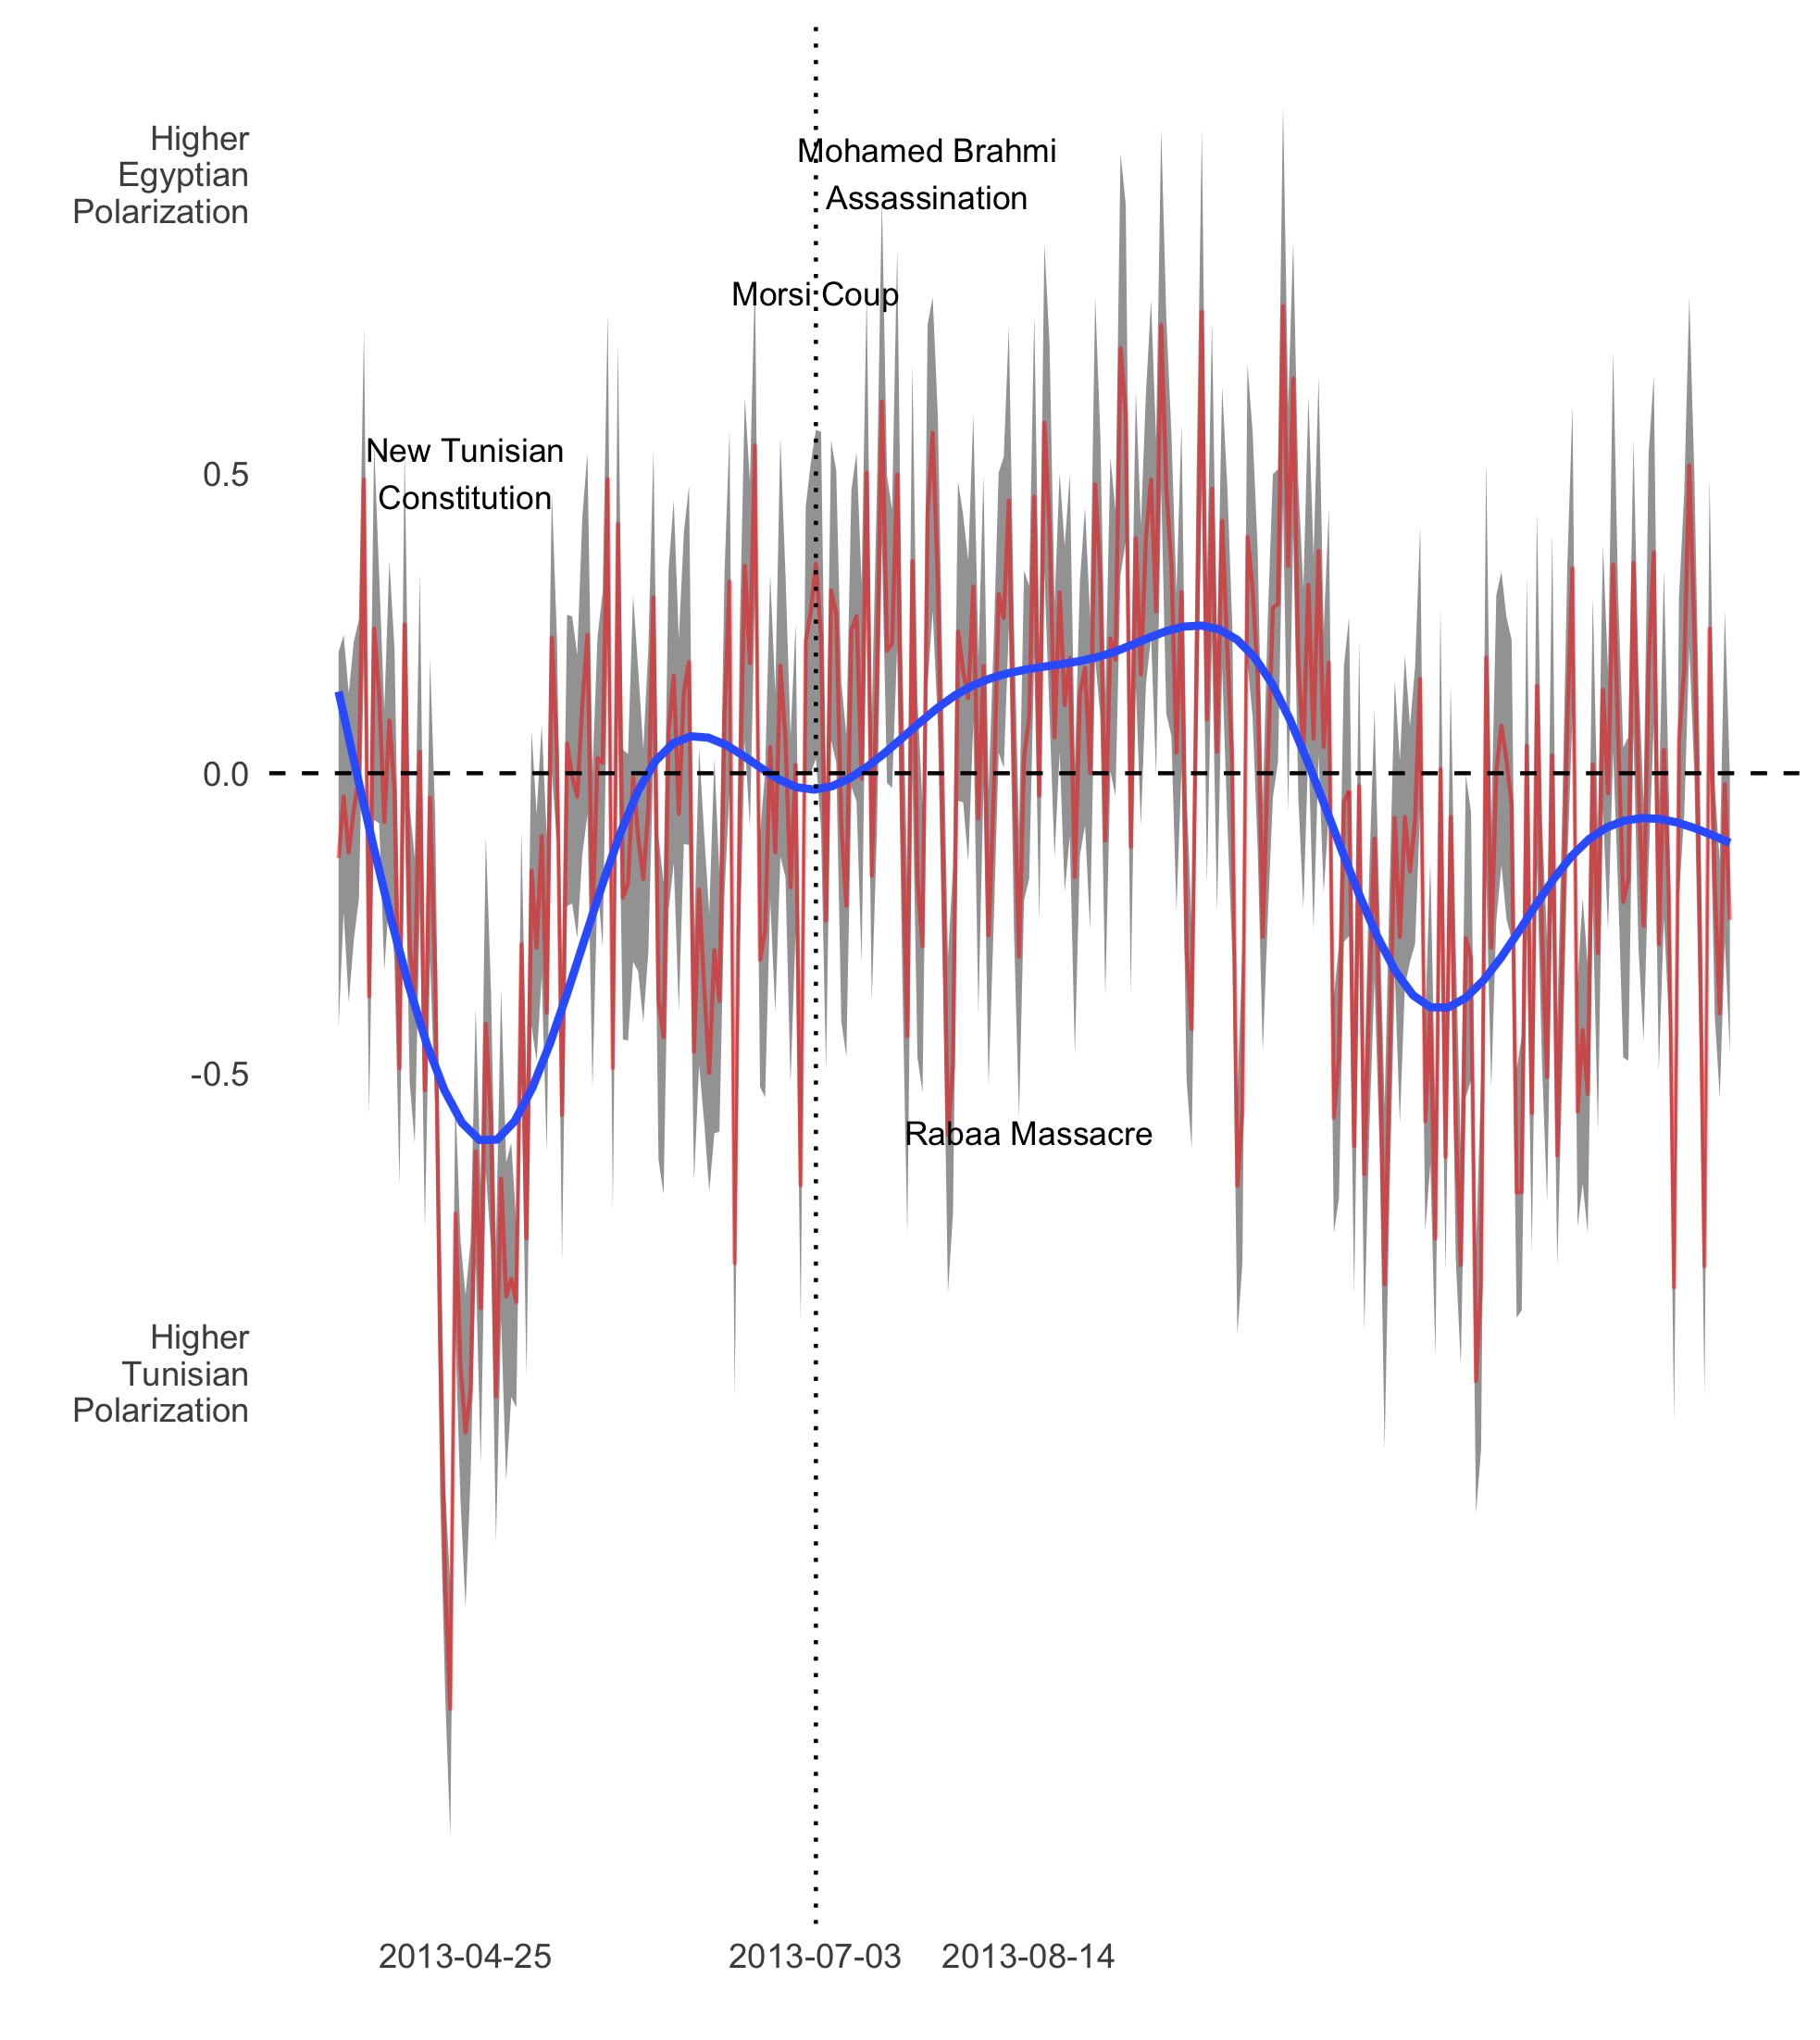
\includegraphics[width=.9\linewidth]{diff_ideal}
\end{figure}



Next we present the parameters from the VAR component of the model in Figure \ref{varparam}. This plot of the posterior densities of the adjustment parameters $\beta_{cgIN}$ and $\beta_{cgOUT}$ provides a precise definition of how ideological groups react to each other and to their own prior history. First, $\beta_{cgIN}$ captures how strongly the ideological group is influenced by its recent past as opposed to its long-run value. In other words, a higher value of  $\beta_{cgIN}$ implies that the ideological group is relatively unstable and likely to drift in an uncertain direction, whereas a lower value of $\beta_{cgIN}$ means that the ideological group remains fixed around its long-term inter-group distance and, although it will respond to shocks, its position in the system is relatively fixed. What is of interest with these parameters is that the $\beta_{cgIN}$ parameters are much higher for secularists than for Islamists. Tunisian secularists have a value that is greater than 0.5, which reflects the random-walk nature of the time series seen in Figure \ref{arab_id_facet}. What these parameter values imply is that secularists tend to less fixed in their relative position within the system, and a shock to their ideal point values will last much longer. By comparison, Islamists are fixed around their long-term mean; while they will certainly respond to shocks there is little long-term movement away from their central location in this latent space. Substantively, one could say that the Islamists have a much more coherently formed movement than the secularists.
 \begin{figure}[!h]
	\centering
	\caption{Estimated Adjustment Parameters $\beta_{cgIN}$ and $\beta_{cgOUT}$ from IRT-VAR Model}\label{varparam}
	\centering
	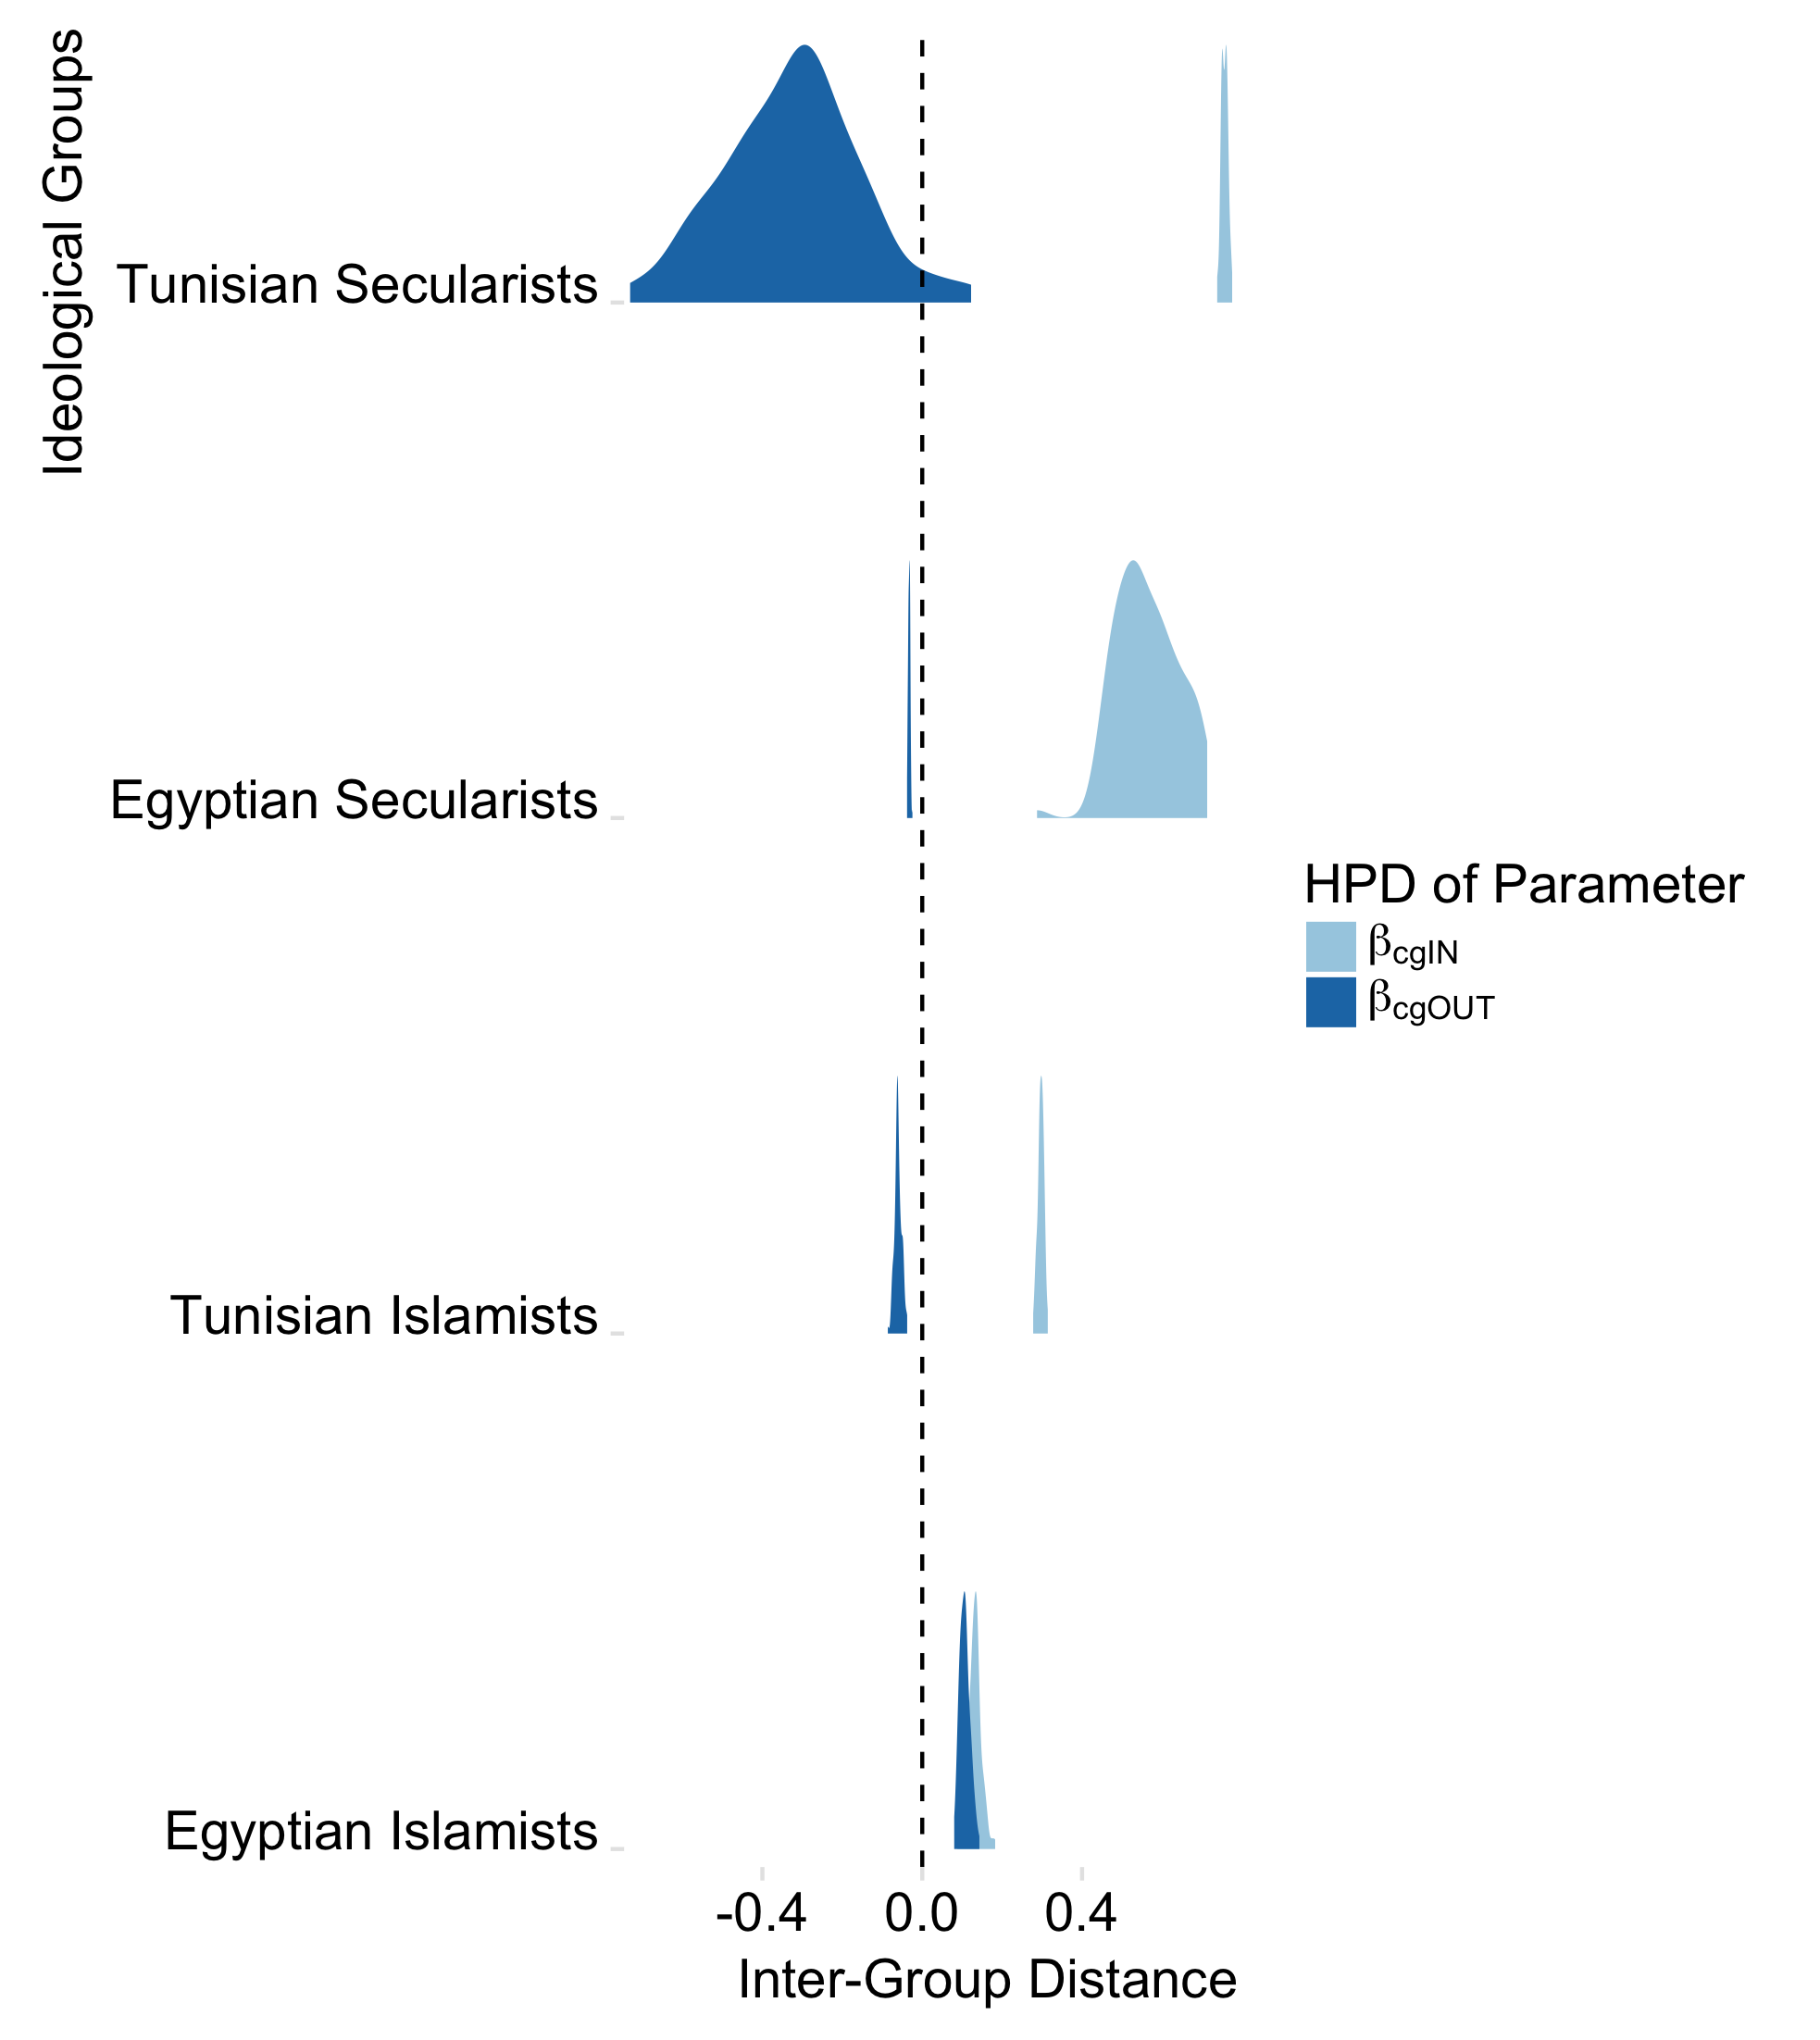
\includegraphics[width=.9\linewidth]{adj_par}
\end{figure}
 \begin{figure}[!h]
	\centering
	\caption{Estimated Coup Effect $\beta_{cgx}$ from IRT-VAR Model}\label{betax}
	\centering
	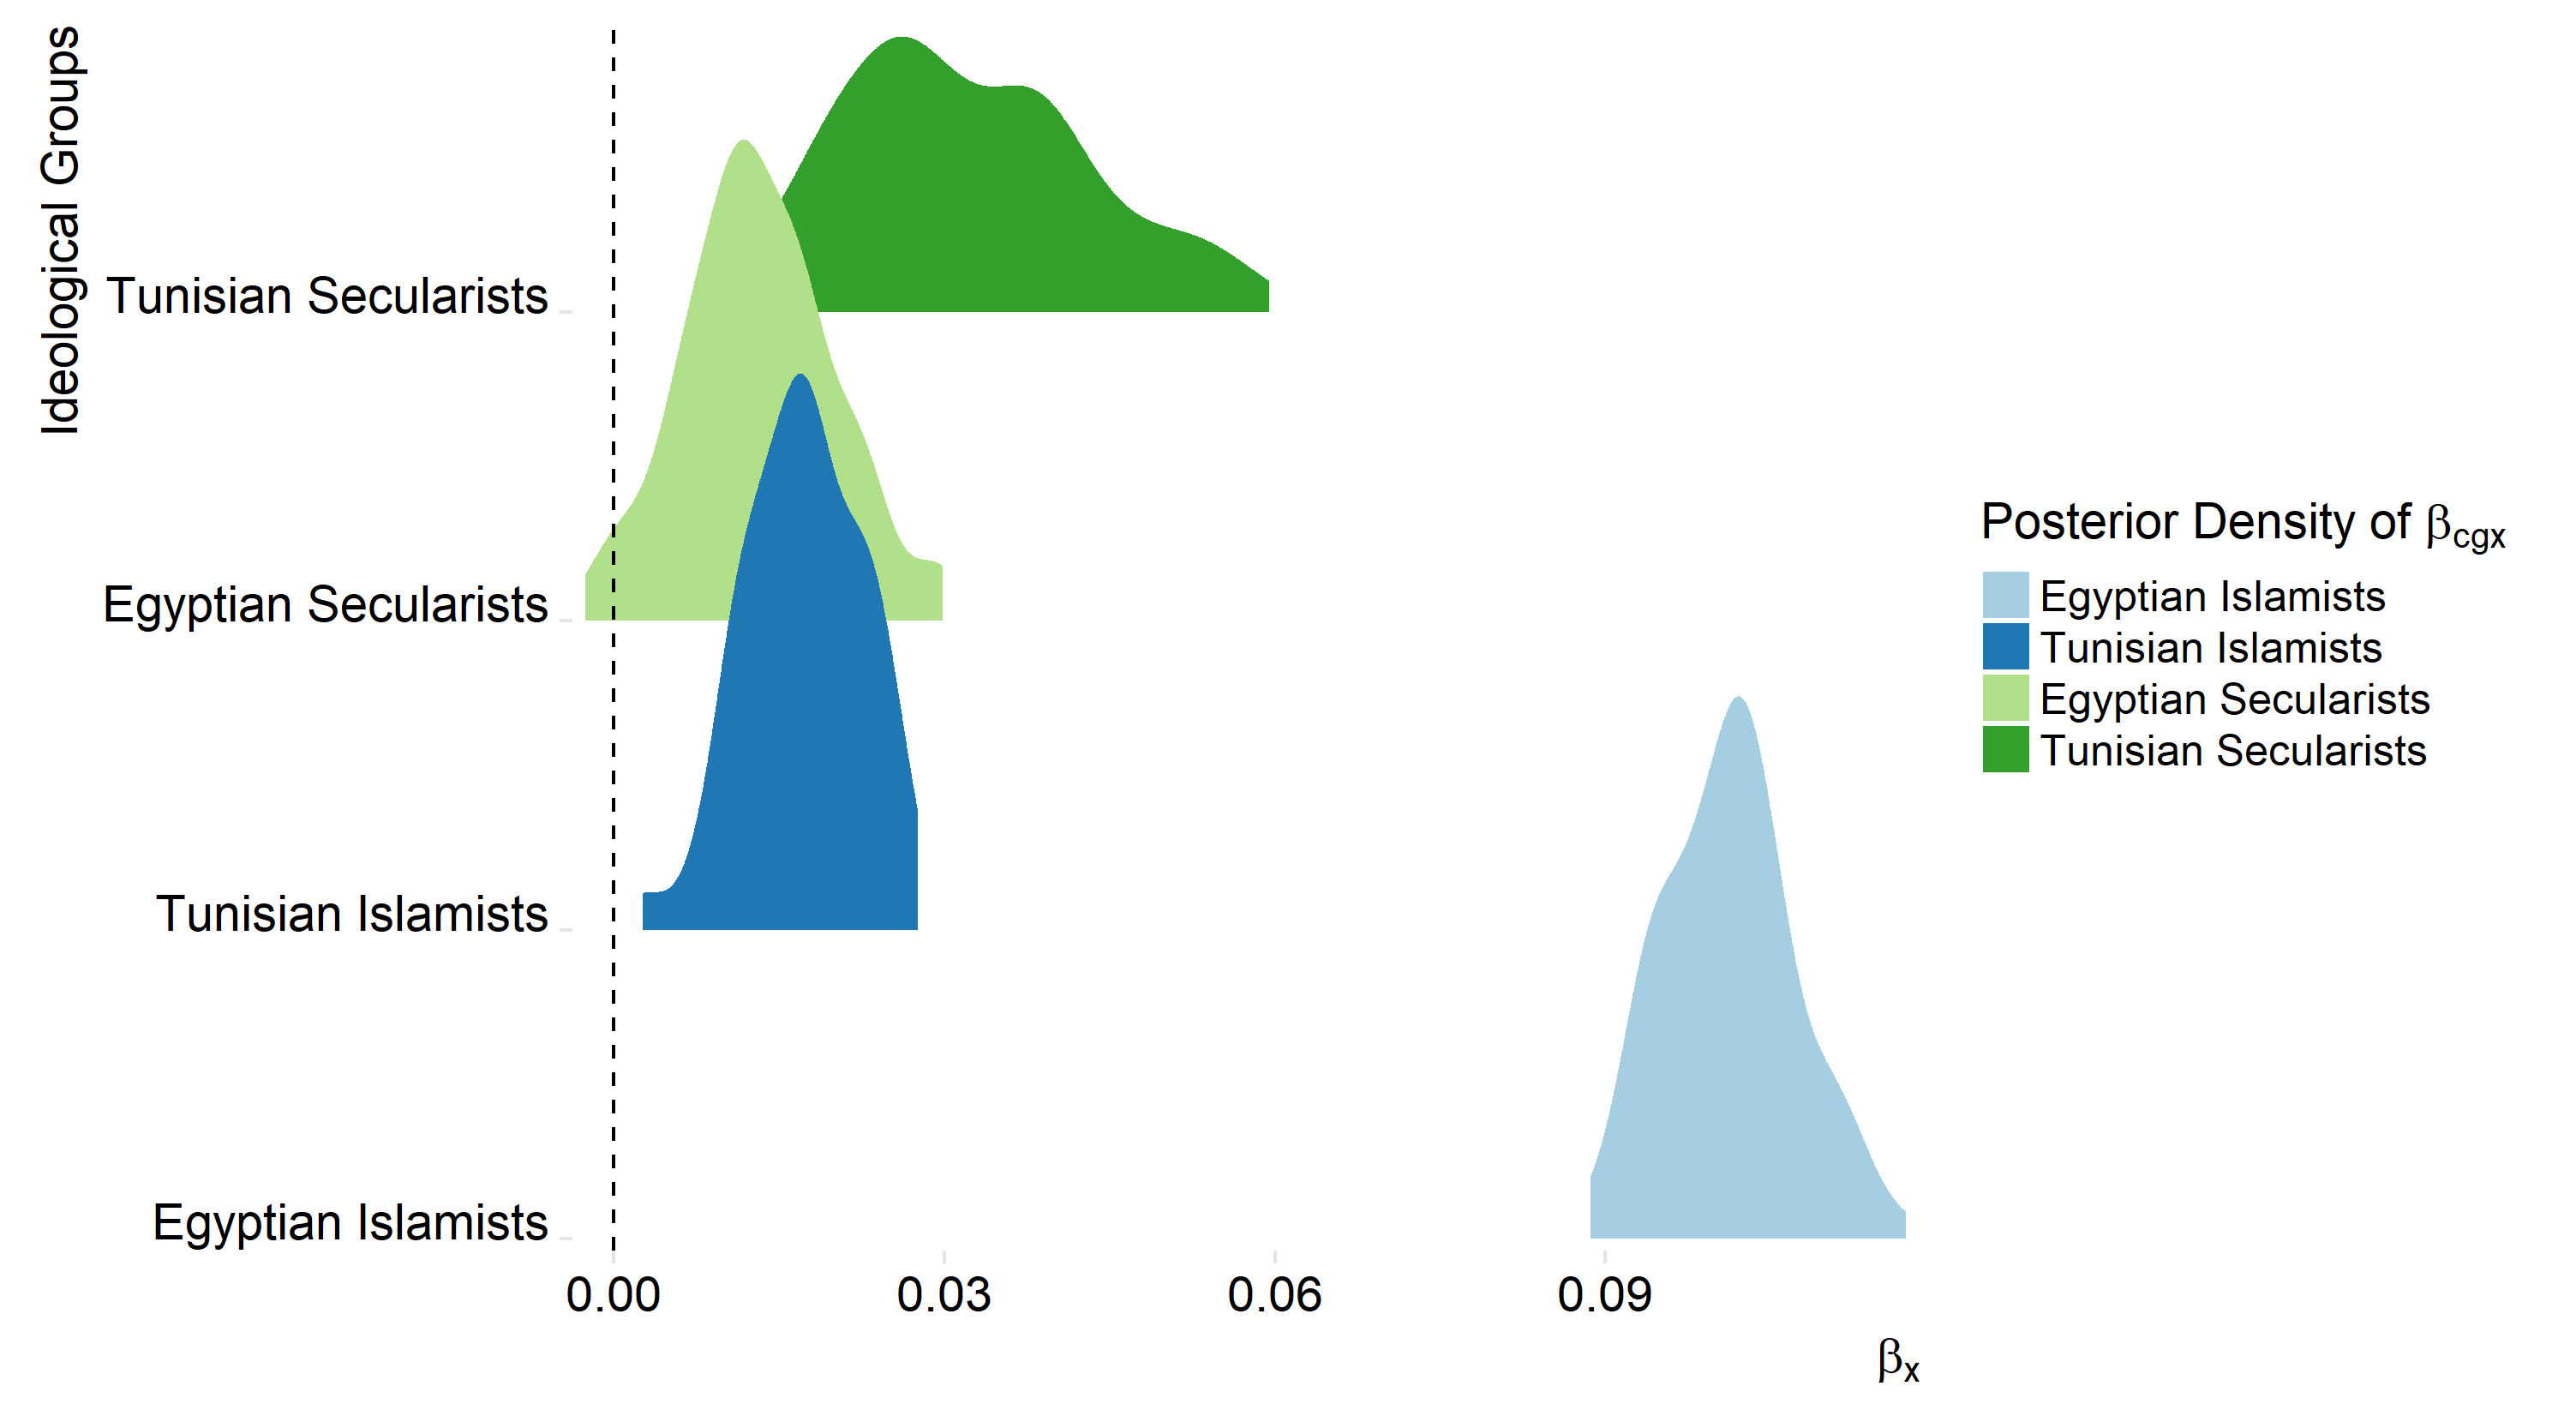
\includegraphics[width=.9\linewidth]{betax}
\end{figure}

The values of the $\beta_{cgOUT}$, on the other hand, allow us to make statements about how each group is influenced by its foreign ideological allies. Of these parameters, Egyptian Islamists and Tunisian secularists have the highest absolute value. Egyptian secularists, on the other hand, have a rather small though very precisely estimated influence from Tunisian secularists. In general, it is clear that Islamists are influenced to a greater extent by foreign allies than are secularists.

In addition to these diagnostic parameters, we can also look at direct measures of polarizing events. Figure \ref{betax} shows the posterior densities for our $\beta_{cgx}$ parameter that measures the total effect of Morsi's coup on each of the time series. As can be seen, these values are uniformly positive and statistically distinguishable from zero. Unsurprisingly, the effect on Egyptian Islamists is significantly larger than for other groups. To interpret these values correctly, the relative position of each ideological group in Figure \ref{arab_id_facet} must be kept in mind. Because Egyptian secularist are further down the scale than Egyptian Islamists, the positive values imply that 1) Egyptian Islamists moved away from Egyptian secularists after the coup and that 2) to a much lesser extent, Tunisian Islamists shifted away from Egyptian Islamists. Interestingly, the coup pushed Tunisian secularists closer to their ideological allies in Egypt, while the coup did not appear to have any direct effect on Egyptian secularists. 

While these interpretations are substantively interesting, the value of $\beta_{cgx}$ alone cannot answer the questions posed by our hypotheses because these static values do not capture feedback effects or time auto-correlation. To test our hypotheses precisely, we calculate the impulse-response functions (IRFs) mentioned previously to test the hypotheses in Table \ref{Htests}. First, we examine H1 in Figure \ref{cross_irf}, which involves testing a basic null hypothesis that we should be able to detect some kind of response in one ideological group from a unit shock to their foreign ideological allies. While this shock is substantively quite large, using a 1-unit shock is convenient as we can then interpret the y axis as representing the proportion of the shock that transfered from one country to another. As can be seen in Figure \ref{cross_irf}, a one-unit shock in a foreign ideological ally does result in movement in each group. Tunisian secularists show the greatest responsiveness, with more than 50\% of the shock transferring across borders in the initial day after the shock. Islamists in both countries see substantively large shock transfers between 10 and 20 percent. Secularists in Egypt see the smallest shock transfer at between 1 and 3 percent.
 \begin{figure}[!h]
	\centering
	\caption{IRF for 1-Unit Shock from Transnational Ideological Groups}\label{cross_irf}
	\centering
	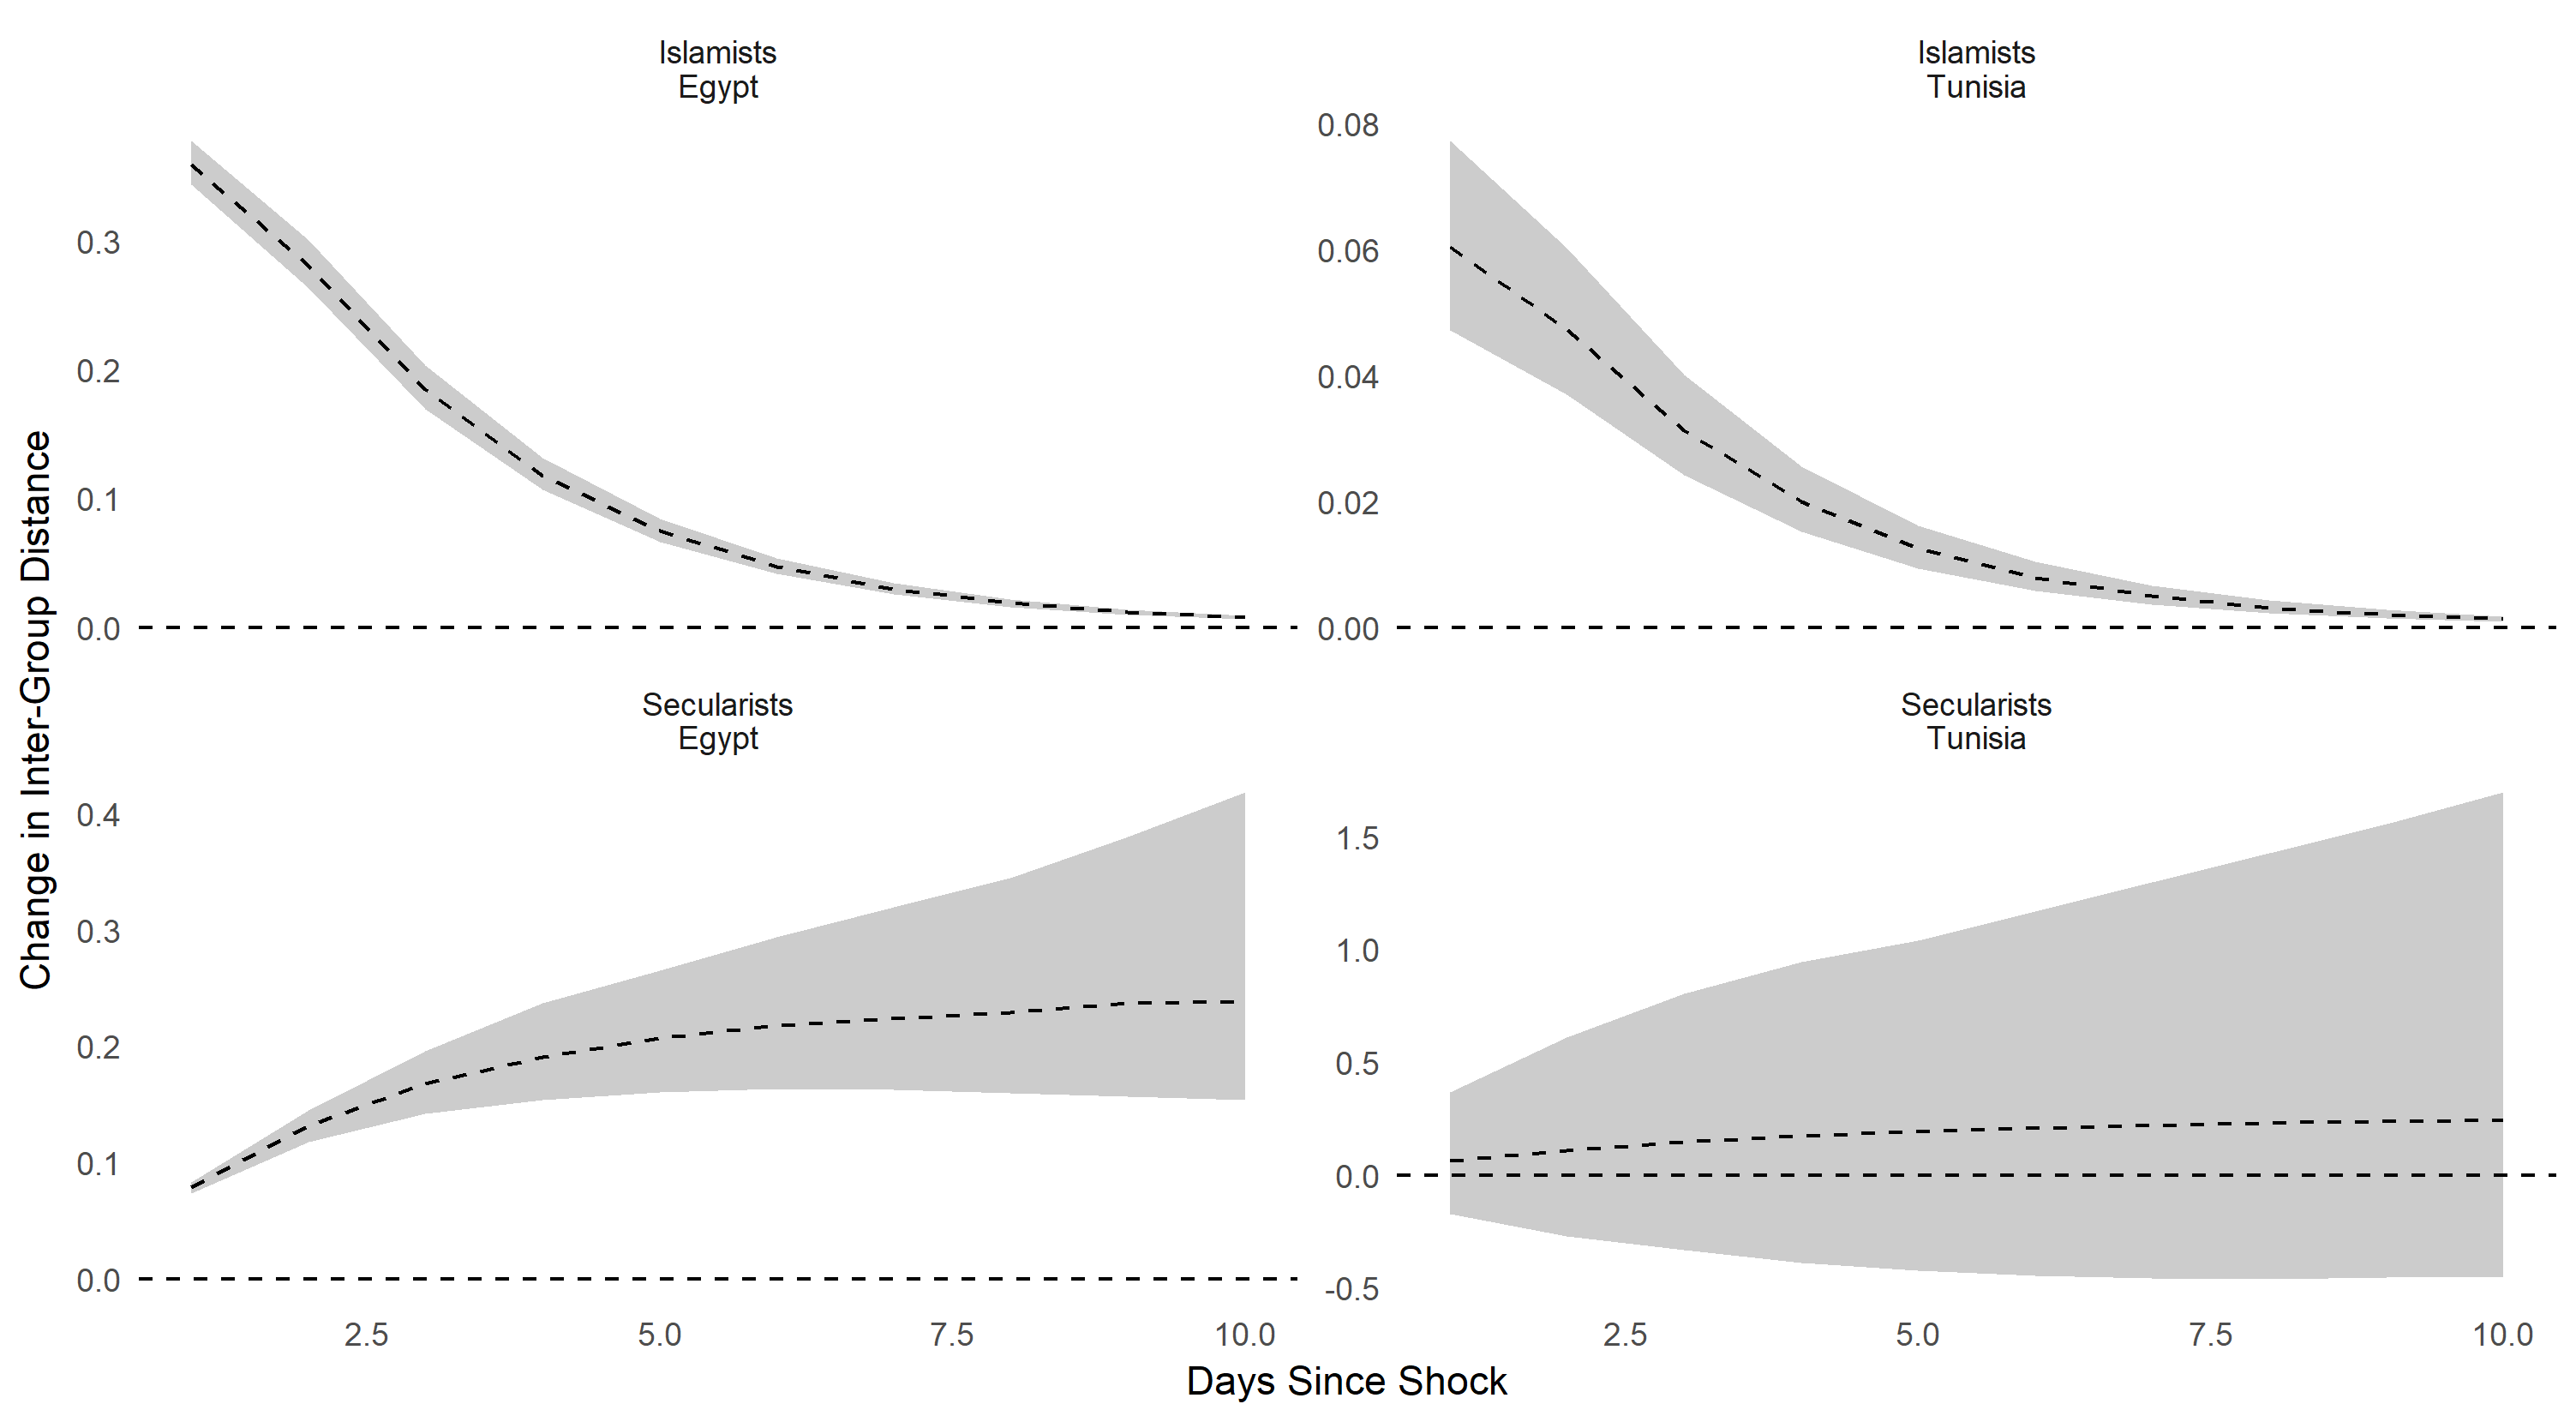
\includegraphics[width=.9\linewidth]{irf_egypt_panels}
\end{figure}

To test hypothesis 2, we can employ the same IRF technique except now we use the estimates for the Morsi coup effect $\beta_{cgx}$ instead of a hypothetical 1-unit shock. In hypothesis 2, we are testing for the direct effect; i.e., whether the coup had a statistically distinguishable effect on each ideological group on itself over time. Figure \ref{within_betax} reveals that this direct effect does generally exist. Substantively, all ideological groups have a quick response to the coup, with the exception of secularists in Egypt, who have a relatively precisely estimated null effect. It is interesting again to note that the signs of the effect among Islamists will tend to push them apart in the immediate aftermath of the coup.
 \begin{figure}[!h]
	\centering
	\caption{IRF for Within-Time Series Direct Effect of Coup $\beta_{cgx}$}\label{within_betax}
	\centering
	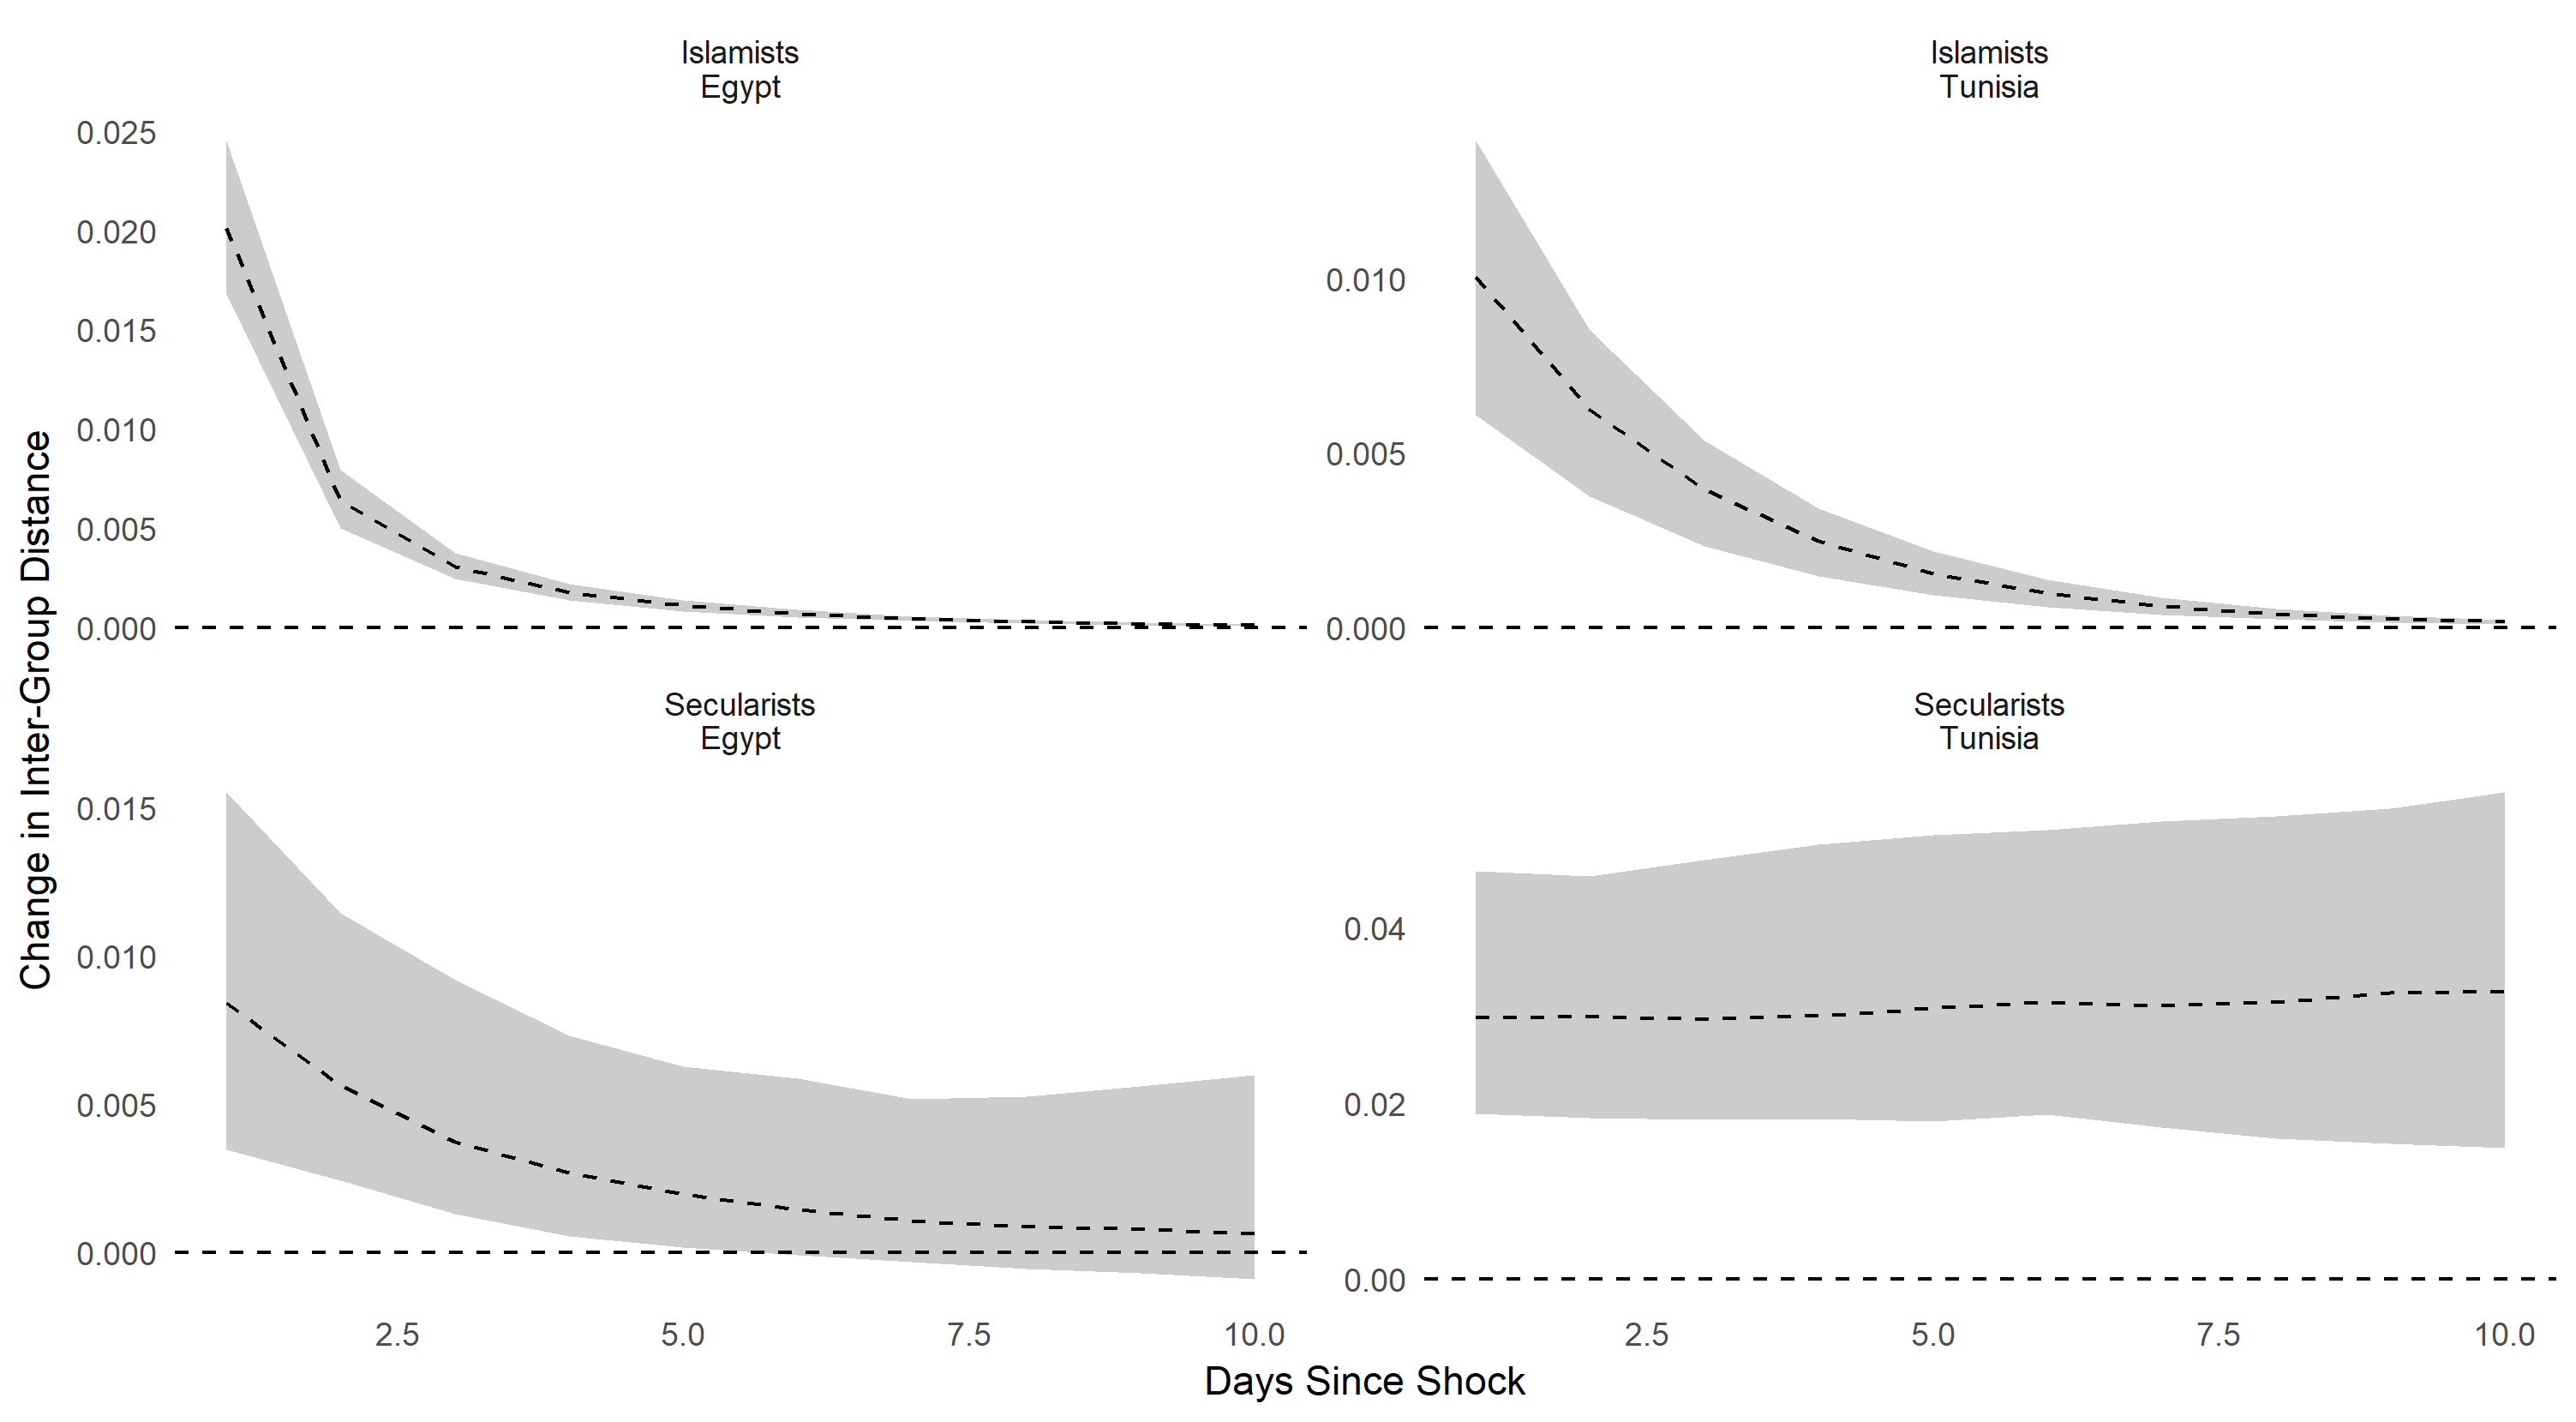
\includegraphics[width=.9\linewidth]{irf_betax_within}
\end{figure}

Next we test the indirect effect mentioned in hypothesis 3 of the Morsi coup, or the amount with which the shock of the coup transferred to ideological allies, in Figure \ref{indirect_betax}. Surprisingly, these effects are as large or larger in some cases than the direct effects in Figure \ref{within_betax}. Interestingly, the indirect effects of Egyptian and Tunisian Islamists are almost identical because the smaller direct effect for Tunisian Islamists counterbalances Egyptian Islamists' greater sensitivity to transnational polarization. Again, we would note that the shock decays much more slowly among secularists due to their relatively less stable position in the system. Overall, the evidence shows that there are indeed indirect feedback effects of the coup across countries for ideological groups, but especially for Islamists.
 \begin{figure}[!h]
	\centering
	\caption{IRF for Within-Time Series Indirect (Transnational) Effect of Coup $\beta_{cgx}$}\label{indirect_betax}
	\centering
	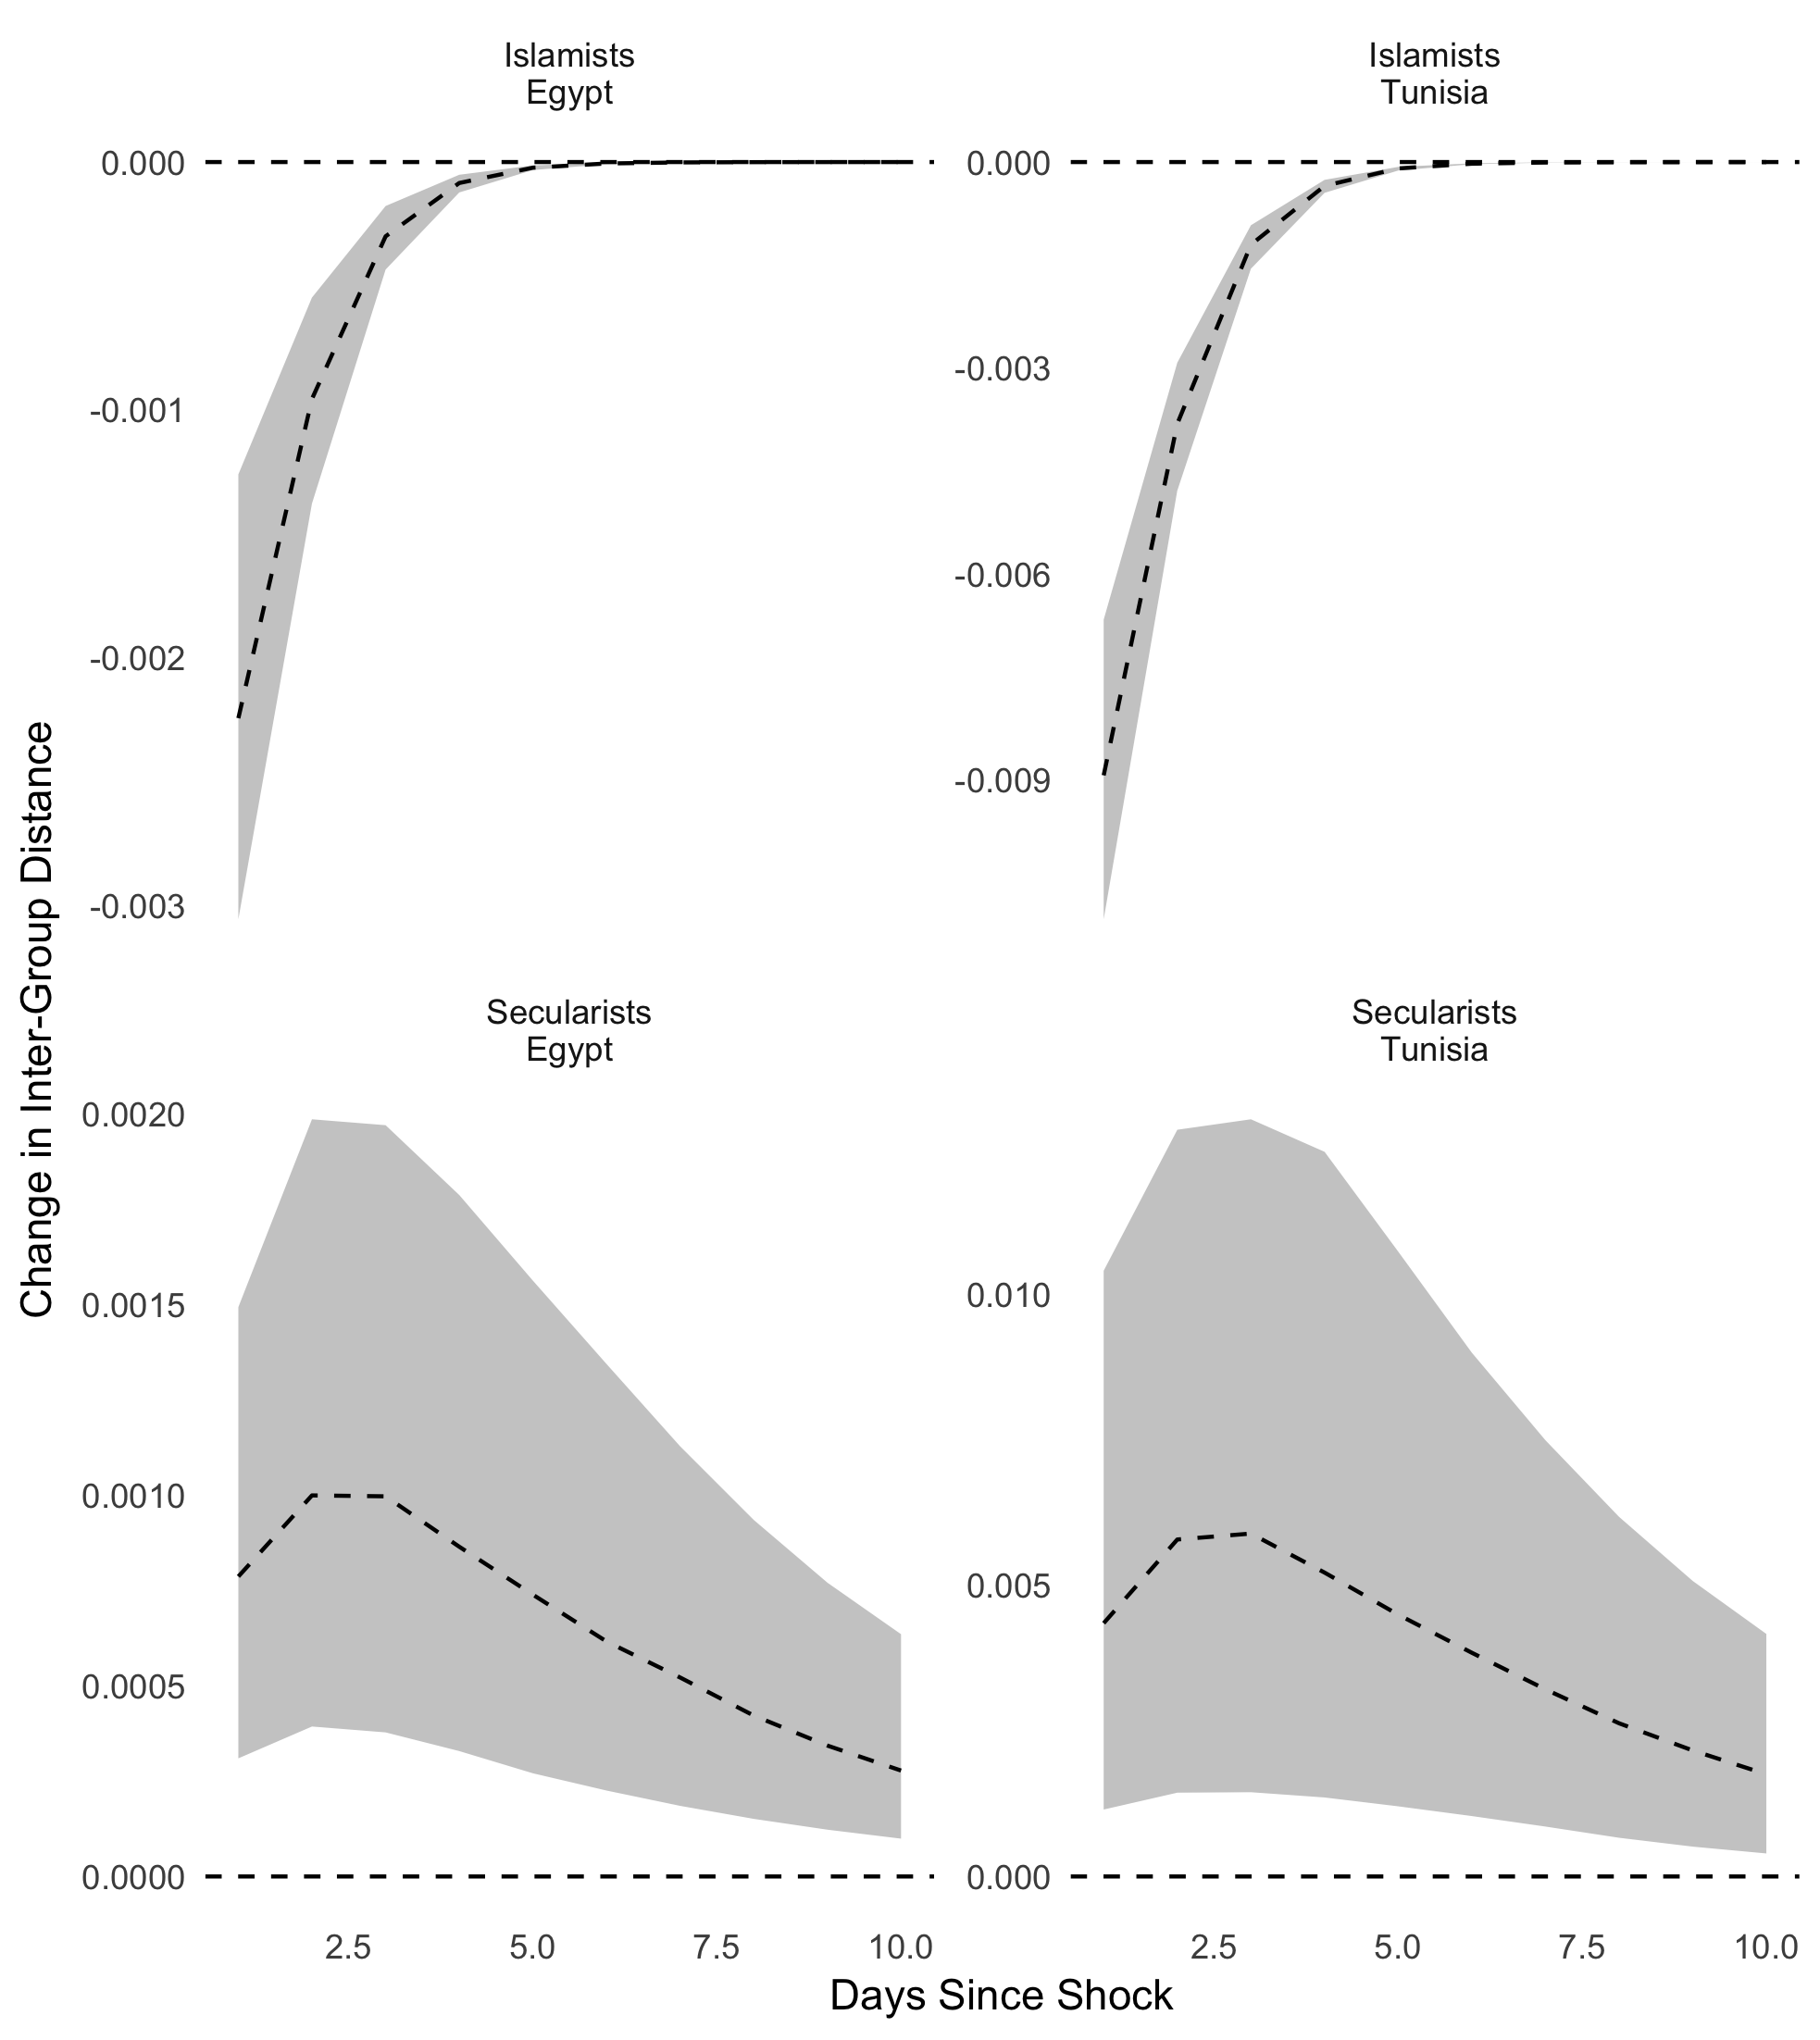
\includegraphics[width=.9\linewidth]{irf_betax_other}
\end{figure}
 \begin{figure}[!h]
	\centering
	\caption{IRF for Within-Time Series Combined Effect of Coup $\beta_{cgx}$}\label{combine_betax}
	\centering
	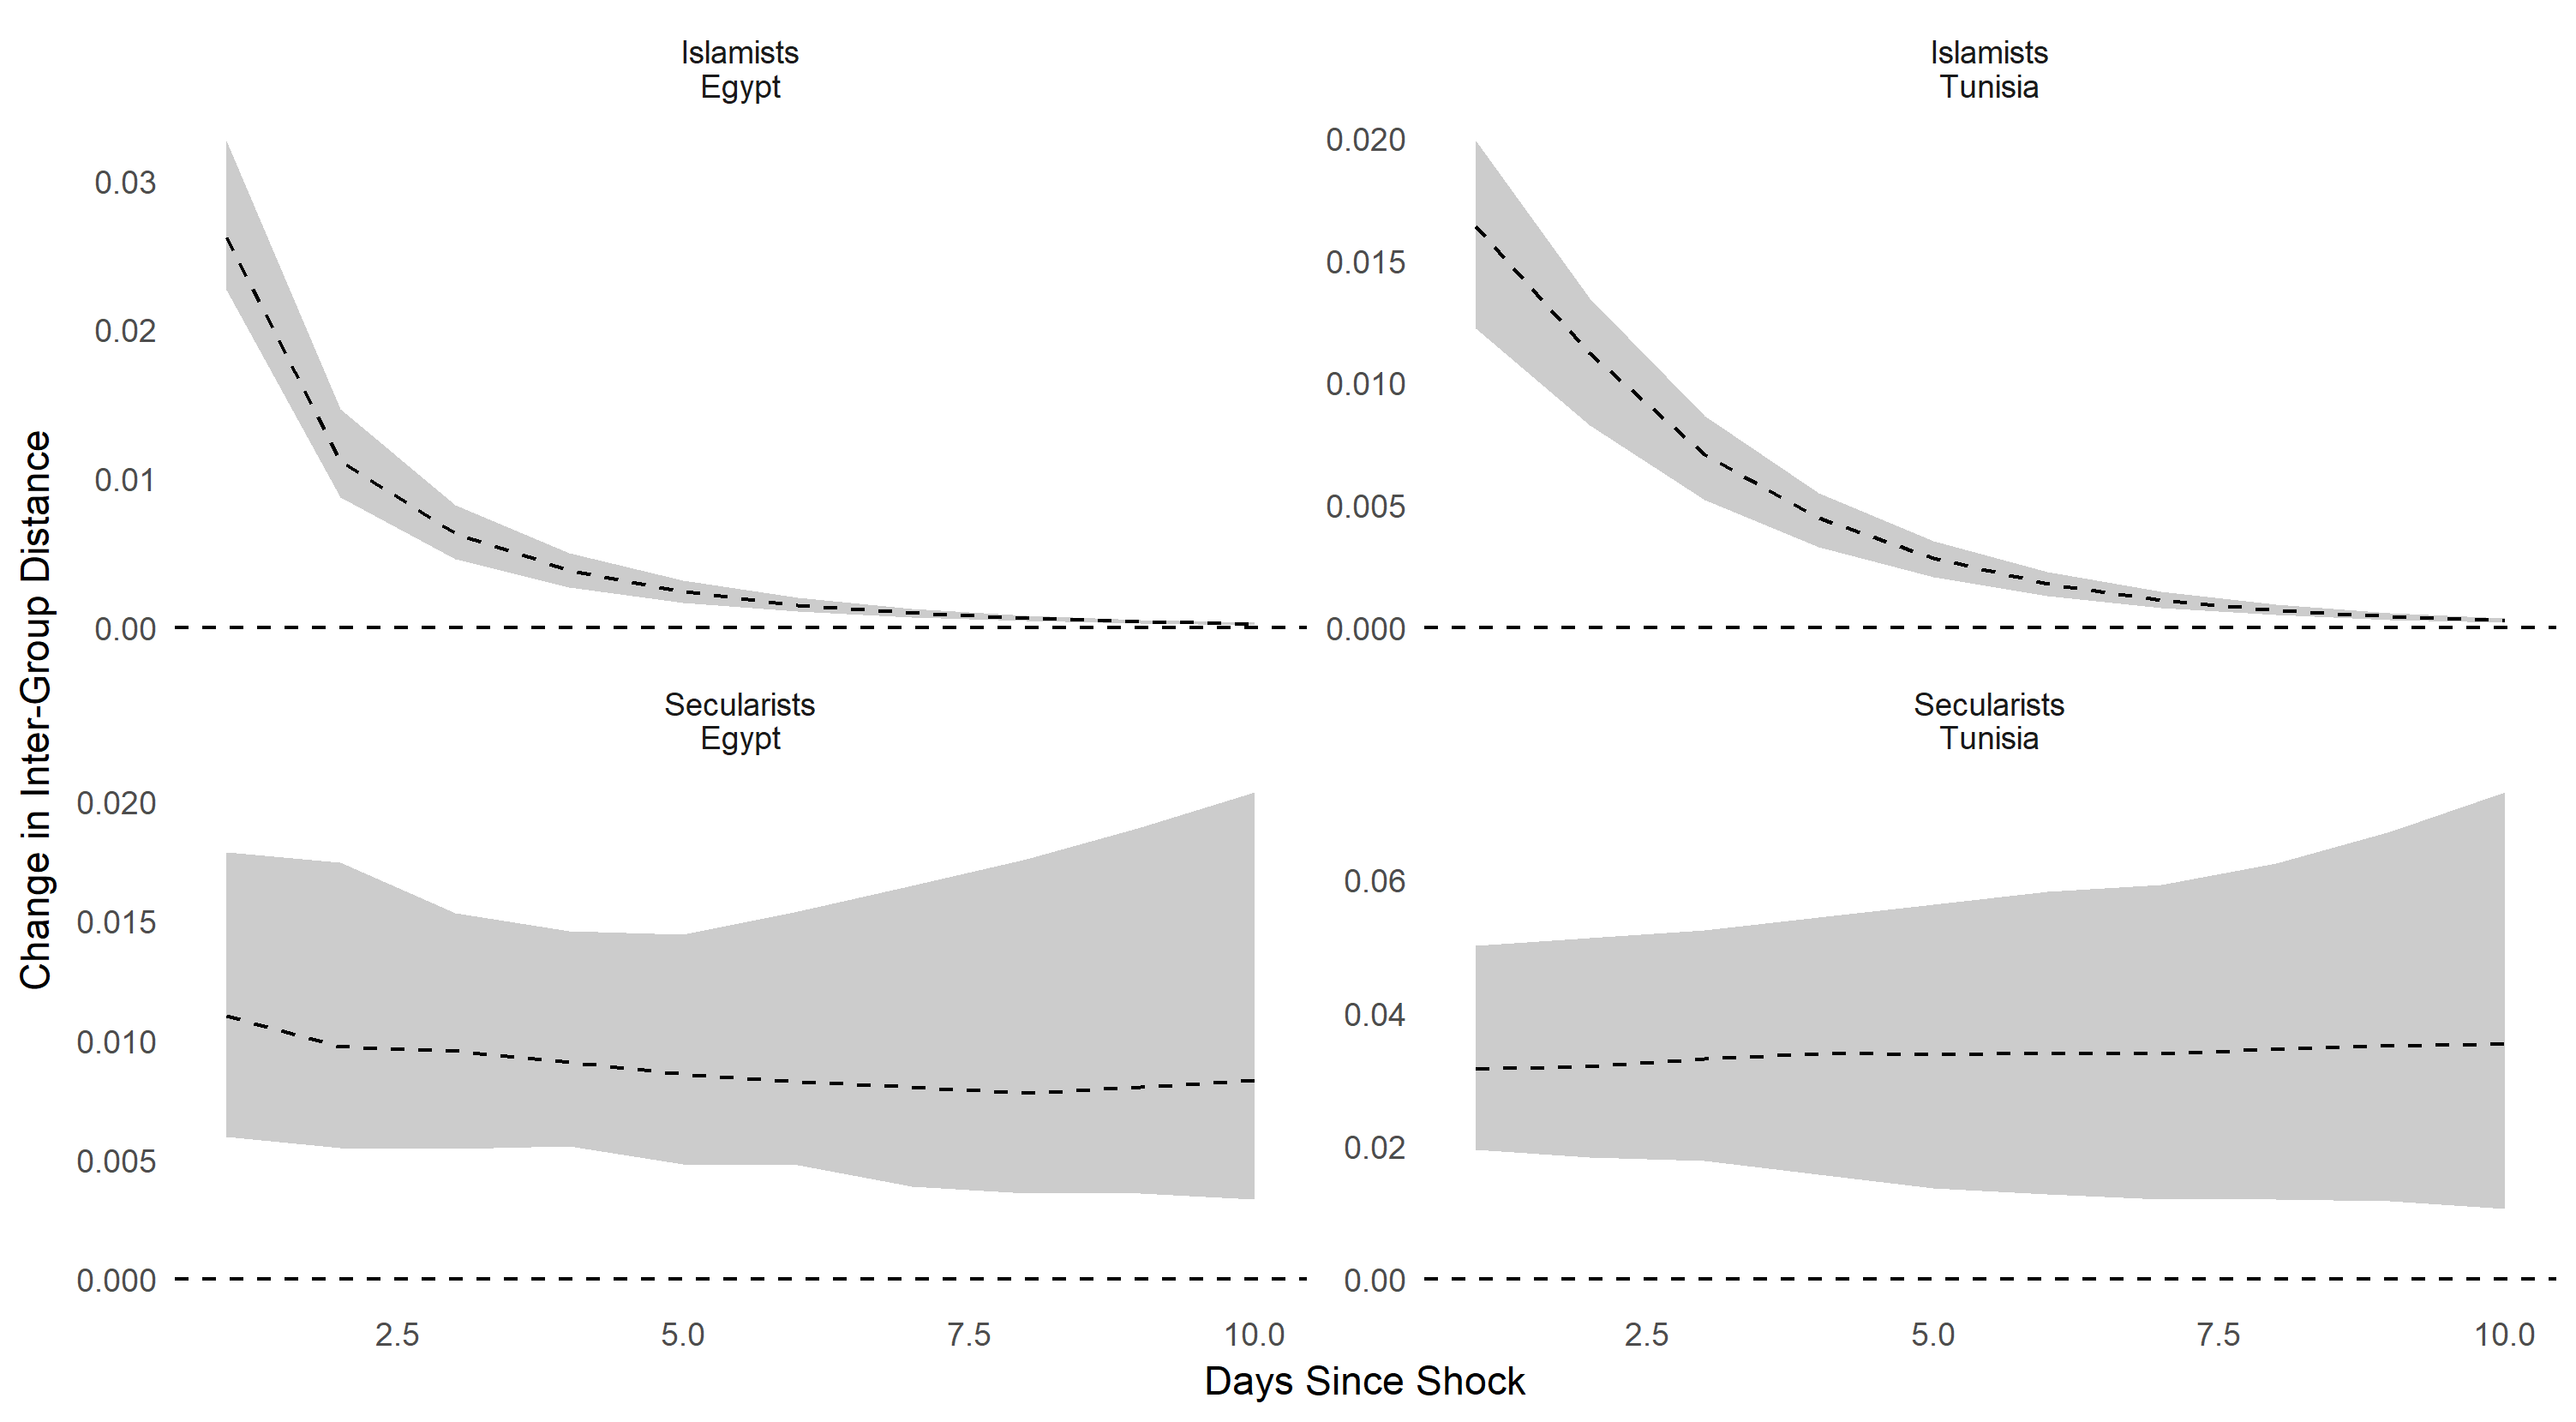
\includegraphics[width=.9\linewidth]{irf_betax_both}
\end{figure}
 \begin{figure}[!h]
	\centering
	\caption{Comparison of IRF for Direct and Combined Effect of Coup $\beta_{cgx}$}\label{compare_betax}
	\centering
	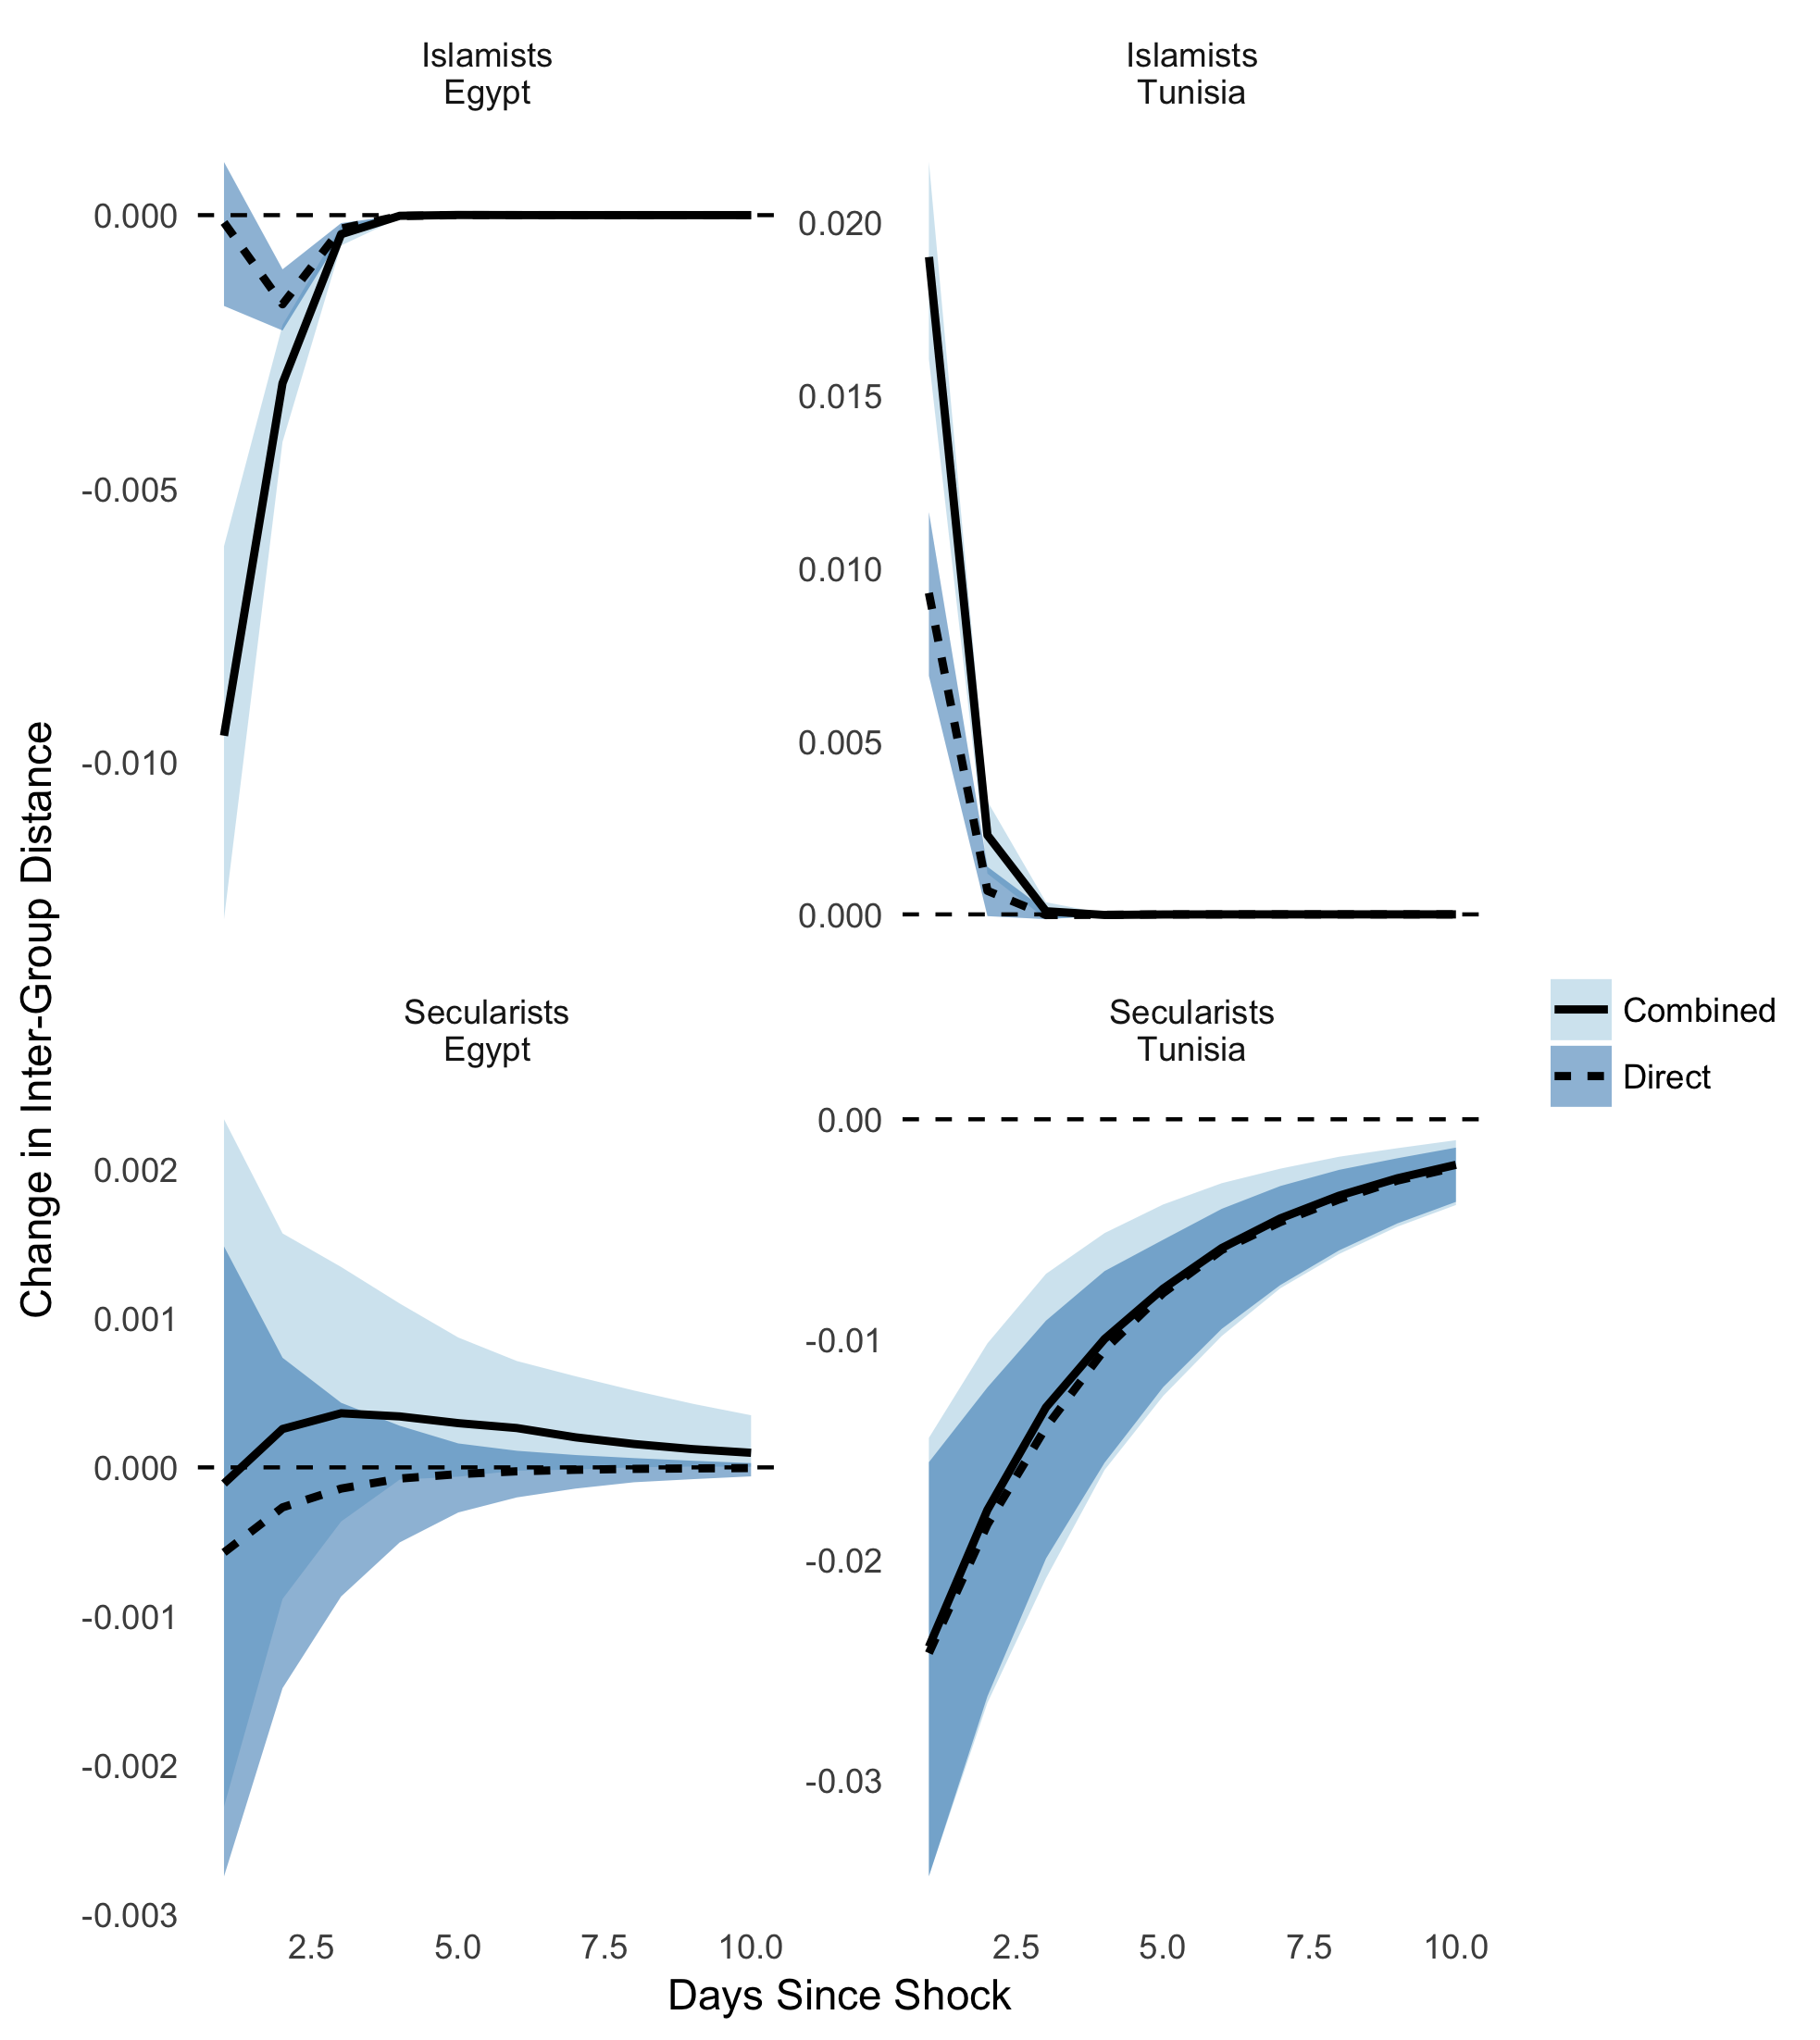
\includegraphics[width=.9\linewidth]{irf_betax_compare}
\end{figure}

Finally, we examine hypothesis 4, which proposes that the combined effect of both the direct and indirect effects of the coup will also be positive. In other words, once cross-border polarization is taken into account, the coup actually has a greater total effect on moving the inter-group distance of ideological groups within countries. This hypothesis could be falsified if the direct and indirect effects counterbalanced each other, but as Figures \ref{combine_betax} and \ref{compare_betax} reveal, the combined effect is indeed greater than either the indirect or direct effect for Islamists, although there is no statistically distinguishable difference for secularists. This difference can be seen by overlaying the combined effects on the direct effects, which we do in Figure \ref{compare_betax}. This plot makes the point that for Islamists, the combined feedback effects serve to increase their movement in the latent space, while for secularists, this is not necessarily so. Secularists in Tunisia are largely indifferent to movement in their foreign ideological allies, while for secularists in Egypt, their co-religionists response to the coup does heighten their own response relative to the direct effect, although the difference is not very precise. In all, it is clear that the combined effects, or both the within-group effect of the coup and the feedback traveling across borders, prompt a higher level of salience and movement in the ideological space that corresponds to our theory of how ideological groups receive and transmit transnational polarization. However, this finding exists only for Islamists, while secularists tend to be relatively unaffected by the polarization of their ideological allies. Secularists still respond to sectarian shocks, but the channels for polarization are not primarily transnational but rather intranational.


\section*{Discussion}

Because both the model, theory and data in this paper are novel, the external validity of this analysis is limited. We have not been able to measure this kind of ideological polarization so precisely, and so we do not know whether the results we observe are substantively large relative to the universe of transnational sectarian polarization. Thus as is often the case, the increase in measurement precision also generates new hypotheses and areas for exploration, and one of the main avenues for future inquiry is to apply this model to other countries, ideological groups, and time periods. 

This study is further limited by the time range under consideration, approximately nine months during a period of political instability in the Arab Spring. As we described in our theory section, endogenous polarization occurs within and between countries over time, so it can be difficult to obtain a long enough series to show all of the polarizing effects and their consequential after-shocks. For our data, we are limited in modeling dynamics before 2012 because many of the Islamists did not open Twitter accounts until the beginning of 2013, leaving limited ideological diversity prior to that date. This limited time series may explain why we do not observe an even larger polarizing effect of Morsi's coup: by the beginning of 2013, groups had already become polarized, which would leave less room for yet more polarization to occur.

Yet even with those two previous caveats, our findings provide important insight into the underlying dynamics of transnational ideological polarization occurs. It is difficult to study endogenous processes whether qualitatively or quantitatively, and we are able to analyze a very large dataset and reduce it down to the particular latent social cleavage of interest. Given how responsive the inter-group distance measure is to clearly polarizing events--some of which we did not identify in advance, such as the draft Tunisian constitution--our model's internal validity appears quite high.

As a result, the precision of the hypotheses tests we are able to implement in this paper enable us to identify the direct, indirect and combined \emph{transnational} effects of inter-group polarization. Being able to separate these different components of the feedback process allows us to substantiate the major elements of the theory, and to support the central point of our paper that transnational linkages among ideological groups can endogenously heighten polarization independent of what is occurring within that group's country. While we are not the first to document such linkages, we are the first to directly measure this kind of transnational ideological polarization in a way that incorporates our uncertainty in measuring latent social cleavages.

Our analysis also raises questions that we had not considered before. The surprisingly higher instability of secularists' ideal points, measured by the rate at which their time series returned to a long-term mean, indicates that secularists were relatively less entrenched in this latent space in terms of their sectarian identity. Islamists, by contrast, and Egyptians in particular, were much more rigidly defined. It is perhaps not surprising, then, that Islamists also show much higher levels of sensitivity to movement in each other's ideal points relative to secularists.

We would note as well that this polarization of foreign allies did not always result in additional within-country polarization. Tunisian Islamists and secularists seemed to move closer to each other, at least when looking at their response to Morsi's coup. Although we cannot with complete certainty tie these dynamics to observed outcomes in these countries, it is interesting to note that Tunisians were more able to contain sectarian conflict and reach a political compromise in which the Islamist party stepped down for new elections, while sectarian conflict in Egypt resulted in brutal repression of Islamists that continues until today.

In addition, we believe that the time series estimates may also be affected by de-polarization. In Tunisia, Islamists were under considerable pressure during this time period as they faced rising unrest because of violence from Islamic radicals \parencite{mccarthy2016}. For that reason, post-coup they may have feared supporting their co-religionists too publicly lest they suffer a similar fate within their own country \parencite{grewal2016}. This kind of suppression may explain why Tunisian Islamists tended to move closer to Tunisian secularists in response to the coup and Egyptian Islamists' reaction, while the opposite occurred for Egyptian Islamists. 

We would note as well that an area for future research would be to incorporate an explicit second-dimension to ideological polarization, that of the pro and anti-democracy axis, perhaps through the use of compensatory multi-dimensional IRT \parencite{reckase2009}. We believe that this second dimension explains why the changes in the Tunisian constitution provoked a wider swing in inter-group distance than did Morsi's coup. Some secularists in both countries opposed the coup because of their commitment to democratic norms, which arguably reduced polarization or at least made it less likely for these secularists to adopt a more negative view of Islamists as a result of the coup. By comparison, the constitutional changes in Tunisia did not divide secularists along a democratic axis, which more cleanly activated the secularist-Islamist cleavage. This difference between the two events is further validation for our method of identifying the secularist-Islamist cleavage, but future work could examine more closely how cleavages interact with each other. A challenge to accomplish this is to find a way to effectively code pro and anti-democratic views as there is a strong social desirability bias against expressing anti-democratic opinions, even in authoritarian countries.

One area of our data that we have not explored is the content of the tweets themselves. In fact, our empirical strategy is based in part on avoiding the challenging task of parsing tweets into useful categories. However, our approach to grounding the model in assigned ideological labels and retweets provides an avenue for incorporating text. A major challenge in text analysis is to know how to identify latent variables of interest underlying word counts \parencite{slapin2008,grimmer2013}. By incorporating coded labels and retweets as a relatively direct measure of polarization, text can then be included as an additional source of information about polarization. This approach is similar to the recent efforts to find ways of estimating ideal points for legislators that combine both the text of legislation and legislators' observed votes \parencite{lauderdale2014}. For these reasons, our model does not preclude analysis of text but rather helps provide an estimation framework for sifting through the noise in Twitter content.

\section*{Conclusion}

In this paper we put forward a method of estimating the latent positions of ideological groups in Egypt and Tunisia during the tumultuous period of the Arab Spring. We take advantage of Twitter's widespread usage to show how latent ideological scores change over time and also in tandem with similar ideological groups in other countries. The use of the IRT-VAR model allows for these estimates to incorporate measurement uncertainty while also providing useful summary measures of inter-group distance.

We find that the overthrow of Mohammed Morsi in a coup by the Egyptian military resulted in a long-term shift of the latent social cleavages of both secularists and Islamists in Egypt. This shock also eventually resulted in both groups moving farther apart from each other in the months ahead. The aftermath of the coup had its greatest effect on shifting the ideal points of Egyptian and Tunisian Islamists, with weaker effects on Egyptian and Tunisian secularists. Furthermore, we find that the combined effect of both the coup on the Islamists along with the feedback each group received from its foreign ideological ally resulted in greater movement in ideal points among Islamists, and hence polarization, but the same did not hold for secularists. 

This research opens the door to further exploration of the determinants and measurement of ideological polarization during periods of political instability. This model provides a rich range of estimates and can pinpoint places at which polarizing events occurred. Furthermore, we can show how short-term shocks translate into long-term differences in idealogical polarization over time. We hope that this evidence stimulates more investigation of the determinants and effects of group feedback effects in ideologically-polarized societies.

\section*{Appendix A: List of Elites}

% latex table generated in R 3.4.3 by xtable 1.8-2 package
% Wed May 30 16:04:59 2018
\begin{longtable}{ll}
  \toprule
Username & Secularist/Islamist \\ 
  \midrule
slim404 & Secularist\_Tunisia \\ 
  ooouups & Secularist\_Tunisia \\ 
  nawaat & Secularist\_Tunisia \\ 
  psycke & Secularist\_Tunisia \\ 
  karim2k & Secularist\_Tunisia \\ 
  riadheh & Secularist\_Tunisia \\ 
  mira404 & Secularist\_Tunisia \\ 
  yassayari & Islamist\_Tunisia \\ 
  sarah\_bh & Secularist\_Tunisia \\ 
  majdikhan & Secularist\_Tunisia \\ 
  maramirou & Secularist\_Tunisia \\ 
  marwen & Secularist\_Tunisia \\ 
  benmhennilina & Secularist\_Tunisia \\ 
  slimazzabi & Secularist\_Tunisia \\ 
  jnayna & Secularist\_Tunisia \\ 
  azyyoz & Secularist\_Tunisia \\ 
  arabasta1 & Secularist\_Tunisia \\ 
  zinga\_ & Secularist\_Tunisia \\ 
  c\_moii & Secularist\_Tunisia \\ 
  jasmintn & Secularist\_Tunisia \\ 
  sans\_url & Secularist\_Tunisia \\ 
  indigo\_light & Secularist\_Tunisia \\ 
  takriz & Secularist\_Tunisia \\ 
  sameh\_b & Secularist\_Tunisia \\ 
  nayzek & Secularist\_Tunisia \\ 
  liliopatra & Secularist\_Tunisia \\ 
  eyaturki & Secularist\_Tunisia \\ 
  faiyla & Secularist\_Tunisia \\ 
  zizoo & Secularist\_Tunisia \\ 
  houeida & Secularist\_Tunisia \\ 
  malekk & Secularist\_Tunisia \\ 
  ahlemhc & Secularist\_Tunisia \\ 
  tom\_z & Secularist\_Tunisia \\ 
  chiheb12 & Secularist\_Tunisia \\ 
  zeinebturki & Secularist\_Tunisia \\ 
  khamousss & Islamist\_Tunisia \\ 
  may\_mouna & Secularist\_Tunisia \\ 
  yamenbousrih & Secularist\_Tunisia \\ 
  ifikra & Secularist\_Tunisia \\ 
  blech\_klem & Secularist\_Tunisia \\ 
  emnachebaane & Secularist\_Tunisia \\ 
  bidules & Secularist\_Tunisia \\ 
  khalilbm & Secularist\_Tunisia \\ 
  boukornineblog & Secularist\_Tunisia \\ 
  out\_\_rage & Secularist\_Tunisia \\ 
  yhzami & Secularist\_Tunisia \\ 
  viagramoniak & Secularist\_Tunisia \\ 
  mounej & Secularist\_Tunisia \\ 
  maroo\_king & Secularist\_Tunisia \\ 
  kiffegrave & Secularist\_Tunisia \\ 
  albawsalatn & Secularist\_Tunisia \\ 
  nizarus & Secularist\_Tunisia \\ 
  r\_ghannouchi & Islamist\_Tunisia \\ 
  nahdhatunisie & Islamist\_Tunisia \\ 
  ali\_larayedh & Islamist\_Tunisia \\ 
  yusraghkh & Islamist\_Tunisia \\ 
  ziedladhari & Islamist\_Tunisia \\ 
  bassemloukil & Secularist\_Tunisia \\ 
  mehdi\_jomaa & Secularist\_Tunisia \\ 
  alaa & Secularist\_Egypt \\ 
  waelabbas & Secularist\_Egypt \\ 
  ghonim & Secularist\_Egypt \\ 
  nawaranegm & Secularist\_Egypt \\ 
  sandmonkey & Secularist\_Egypt \\ 
  elbaradei & Secularist\_Egypt \\ 
  zeinobia & Secularist\_Egypt \\ 
  3arabawy & Secularist\_Egypt \\ 
  amrmsalama & Secularist\_Egypt \\ 
  monasosh & Secularist\_Egypt \\ 
  kalimakhus & Secularist\_Egypt \\ 
  drbassemyoussef & Secularist\_Egypt \\ 
  gamaleid & Secularist\_Egypt \\ 
  salmaeldaly & Secularist\_Egypt \\ 
  yosrifouda & Secularist\_Egypt \\ 
  wael & Secularist\_Egypt \\ 
  monaeltahawy & Secularist\_Egypt \\ 
  alyaagad & Secularist\_Egypt \\ 
  galalamer & Secularist\_Egypt \\ 
  amrwaked & Secularist\_Egypt \\ 
  mand0z & Secularist\_Egypt \\ 
  adel\_salib & Secularist\_Egypt \\ 
  hazem\_azim & Secularist\_Egypt \\ 
  ahmadesseily & Secularist\_Egypt \\ 
  zeinabsamir & Secularist\_Egypt \\ 
  lilianwagdy & Secularist\_Egypt \\ 
  5orm & Secularist\_Egypt \\ 
  sarahcarr & Secularist\_Egypt \\ 
  gsquare86 & Secularist\_Egypt \\ 
  minazekri & Secularist\_Egypt \\ 
  ahmednaguib & Secularist\_Egypt \\ 
  gemyhood & Secularist\_Egypt \\ 
  shokeir & Secularist\_Egypt \\ 
  heshoz & Secularist\_Egypt \\ 
  mennagamal & Islamist\_Egypt \\ 
  theboghdady & Secularist\_Egypt \\ 
  seksek & Secularist\_Egypt \\ 
  sarahngb & Secularist\_Egypt \\ 
  thebigpharaoh & Secularist\_Egypt \\ 
  h\_eid & Secularist\_Egypt \\ 
  lastoadri & Secularist\_Egypt \\ 
  rashapress & Secularist\_Egypt \\ 
  minanaguib90 & Secularist\_Egypt \\ 
  ahmad\_khalil & Secularist\_Egypt \\ 
  naguibsawiris & Secularist\_Egypt \\ 
  mazloum & Secularist\_Egypt \\ 
  nabilelhalfawy & Secularist\_Egypt \\ 
  alnagar80 & Secularist\_Egypt \\ 
  theadly & Secularist\_Egypt \\ 
  thesherio & Secularist\_Egypt \\ 
  kalnaga & Secularist\_Egypt \\ 
  midoo0 & Secularist\_Egypt \\ 
  dr\_heba\_raouf & Islamist\_Egypt \\ 
  moftasa & Secularist\_Egypt \\ 
  ahmdalish & Secularist\_Egypt \\ 
  theonlywarman & Secularist\_Egypt \\ 
  pakinamamer & Secularist\_Egypt \\ 
  zelaky & Secularist\_Egypt \\ 
  embee & Secularist\_Egypt \\ 
  ahmada2 & Secularist\_Egypt \\ 
  ramiii & Secularist\_Egypt \\ 
  mar3e & Secularist\_Egypt \\ 
  alaaaswany & Secularist\_Egypt \\ 
  alienzero & Secularist\_Egypt \\ 
  salmasaid & Secularist\_Egypt \\ 
  i3atef & Secularist\_Egypt \\ 
  loainagati & Secularist\_Egypt \\ 
  memam8 & Secularist\_Egypt \\ 
  ayaabdullah & Secularist\_Egypt \\ 
  bassem\_sabry & Secularist\_Egypt \\ 
  bothainakamel1 & Secularist\_Egypt \\ 
  tarekshalaby & Secularist\_Egypt \\ 
  m3adel & Secularist\_Egypt \\ 
  amrrodriguez & Secularist\_Egypt \\ 
  malek & Secularist\_Egypt \\ 
  etharkamal & Secularist\_Egypt \\ 
  ssirgany & Secularist\_Egypt \\ 
  \_\_safi\_\_ & Secularist\_Egypt \\ 
  hfakhry & Secularist\_Egypt \\ 
  hamzanamira & Islamist\_Egypt \\ 
  asmaamahfouz & Secularist\_Egypt \\ 
  egyptocracy & Secularist\_Egypt \\ 
  nasry & Secularist\_Egypt \\ 
  mohamedwaked & Secularist\_Egypt \\ 
  themiinz & Secularist\_Egypt \\ 
  muhammadmorsi & Islamist\_Egypt \\ 
  ikhwanweb & Islamist\_Egypt \\ 
  mushaweh & Islamist\_Egypt \\ 
  azzaelgarf & Islamist\_Egypt \\ 
  asmaaghazalll & Islamist\_Egypt \\ 
  alnourpartyeg & Islamist\_Egypt \\ 
  yonosmakhyoun & Islamist\_Egypt \\ 
  naderbakkar & Islamist\_Egypt \\ 
  gelhaddad & Islamist\_Egypt \\ 
  alqaradawy & Islamist\_Egypt \\ 
   \bottomrule
\end{longtable}


\section*{Appendix B: Simulation Study of IRT-VAR}


To construct the latent inter-group distance time series, we employ as our base specification the standard 2-PL IRT model that can be used to estimate the canonical ideal point model  \parencite{jackman2004}. Formally, we use this model to predict the mean of a product of Gaussian-distributed random variables $Y_{cgjt}$ (standardized retweet counts) with common variance $\sigma_Y$:

\begin{equation}\label{IRTbasic}
\prod^{c=1}_C \prod^{g=1}_G \prod^{j=1}_J \prod^{t=1}_T Y_{cgjt} \sim N( \delta_j  \alpha_{cgt},\sigma_{Y})
\end{equation}

In this model, $\alpha_{cgt}$ represent the latent ideal points of all the elites in each ideological group-country combination $gc$ at each time point $t$, while $\delta_j$ represents how strongly ideological citizen $j$'s retweet pattern is. We know from \textcite{jackman2004} that we can interpret this model as citizens choosing to retweet an elite if and only if that elite's ideal point in a latent space is closer to the citizen's ideal point in the latent space than the ideal point of any other elite. 

Given that we want to focus on relative changes in ideological polarization, we standardize $Y_{cgjt}$ within users so that the outcome represents the relative weight of each ideological group in a user's tweet patterns. This standardization helps us to address the problem that some users tend to retweet at much higher rates in general than other users \parencite{barbera2015}. It also significantly increases the speed of estimation relative to using a Poisson or other count model. However, for this reason we do not include intercepts as is normally the case in an IRT model because the standardization makes the intercepts equal to 0 by default \parencite{kropko2013}.

In order to estimate this model, we situate equation \ref{IRTbasic} in a Bayesian framework in which we define $\theta$ as the full set of parameters we can estimate in (\ref{IRTbasic}), and we want to know the most likely values of $\theta$ conditional on the observed data $Y_{cgjt}$:

\begin{equation}
p(\theta|Y_{cgjt}) \propto p(\theta)p(Y_{cgjt}|\theta)
\end{equation}

Using this standard form of Bayesian inference, equation \ref{IRTbasic} becomes the likelihood $p(Y_{cgjt}|\theta)$, and we can then look at endogenous relationships between ideal point parameters via the priors of these parameters, $p(\theta)$. In particular, building on \textcite{quinn2002} and \textcite{kropko2013}, we can model the vector auto-regression between the ideological groups $g$ via priors on the $\alpha_{cgt}$:

\begin{equation}\label{irtvar}
\alpha_{cgt}  \sim N(\gamma_{cg} + \beta_{cgIN}\alpha_{cg(t-1)} + \beta_{cgOUT}\alpha_{-cg(t-1)} + \beta_{gcx} X + \beta_c I(c),\sigma_{cg})\\
\end{equation}

Equation \ref{irtvar} shows how any one elite group $\alpha_{cgt}$'s latent score in time $t$ is a function of its prior time period latent score, $\beta_{cgIN}\alpha_{cg(t-1)}$, and the latent score of the same group $g$ but opposite country $-c$ in the previous time period, $\beta_{cgOUT}\alpha_{-cg(t-1)}$. As can be seen relative to equation \ref{var}, equation \ref{irtvar} substitutes the observed time series $y_t$ and $x_t$ with the latent ideal scores $\alpha_{cgt}$, but otherwise has the same parameters $\beta_{cgIN}$ and $\beta_{cgOUT}$. In other words, we use the IRT model to construct the time series by estimating the latent positions of the elite actors, but we are also able to directly estimate parameters of interest even with this measurement uncertainty. Because these priors are multiplied with the likelihood $p(Y_{cgjt}|\theta)$, we can then estimate a full joint density of both the IRT model and the vector autoregression between latent ideological positions so that uncertainty in both models is appropriately captured.

There are two other notable features of equation \ref{irtvar}. First, we include exogenous regressors $\beta_{gcx} X$ and $\beta_c I(c)$. $\beta_{gcx} X$ represents a binary vector that equals 0 before a polarizing event occurs, and 1 afterward, so that we can directly measure the effect of polarizing events on the ideal points $\alpha_{cgt}$. $\beta_c I(c)$ is an indicator function (dummy variable) that represents a fixed effect for countries and equals 1 when $c=Tunisia$ and 0 otherwise. We include this dummy variable as a way to help achieve identification of the rotation of the ideal points by constraining $\beta_c$ to be positive (see \parencite{gelman2005} for a full discussion of ideal point identification). Finally, we include separate variance parameters $\sigma_{cg}$ to directly model heteroskedasticity in the time series.

At this point, we have defined the IRT-VAR model that allows us to make time-series inferences on the over-time changes in the elite ideal points $\alpha_{cgt}$. However, this model is only defined over the retweet counts in which we have observed a citizen $j$ retweet one of the elites in a specific time period $t$. As mentioned in the previous section, we expand our observed data to include all the times that each citizen $j$ \emph{does not} retweet an elite in each time period, or $Y_{cgjt}=0$. If we simply include those zeroes in our likelihood $L(Y_{cgjt}|\theta)$ as additional data, we will be making the very strong assumption that each citizen $j$ looked at every tweet from every elite in time period $t$ and decided whether or not to retweet each tweet. In fact, that assumption may not hold for any of the citizens in our data except for unusually thorough citizens who want to have all influential Twitter users in their feed. As a result, we are concerned about a form of selection bias in which citizens are only exposed to tweets from those elites who are ideologically proximate to them, either because 1) Twitter's recommendation algorithm suggests that they follow elites who are ideologically proximate or 2) the citizen prefers to have a network is full of ideological allies or 3) both of these factors in interaction. 

For these reasons, we need a separate likelihood for the case when $Y_{cjgt}=0$. To do so, we incorporate the missing-data mechanism employed by \textcite{kubinec2017}, in which a hurdle model is used to account for missing data in an ideal point model when missingness is plausibly a function of the value of a person's ideal points. Given that this missingness pattern is very likely present in our data for the reasons previously described, we define a new likelihood $L(Y_{cjgt}=0|\lambda)$ conditional on a different set of parameters $\lambda$:

\begin{equation}
L(Y_{cjgt}=0|\lambda) = \prod^{c=1}_C \prod^{g=1}_G \prod^{j=1}_J  \prod^{t=1}_T logit^{-1}(\delta_{Aj}  \alpha_{cgt} - \eta_{Aj})
\end{equation}

What should be noted about this model is that we now have a Bernoulli-distributed random variable $Y_{cjgt}=0$, and so we predict this probability using a logit link function of the parameters in $\lambda$. These parameters represent a separate IRT equation with the same elite ideal points $\alpha_{cgt}$ but separate discrimination parameters for the citizens $\delta_{Aj}$. These separate set of citizen parameters represent a citizen's latent willingness to look at tweets from across ideological spectrum that is independent of that citizen's own individual ideal point, or what could be thought of as that citizen's desire to be informed of tweets from across the ideological spectrum. We include citizen intercepts $\eta_{Aj}$ that represent missingness that is ignorable, which will occur if $\delta_{Aj}=0$ and the probability of a citizen seeing a tweet is equal to that citizen's average number of tweets per group for the sample period. Ignorable missingness can occur if, for example, a citizen does not see tweets because they are working or on vacation. Importantly, in either case, the elite ideal points $\alpha_{cgt}$ that are our focus of inference will adjust to the uncertainty in this first-stage selection model. Our revised Bayesian model can then be written as follows in terms of the joint distribution of $Y_{cjgt}=0$, $Y_{cjgt}\neq0$, $\lambda$ and $\theta$:

\begin{align}
p(\theta,\lambda|Y_{cgjt}\neq0,Y_{cgjt}=0) \propto& p(\theta)p(\lambda) \cdot \\
&[ L(Y_{cgjt}=0|\lambda) + (1-L(Y_{cgjt}=0|\lambda))L(Y_{cgjt}\neq0|\theta)]
\end{align}

To finish our model specification, we include here our prior distributions for all other parameters in the model:

\begin{align}
\eta_{Aj} &\sim N(0,\sigma_{\eta})\\
\delta_j &\sim N(0,5) \\
\delta_{Aj} &\sim N(0,5) \\
\gamma_{cg} &\sim N(0,3)\\
\beta_{gcx} &\sim  N(0,3)\\
\beta_{cgIN} &\sim N(0,1)\\
\beta_{cgOUT} &\sim N(0,1)\\ 
\alpha_{cg1} &\sim N(0,1)\\
\sigma_{\eta} &\sim E(1)\\
\sigma_{cg} &\sim E(1)\\
\sigma_{\delta} &\sim E(1)
\end{align}

What is important to note about the prior distributions is that because the outcome is standardized, each standard deviation of 1 for a prior distribution corresponds to a standard deviation of 1 in the outcome if the prior has a Normal distribution. As such, the $N(0,3)$ and $N(0,5)$ represent weak priors, while the $\beta_{cgIN}$ and $\beta_{cgOUT}$ parameters receive stronger unit Normal priors in order to bias the model towards stationarity (although we do not impose a hard constraint). The hierarchical prior on $\eta_{Aj}$ is used for both regularization, as there are many citizens in the model, and for identification \parencite{gelman2005}. We also put a tight prior on the first time point of the elite ideal points $\alpha_{cg1}$ to help identify the scale of the ideal points.


\begin{figure}[!h]
	\caption{Recovery of True Impulse-Response Function Values}\label{irf_simulation_panels}
	\centering
	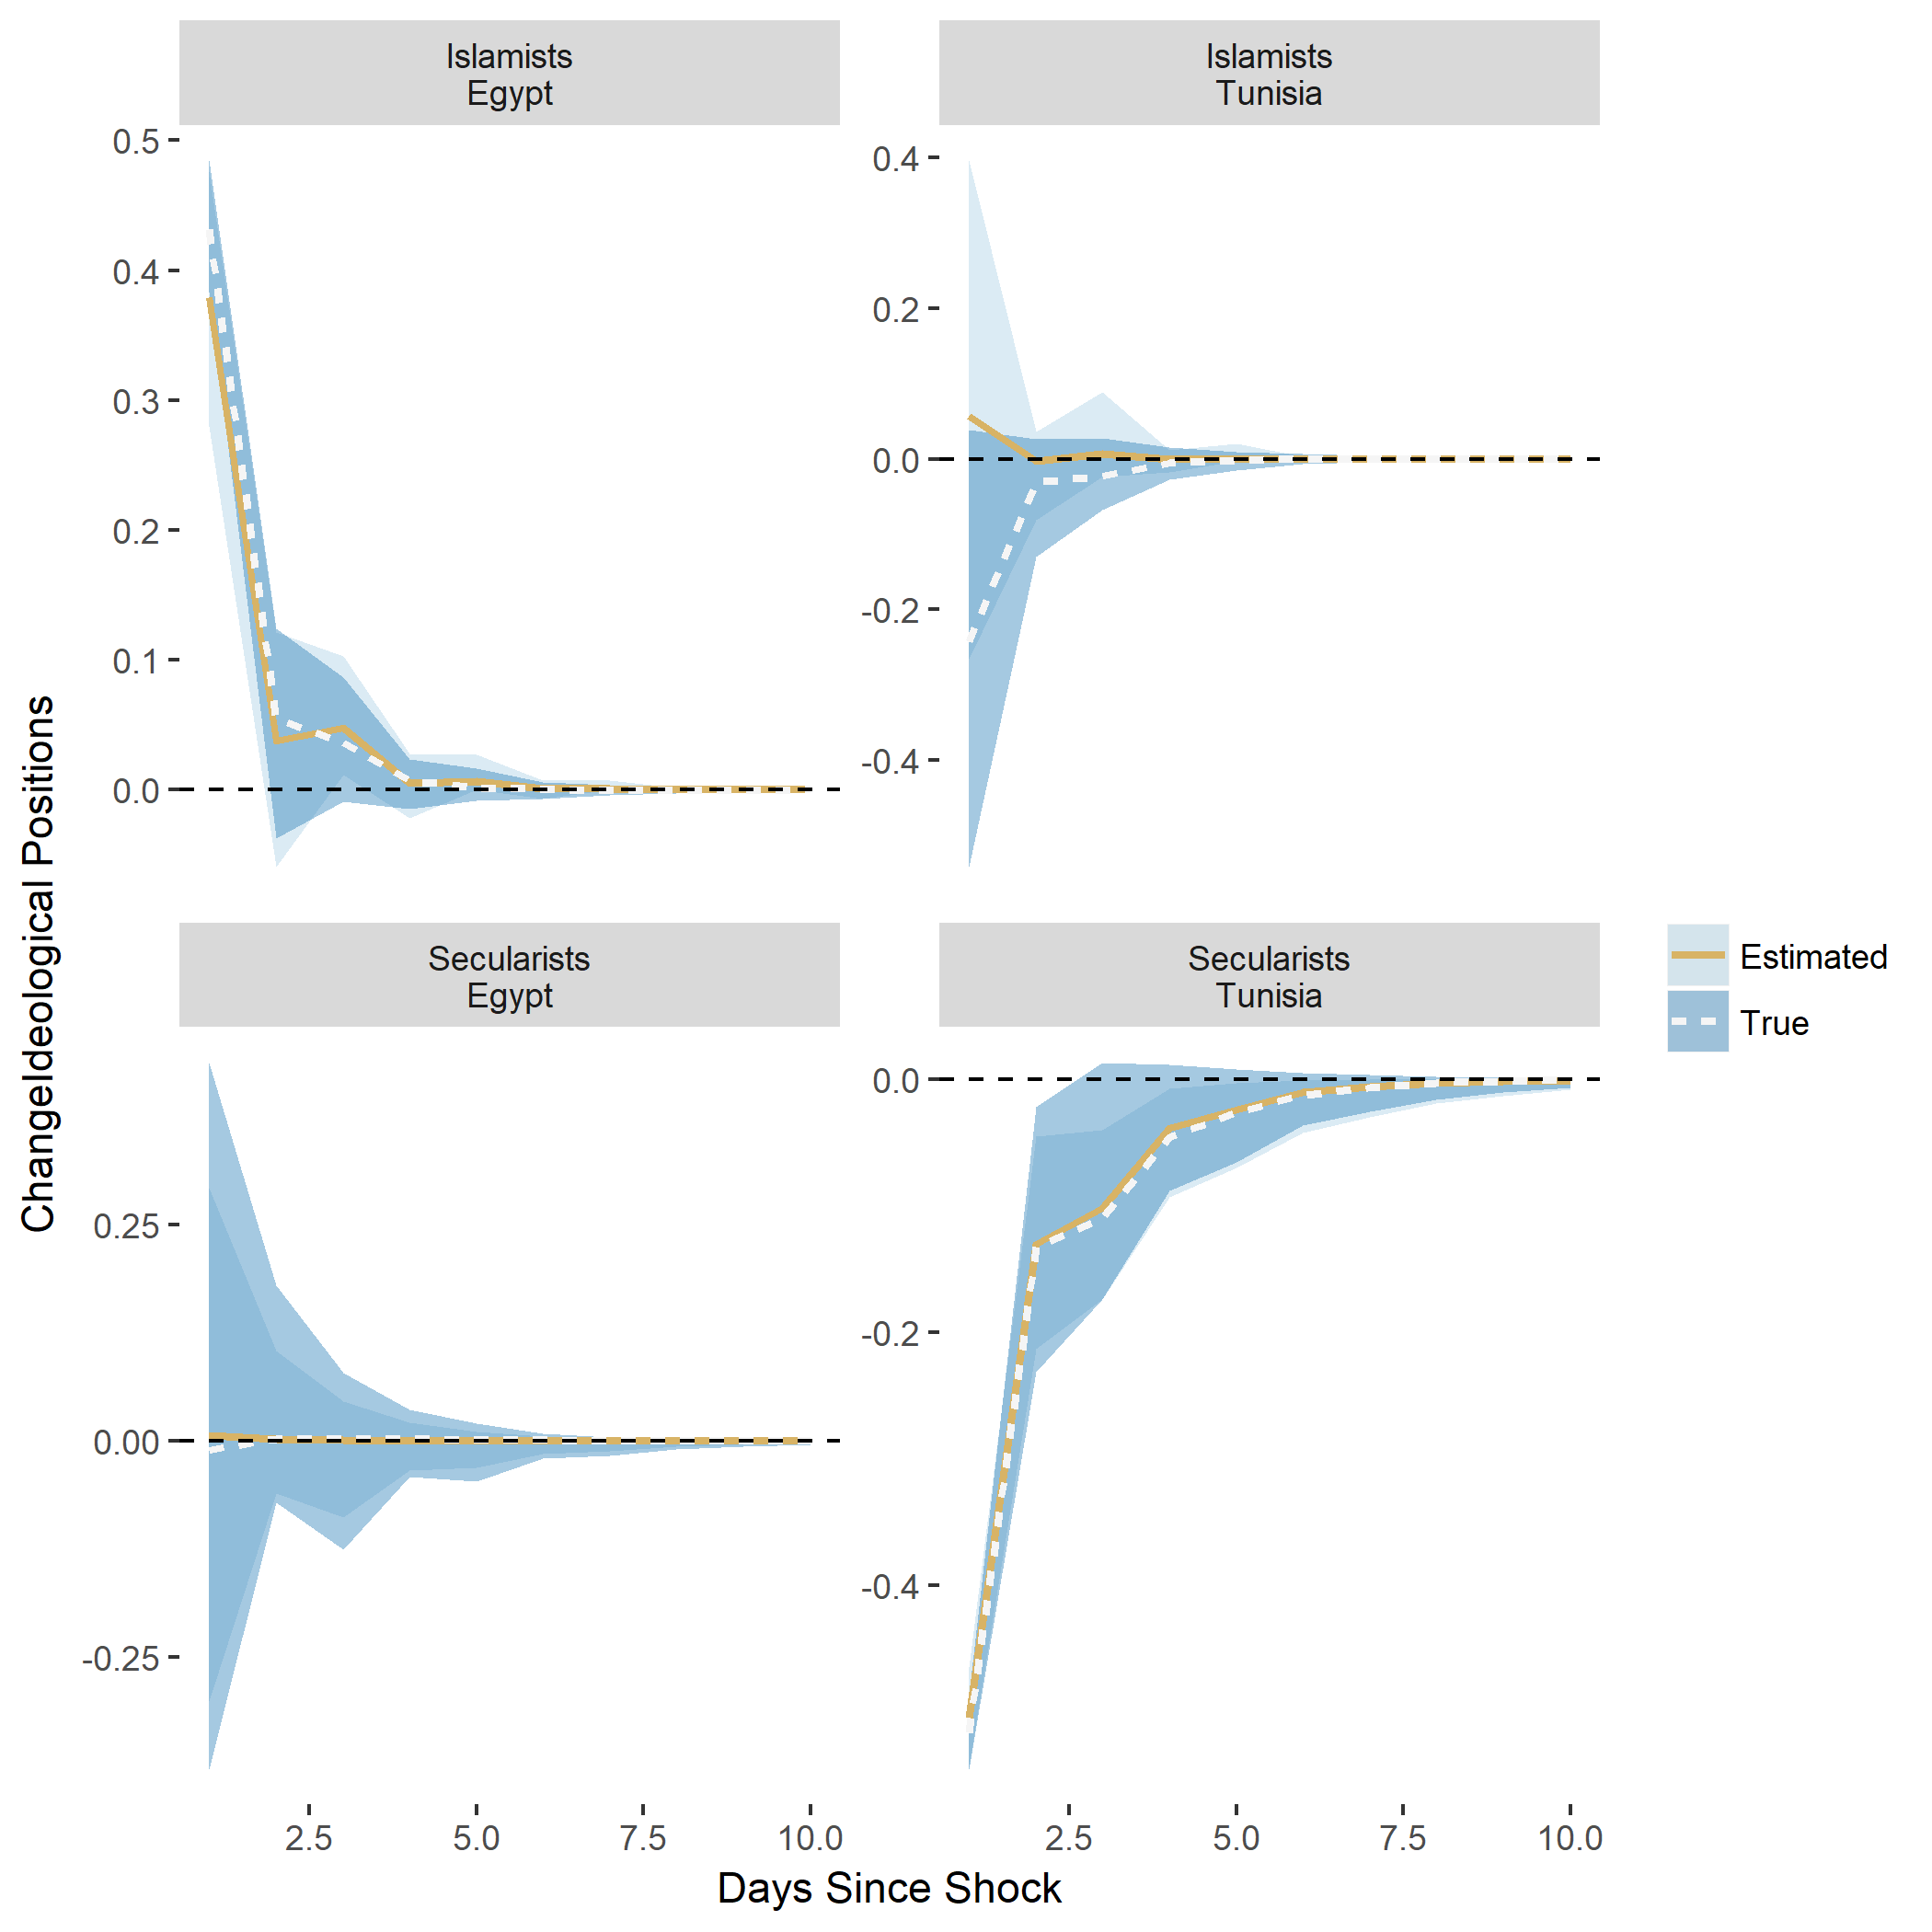
\includegraphics[width=.9\linewidth]{irf_simulation_panels}
\end{figure}

Finally, Figure \ref{irf_simulation_panels} shows the performance of the model at recovering the core estimand of interest, impulse response functions, from the latent time series using Bayesian MCMC estimation within the Stan framework \parencite{carpenter2017}. To do so we generated data from a simulated model and then estimated a VAR on the simulated ideal point time series. We then compared these ``true" IRFs to the estimated IRFs from a Bayesian fit. While the recovery is not perfect, it is able to follow the same path of the generated data. The uncertainty around the latent process will by necessity be larger because the time series themselves are unobserved.

\printbibliography






\end{document}